\documentclass[]{article}
\usepackage{lmodern}
\usepackage{amssymb,amsmath}
\usepackage{ifxetex,ifluatex}
\usepackage{fixltx2e} % provides \textsubscript
\ifnum 0\ifxetex 1\fi\ifluatex 1\fi=0 % if pdftex
  \usepackage[T1]{fontenc}
  \usepackage[utf8]{inputenc}
\else % if luatex or xelatex
  \ifxetex
    \usepackage{mathspec}
  \else
    \usepackage{fontspec}
  \fi
  \defaultfontfeatures{Ligatures=TeX,Scale=MatchLowercase}
\fi
% use upquote if available, for straight quotes in verbatim environments
\IfFileExists{upquote.sty}{\usepackage{upquote}}{}
% use microtype if available
\IfFileExists{microtype.sty}{%
\usepackage{microtype}
\UseMicrotypeSet[protrusion]{basicmath} % disable protrusion for tt fonts
}{}
\usepackage[margin=1in]{geometry}
\usepackage{hyperref}
\hypersetup{unicode=true,
            pdftitle={Exerciții de seminar 2},
            pdfborder={0 0 0},
            breaklinks=true}
\urlstyle{same}  % don't use monospace font for urls
\usepackage{natbib}
\bibliographystyle{plainnat}
\usepackage{graphicx,grffile}
\makeatletter
\def\maxwidth{\ifdim\Gin@nat@width>\linewidth\linewidth\else\Gin@nat@width\fi}
\def\maxheight{\ifdim\Gin@nat@height>\textheight\textheight\else\Gin@nat@height\fi}
\makeatother
% Scale images if necessary, so that they will not overflow the page
% margins by default, and it is still possible to overwrite the defaults
% using explicit options in \includegraphics[width, height, ...]{}
\setkeys{Gin}{width=\maxwidth,height=\maxheight,keepaspectratio}
\IfFileExists{parskip.sty}{%
\usepackage{parskip}
}{% else
\setlength{\parindent}{0pt}
\setlength{\parskip}{6pt plus 2pt minus 1pt}
}
\setlength{\emergencystretch}{3em}  % prevent overfull lines
\providecommand{\tightlist}{%
  \setlength{\itemsep}{0pt}\setlength{\parskip}{0pt}}
\setcounter{secnumdepth}{5}
% Redefines (sub)paragraphs to behave more like sections
\ifx\paragraph\undefined\else
\let\oldparagraph\paragraph
\renewcommand{\paragraph}[1]{\oldparagraph{#1}\mbox{}}
\fi
\ifx\subparagraph\undefined\else
\let\oldsubparagraph\subparagraph
\renewcommand{\subparagraph}[1]{\oldsubparagraph{#1}\mbox{}}
\fi

%%% Use protect on footnotes to avoid problems with footnotes in titles
\let\rmarkdownfootnote\footnote%
\def\footnote{\protect\rmarkdownfootnote}

%%% Change title format to be more compact
\usepackage{titling}

% Create subtitle command for use in maketitle
\newcommand{\subtitle}[1]{
  \posttitle{
    \begin{center}\large#1\end{center}
    }
}

\setlength{\droptitle}{-2em}
  \title{Exerciții de seminar 2}
  \pretitle{\vspace{\droptitle}\centering\huge}
  \posttitle{\par}
\subtitle{Regresie}
  \author{}
  \preauthor{}\postauthor{}
  \date{}
  \predate{}\postdate{}

\usepackage{booktabs}
\usepackage{longtable}
\usepackage{framed,color}
\definecolor{shadecolor}{RGB}{248, 248, 248}
%\definecolor{shadecolor1}{RGB}{216,225,235}
%\definecolor{framecolor}{RGB}{108,123,13}

%\definecolor{shadecolor}{RGB}{226, 255, 241}
\definecolor{shadecolor1}{RGB}{217,225,199}
\definecolor{framecolor}{RGB}{60,179,113}

%%%%%%%%%%%%%%%%%%%%%%
\ifxetex
  \usepackage{letltxmacro}
  \setlength{\XeTeXLinkMargin}{1pt}
  \LetLtxMacro\SavedIncludeGraphics\includegraphics
  \def\includegraphics#1#{% #1 catches optional stuff (star/opt. arg.)
    \IncludeGraphicsAux{#1}%
  }%
  \newcommand*{\IncludeGraphicsAux}[2]{%
    \XeTeXLinkBox{%
      \SavedIncludeGraphics#1{#2}%
    }%
  }%
\fi

\newenvironment{frshaded*}{%
  \def\FrameCommand{\fboxrule=\FrameRule\fboxsep=\FrameSep \fcolorbox{framecolor}{shadecolor1}}%
  \MakeFramed {\advance\hsize-\width \FrameRestore}}%
{\endMakeFramed}

\newenvironment{rmdblock}[1]
  {\begin{frshaded*}
  \begin{itemize}
  \renewcommand{\labelitemi}{
    \raisebox{-.7\height}[0pt][0pt]{
      {\setkeys{Gin}{width=2em,keepaspectratio}\includegraphics{images/icons/#1}}
    }
  }
  \item
  }
  {
  \end{itemize}
  \end{frshaded*}
  }
  
%%%%%%%%%%%%%%%
% definitions.
% -------------------
\usepackage{marginnote}
% \renewcommand*{\marginnotevadjust}{40pt}
% \renewcommand{\marginnotevadjust}{0pt}
% \renewcommand{\marginfont}{\noindent\rule{0pt}{0.7\baselineskip}\tiny}

\newtheorem{proposition}{Proposition}[section]
\newtheorem{lemma}[proposition]{Lemma}
\newtheorem{corollary}[proposition]{Corollary}
\newtheorem{theorem}[proposition]{Theorem}

\newcounter{exo}[section]
\newcommand{\enonce}[2]{\refstepcounter{proposition}\hypertarget{exo:#1}{}\label{exo:#1}{\scriptsize\;\textbf{Ex.}~\ref{exo:#1}}}

\reversemarginpar
\setlength{\marginparwidth}{1.2cm}
% 
% \newcommand{\enonce}[2]{\refstepcounter{proposition}\hypertarget{exo:#1}{}\label{exo:#1}{\noindent\color{black}\normalsize\bf Exercice \ref{exo:#1}}\ \  #2\vspace{1mm}\hrule\vspace{1mm} \color{black}\normalsize}


%%%%%%%%%%%%%%%

\newenvironment{rmdcaution}
  {\begin{rmdblock}{caution}}
  {\end{rmdblock}}
% \newenvironment{rmdinsight}
%   {\begin{rmdblock}{insight}}
%   {\end{rmdblock}}

\newenvironment{rmdexercise}
  {\begin{rmdblock}{exercise}}
  {\end{rmdblock}}

% \newenvironment{rmdexercise_tex}
%   {\begin{rmdblock}{exercise}}
%   {\end{rmdblock}}
  
\newenvironment{rmdtip}
  {\begin{rmdblock}{tip}}
  {\end{rmdblock}}


%%%%%%%%%%%%%%%%%%%%%%%%%%%%%%%%%%%%%%%%%%%%%%%%%%%%%%%%%%%%%%%%%%%%%%%%%%%%%%%%%%%%%%%%%%%%%%%%%%%%%%%%%%%%%%%%%%%%%
%%%%%%%%%%% For insight block %%%%%%%%%%%%%%%%%%%%%%%%%%
\definecolor{shadecolor_insight}{RGB}{223,240,216}
\definecolor{framecolor_insight}{RGB}{136,193,137}

%\definecolor{shadecolor_insight}{RGB}{217,225,199}
%\definecolor{framecolor_insight}{RGB}{60,179,113}

\newenvironment{frshaded_insight*}{%
  \def\FrameCommand{\fboxrule=\FrameRule\fboxsep=\FrameSep \fcolorbox{framecolor_insight}{shadecolor_insight}}%
  \MakeFramed {\advance\hsize-\width \FrameRestore}}%
{\endMakeFramed}

\newenvironment{rmdblock_insight}[1]
  {\begin{frshaded_insight*}
  \begin{itemize}
  \renewcommand{\labelitemi}{
    \raisebox{-.7\height}[0pt][0pt]{
      {\setkeys{Gin}{width=2em,keepaspectratio}\includegraphics{images/icons/#1}}
    }
  }
  \item
  }
  {
  \end{itemize}
  \end{frshaded_insight*}
  }

\newenvironment{rmdinsight}
  {\begin{rmdblock_insight}{insight}}
  {\end{rmdblock_insight}}

%%%%%%%%%%%%%%%%%%%%%%%%%%%%%%%%%%%%%%%%%%%%%%%%%%%%%%%%%%%%%%%%%%%%%%%%%%%%%%%%%%%%%%%%%%%%%%%%%%%%%%%%%%%%%%%%%%%%%
\usepackage{subfigure}
\usepackage{booktabs}
\usepackage{slashbox}
\usepackage{color}
%%%%%%%%%%%%%%%%%%%%%%%%%%%%%%%%%%%%%%%%%
\definecolor{linkcol}{rgb}{0,0,0.4}
\definecolor{citecol}{rgb}{0.5,0,0}

% Change this to change the informations included in the pdf file
% \usepackage[pagebackref]{hyperref}
% \usepackage[verbose]{backref}
\usepackage[hyperpageref]{backref}
% \backrefsetup{verbose=false}
% \PassOptionsToPackage{pagebackref}{hyperref}
% See hyperref documentation for information on those parameters

\hypersetup
{
bookmarksopen=true,
pdftitle="Curs Instrumente Statistice pentru Finante",
pdfauthor="Alexandru Amarioarei",
pdfsubject="Laboratoare Instrumente Statistice pentru Finante", %subject of the document
pdfmenubar=true, %menubar shown
pdfhighlight=/O, %effect of clicking on a link
colorlinks=true, %couleurs sur les liens hypertextes
pdfpagemode=None, %aucun mode de page
pdfpagelayout=SinglePage, %ouverture en simple page
pdffitwindow=true, %pages ouvertes entierement dans toute la fenetre
linkcolor=linkcol, %couleur des liens hypertextes internes
citecolor=citecol, %couleur des liens pour les citations
urlcolor=linkcol %couleur des liens pour les url
}


% set the back references
\renewcommand*{\backref}[1]{}
\renewcommand*{\backreftwosep}{ și~} % inserted between entries 
                              % in a list of two entries, 
                              % default is " and~".
\renewcommand*{\backreflastsep}{ și~} % inserted between the last 
                               % two entries of a list with more
                               % than two entries, default is ", and~".
\renewcommand*{\backrefalt}[4]{%
    \ifcase #1 (Necitat.)%
    \or        (Citat la pagina~#2.)%
    \else      (Citat la paginile~#2.)%
    \fi}

%%%%%%%%%%%%%%%%%%%%%%%%%%%%%%%%%%%%%%%%%%%%%%%%%%%%%%%%%%%%%%%%%%%%%%%%%%%%%%%%%%%%%%%%%%%%%%%%%%%%%%%%%%%%%%%%%%%%%
%CITEVA DEFINITII
\def\om{\omega}
\def\Om{\Omega}
\def\et{\eta}
\def\td{\tilde{\delta}}
\def\m{{\mu}}
\def\n{{\nu}}
\def\k{{\kappa}}
\def\l{{\lambda}}
\def\L{{\Lambda}}
\def\g{{\gamma}}
\def\a{{\alpha}}
\def\e{{\varepsilon}}
\def\b{{\beta}}
\def\G{{\Gamma}}
\def\d{{\delta}}
\def\D{{\Delta}}
\def\t{{\theta}}
\def\s{{\sigma}}
\def\S{{\Sigma}}
\def\z{{\zeta}}
\def\qed{\hfill\Box}
\def\ds{\displaystyle}
\def\mc{\mathcal}
%%%%%%%%%%%%%%%%%%%%%%%%%%%%%%%%%%%%%%%%%%%%%%%%%%%%%%%%%%%%%%%%%%%%%%%%%%%%%%%%%%%%%%%%%%%%%%%%%%%%%%%%%%%%%%%%%%%%%%
\def\1{{\mathbf 1}}
\def\CC{{\mathbb C}}
\def\VV{{\mathbb V}}
\def\RR{{\mathbb R}}
\def\QQ{{\mathbb Q}}
\def\ZZ{{\mathbb Z}}
\def\PP{{\mathbb P}}
\def\EE{{\mathbb E}}
\def\NN{{\mathbb N}}
\def\FF{{\mathbb F}}
%\def\SS{{\mathbb S}}
\def\MA{{\mathcal A}}
\def\MO{{\mathcal O}}
\def\MF{{\mathcal F}}
\def\ME{{\mathcal E}}
\def\MR{{\mathcal R}}
\def\MB{{\mathcal B}}
\def\MM{{\mathcal M}}
\def\MN{{\mathcal N}}
\def\MU{{\mathcal U}}
\def\MP{{\mathcal P}}
\def\MS{{\mathcal S}}
\def\MBS{{\mathbf S}}
\def\MX{{\bm{ \mathscr X}}}

% independent sign
\newcommand\independent{\protect\mathpalette{\protect\independenT}{\perp}}
\def\independenT#1#2{\mathrel{\rlap{$#1#2$}\mkern2mu{#1#2}}}

\renewcommand\tablename{Tab.}
\renewcommand{\figurename}{Fig.}
\renewcommand\refname{Referințe}

%%%%%%%%%%%%%%%%%%%%%%%%%%%%%%%%%%%%%%%%%%%%%%%%%%%%%%%%%%%%%%%%%%%%%%%%%%%%%%%%%%%%%%%%%%%%%%%%%%%%%%%%%%%%%%%%%%%%%
%Header and Footer
\usepackage{fancyhdr}

\pagestyle{fancy}
\fancyhf{}
\rhead{Universitatea din Bucure\c sti\\ Facultatea de Matematic\u a \c si Informatic\u a}
\lhead{\textit{Curs}: Instrumente Statistice pentru Finan\c te\\ \textit{Instructor}: A. Am\u arioarei}
\rfoot{Pagina \thepage}
\lfoot{Grupa: 403}
%%%%%%%%%%%%%%%%%%%%%%%%%%%%%%%%%%%%%%%
\usepackage{booktabs}
\usepackage{longtable}
\usepackage{array}
\usepackage{multirow}
\usepackage[table]{xcolor}
\usepackage{wrapfig}
\usepackage{float}
\usepackage{colortbl}
\usepackage{pdflscape}
\usepackage{tabu}
\usepackage{threeparttable}
\usepackage{threeparttablex}
\usepackage[normalem]{ulem}
\usepackage{makecell}

\begin{document}
\maketitle

%%%%%%%%%%%%%%%%%%%%%%%%
\thispagestyle{fancy}

Obiectivul acestui seminar este de a prezenta câteva exerciții de
regresie liniară.

\section{Regresie liniară simplă}\label{regresie-liniara-simpla}

\subsection{Metoada celor mai mici
pătrate}\label{metoada-celor-mai-mici-patrate}

\begin{rmdexercise}
\marginnote{\enonce{12001}{}}\vspace{-7mm}

Arătați că estimatorii \(\hat{\beta}_0\) și \(\hat{\beta}_1\) obținuți
prin metoda celor mai mici pătrate, adică valorile coeficienților
\(\beta_0\) și \(\beta_1\) care minimizează funcția

\[
  S(\beta_0, \beta_1) = \sum_{i = 1}^{n}(y_i - \beta_0 - \beta_1 x_i)^2
\]

sunt dați de expresiile

\[
  \hat\beta_0 = \bar y - \hat\beta_1 \bar x \quad \text{și} \quad \hat\beta_1 = \frac{\sum_{i = 1}^{n}(x_i - \bar x)(y_i - \bar y)}{\sum_{i = 1}^{n}(x_i - \bar x)^2}.
\]
\end{rmdexercise}

Trebuie să determinăm

\[
  (\hat{\beta}_0, \hat{\beta}_1) = \underset{(\beta_0,\beta_1)\in\mathbb{R}\times\mathbb{R}}{\arg\min} S(\beta_0, \beta_1)
\]

și observând că funcția \(S(\beta_0, \beta_1)\) este convexă ea admite
un punct de minim. Acesta se obține ca soluție a sistemului
\(\nabla S = 0\) de ecuați normale,

\[
\left\{\begin{array}{ll}
  \frac{\partial S}{\partial \beta_0} = -2\sum_{i = 1}^{n}(y_i - \beta_0 - \beta_1 x_i) = 0\\
  \frac{\partial S}{\partial \beta_1} = -2\sum_{i = 1}^{n}x_i(y_i - \beta_0 - \beta_1 x_i) = 0
\end{array}\right.
\]

Din prima ecuație obținem prin sumare
\(n\beta_0 + \beta_1\sum_{i=1}^{n}x_i = \sum_{i=1}^{n}y_i\) ceea ce
conduce la \(\hat\beta_0 = \bar y - \hat\beta_1 \bar x\).

A doua ecuație conduce la

\[
  \beta_0\sum_{i=1}^{n}x_i + \beta_1\sum_{i=1}^{n}x_i^2 = \sum_{i=1}^{n}x_iy_i
\]

și înlocuind \(\beta_0\) cu expresia obținută anterior, obținem soluția

\[
\hat\beta_1 = \frac{\sum_{i = 1}^{n}x_i(y_i - \bar y)}{\sum_{i = 1}^{n}x_i(x_i - \bar x)} = \frac{\sum_{i = 1}^{n}(x_i - \bar x)(y_i - \bar y)}{\sum_{i = 1}^{n}(x_i - \bar x)^2}.
\]

De asemenea, se poate verifica că \(S(\beta_0, \beta_1)\) se scrie sub
forma

\begin{align*}
  S(\beta_0, \beta_1) &= n\left[\beta_0 - (\bar y - \beta_1\bar x)\right]^2 + \left[\sum_{i = 1}^{n}(x_i - \bar x)^2\right]\left[\beta_1 - \frac{\sum_{i = 1}^{n}(x_i - \bar x)(y_i - \bar y)}{\sum_{i = 1}^{n}(x_i - \bar x)^2}\right]^2 \\
  &\quad + \left[\sum_{i = 1}^{n}(y_i - \bar y)^2\right]\left[1 - \frac{\left(\sum_{i = 1}^{n}(x_i - \bar x)(y_i - \bar y)\right)^2}{\sum_{i = 1}^{n}(x_i - \bar x)^2\sum_{i = 1}^{n}(y_i - \bar y)^2}\right]
\end{align*}

care justifică în egală măsură soluția obținută anterior.

\begin{rmdexercise}
\marginnote{\enonce{12002}{}}\vspace{-7mm}

Arătați că estimatorii obținuți prin metoda celor mai mici pătrate,
\(\hat\beta_0\) și \(\hat\beta_1\), sunt estimatori nedeplasați.
\end{rmdexercise}

Coeficienții \(\hat\beta_0\) și \(\hat\beta_1\) obținuți prin metoda
celor mai mici pătrate sunt dați de
\(\hat\beta_0 = \bar y - \hat\beta_1 \bar x\) și
\(\hat\beta_1 = \frac{\sum_{i = 1}^{n}(x_i - \bar x)(y_i - \bar y)}{\sum_{i = 1}^{n}(x_i - \bar x)^2}\)
(aceștia sunt variabile aleatoare deoarece sunt funcții de \(Y_i\) care
sunt variabile aleatoare). Înlocuind în expresia lui \(\hat\beta_1\) pe
\(y_i\) cu \(\beta_0+\beta_1 x_i + \varepsilon_i\) avem

\begin{align*}
\hat\beta_1 &= \frac{\sum_{i = 1}^{n}(x_i - \bar x)(y_i - \bar y)}{\sum_{i = 1}^{n}(x_i - \bar x)^2} = \frac{\sum_{i = 1}^{n}(x_i - \bar x)y_i}{\sum_{i = 1}^{n}(x_i - \bar x)^2} = \frac{\sum_{i = 1}^{n}(x_i - \bar x)(\beta_0+\beta_1 x_i + \varepsilon_i)}{\sum_{i = 1}^{n}(x_i - \bar x)^2}\\
  &= \frac{\beta_0\overbrace{\sum_{i = 1}^{n}(x_i - \bar x)}^{ = 0} + \beta_1 \sum_{i = 1}^{n}(x_i - \bar x)x_i + \sum_{i = 1}^{n}(x_i - \bar x)\varepsilon_i}{\sum_{i = 1}^{n}(x_i - \bar x)^2} = \frac{\beta_1 \sum_{i = 1}^{n}(x_i - \bar x)^2 + \sum_{i = 1}^{n}(x_i - \bar x)\varepsilon_i}{\sum_{i = 1}^{n}(x_i - \bar x)^2}\\
  &= \beta_1 + \frac{\sum_{i = 1}^{n}(x_i - \bar x)\varepsilon_i}{\sum_{i = 1}^{n}(x_i - \bar x)^2}.
\end{align*}

Conform ipotezei modelului de regresie liniară simplă,
\(\mathbb{E}[\varepsilon_i] = 0\), prin urmare
\(\mathbb{E}[\hat\beta_1] = \beta_1\) ceea ce arată că \(\hat\beta_1\)
este un estimator nedeplasat pentru \(\beta_1\).

În mod similar,

\[
\mathbb{E}[\hat\beta_0] = \mathbb{E}[\bar y] - \bar x\mathbb{E}[\hat\beta_1] = \beta_0 + \bar x\beta_1 - \bar x\beta_1 = \beta_0
\] ceea ce arată că \(\hat\beta_0\) este un estimator nedeplasat pentru
\(\beta_0\).

\begin{rmdexercise}
\marginnote{\enonce{12003}{}}\vspace{-7mm}

Calculați matricea de varianță-covarianță a estimatorilor
\(\hat\beta_0\) și \(\hat\beta_1\).
\end{rmdexercise}

Notăm cu
\(W = \begin{pmatrix}Var(\hat \beta_0) & Cov(\hat \beta_0, \hat \beta_1)\\ Cov(\hat \beta_0, \hat \beta_1) & Var(\hat \beta_1)\end{pmatrix}\)
matricea de varianță-covarianță a estimatorilor \(\hat\beta_0\) și
\(\hat\beta_1\).

Avem, folosind expresia lui \(\hat\beta_1\) determinată la punctul
anterior și homoscedasticitatea și necorelarea erorilor
\(Cov(\varepsilon_i, \varepsilon_j) = \delta_{ij}\sigma^2\), că

\begin{align*}
  Var(\hat \beta_1) &= Var\left(\beta_1 + \frac{\sum_{i = 1}^{n}(x_i - \bar x)\varepsilon_i}{\sum_{i = 1}^{n}(x_i - \bar x)^2}\right) = Var\left(\frac{\sum_{i = 1}^{n}(x_i - \bar x)\varepsilon_i}{\sum_{i = 1}^{n}(x_i - \bar x)^2}\right)\\
  &= \frac{Var\left(\sum_{i = 1}^{n}(x_i - \bar x)\varepsilon_i\right)}{\left[\sum_{i = 1}^{n}(x_i - \bar x)^2\right]^2} = \frac{\sum_{i,j}(x_i - \bar x)(x_j - \bar x)Cov(\varepsilon_i, \varepsilon_j)}{\left[\sum_{i = 1}^{n}(x_i - \bar x)^2\right]^2}\\
  &= \frac{\sum_{i = 1}^{n}(x_i - \bar x)^2\sigma^2}{\left[\sum_{i = 1}^{n}(x_i - \bar x)^2\right]^2} = \frac{\sigma^2}{\sum_{i = 1}^{n}(x_i - \bar x)^2}.
\end{align*}

Din expresia \(Var(\hat \beta_1)\) observăm că dacă \(\sigma^2\) este
mică (cu alte cuvinte \(y_i\) sunt aproape de dreapta de regresie)
atunci estimarea este mai precisă. De asemenea, se constată că pe măsură
ce valorile \(x_i\) sunt mai dispersate în jurul valorii medii
\(\bar x\) estimarea coeficientului \(\hat \beta_1\) este mai precisă
(\(Var(\hat \beta_1)\) este mai mică). Acest fenomen se poate observa și
în figura de mai jos în care am generat \(100\) de valori aleatoare
\(X\) și \(100\) de valori pentru \(Y\) după modelul

\[
  y = 1 + 2 x + \varepsilon
\] cu \(\varepsilon\sim \mathcal{N}(0, \sigma^2)\). Dreapta roșie
descrie adevărata relație \(f(x) = 1 + 2x\) în populație iar dreapta
albastră reprezintă dreapta de regresie calculată cu ajutorul metodei
celor mai mici pătrate (OLS). Dreptele albastru deschis au fost generate
tot cu ajutorul metodei celor mai mici pătrate atunci când variem
\(\sigma^2\) (în figura din stânga) și respectiv pe \(x_i\) în jurul lui
\(\bar x\) (în figura din dreapta).

\begin{center}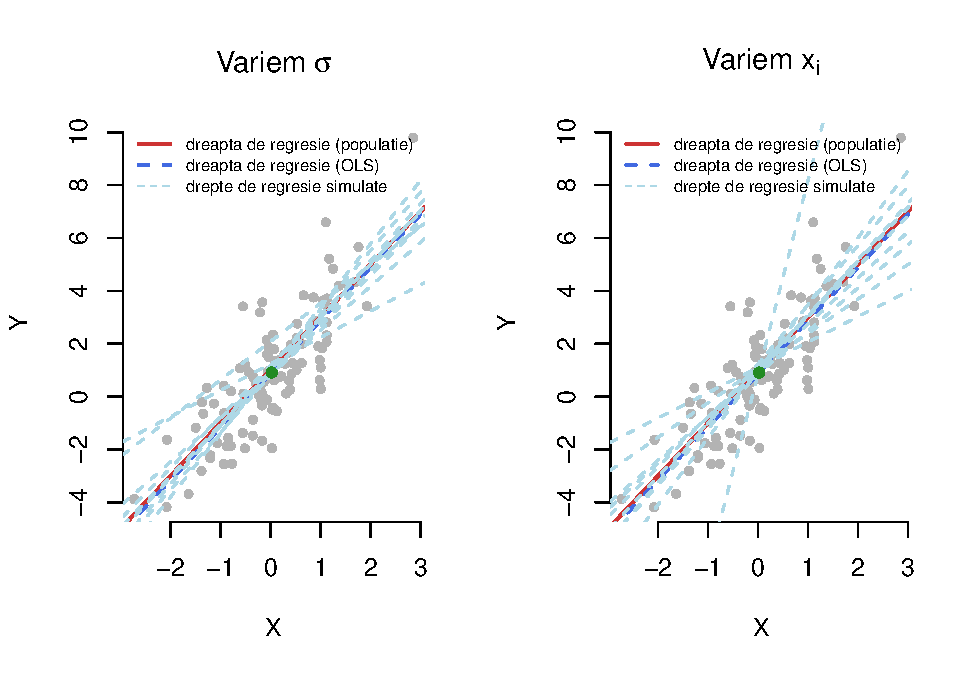
\includegraphics[width=0.8\linewidth]{Sem_2_files/figure-latex/unnamed-chunk-5-1} \end{center}

Pentru a determina \(Var(\hat \beta_0)\), vom folosi relația
\(\hat \beta_0 = \bar y - \hat \beta_1 \bar x\) ceea ce conduce la

\begin{align*}
Var(\hat \beta_0) &= Var(\bar y - \hat \beta_1 \bar x) = Var(\bar y) - 2Cov(\bar y, \hat \beta_1 \bar x) + Var(\hat \beta_1 \bar x)\\
&= Var\left(\frac{1}{n}\sum_{i = 1}^{n}y_i\right) - 2\bar x Cov(\bar y, \hat \beta_1) + \bar x^2 Var(\hat \beta_1)\\
&= \frac{\sigma^2}{n} + \bar x^2 \frac{\sigma^2}{\sum_{i = 1}^{n}(x_i - \bar x)^2} - 2\bar x Cov(\bar y, \hat \beta_1).
\end{align*}

Pentru \(Cov(\bar y, \hat \beta_1)\) avem (ținând cont de faptul că
\(\beta_0\), \(\beta_1\) și \(x_i\) sunt constante)

\begin{align*}
Cov(\bar y, \hat \beta_1) &= Cov\left(\frac{1}{n}\sum_{i = 1}^{n}y_i, \beta_1 + \frac{\sum_{j = 1}^{n}(x_j - \bar x)\varepsilon_j}{\sum_{j = 1}^{n}(x_j - \bar x)^2} \right) = \frac{1}{n}\sum_{i = 1}^{n}Cov\left(\beta_0 + \beta_1 x_i + \varepsilon_i, \beta_1 + \frac{\sum_{j = 1}^{n}(x_j - \bar x)\varepsilon_j}{\sum_{j = 1}^{n}(x_j - \bar x)^2}\right)\\
&= \frac{1}{n}\sum_{i = 1}^{n}Cov\left(\varepsilon_i, \frac{\sum_{j = 1}^{n}(x_j - \bar x)\varepsilon_j}{\sum_{j = 1}^{n}(x_j - \bar x)^2}\right) = \frac{1}{n}\sum_{i = 1}^{n}\frac{1}{\sum_{j = 1}^{n}(x_j - \bar x)^2}Cov\left(\varepsilon_i, \sum_{j = 1}^{n}(x_j - \bar x)\varepsilon_j\right)\\
&= \frac{1}{\sum_{j = 1}^{n}(x_j - \bar x)^2}\sum_{i = 1}^{n}\frac{1}{n}\sum_{j = 1}^{n}(x_j - \bar x)Cov(\varepsilon_i, \varepsilon_i=j) = \frac{1}{\sum_{j = 1}^{n}(x_j - \bar x)^2}\sum_{i = 1}^{n}\frac{1}{n}\sum_{j = 1}^{n}(x_j - \bar x)\delta_{ij}\sigma^2\\
&= \frac{\sigma^2}{\sum_{j = 1}^{n}(x_j - \bar x)^2}\frac{1}{n}\underbrace{\sum_{i = 1}^{n}(x_i - \bar x)}_{=0} = 0
\end{align*}

prin urmare

\[
Var(\hat \beta_0) = \frac{\sigma^2}{n} + \bar x^2 \frac{\sigma^2}{\sum_{i = 1}^{n}(x_i - \bar x)^2} = \frac{\sigma^2\sum_{i = 1}^{n}x_i^2}{n\sum_{i = 1}^{n}(x_i - \bar x)^2}.
\]

Calculul covarianței dintre \(\hat \beta_0\) și \(\hat \beta_1\) rezultă
aplicând relațiile de mai sus

\[
Cov(\hat \beta_0, \hat \beta_1) = Cov(\bar y - \hat \beta_1\bar x, \hat \beta_1) = Cov(\bar y, \hat \beta_1) - \bar x Var(\hat \beta_1) = -\frac{\sigma^2 \bar x}{\sum_{i = 1}^{n}(x_i - \bar x)^2}.
\]

Observăm că \(Cov(\hat \beta_0, \hat \beta_1)\leq 0\) iar intuitiv, cum
dreapta de regresie (bazată pe estimatorii obținuți prin metoda celor
mai mici pătrate) \(\bar y = \hat\beta_0 + \hat\beta_1 \bar x\) trece
prin centrul de greutate al datelor \((\bar x, \bar y)\), dacă
presupunem \(\bar x > 0\) remarcăm că atunci când creștem panta (creștem
\(\hat\beta_1\)) ordonata la origine scade (scade \(\hat\beta_0\)) și
reciproc.

Matricea de varianță-covarianță a estimatorilor \(\hat\beta_0\) și
\(\hat\beta_1\) devine

\[
W = \begin{pmatrix}Var(\hat \beta_0) & Cov(\hat \beta_0, \hat \beta_1)\\ Cov(\hat \beta_0, \hat \beta_1) & Var(\hat \beta_1)\end{pmatrix} = \begin{pmatrix}\frac{\sigma^2\sum_{i = 1}^{n}x_i^2}{n\sum_{i = 1}^{n}(x_i - \bar x)^2} & -\frac{\sigma^2 \bar x}{\sum_{i = 1}^{n}(x_i - \bar x)^2}\\ -\frac{\sigma^2 \bar x}{\sum_{i = 1}^{n}(x_i - \bar x)^2} & \frac{\sigma^2}{\sum_{i = 1}^{n}(x_i - \bar x)^2}\end{pmatrix}.
\]

\begin{rmdexercise}
\marginnote{\enonce{12004}{}}\vspace{-7mm}

Arătați că în cadrul modelului de regresie liniară simplă, suma
valorilor reziduale este nulă.
\end{rmdexercise}

Observăm, folosind definiția \(\hat\varepsilon_i = y_i - \hat y_i\), că

\begin{align*}
  \sum_{i = 1}^{n}\hat\varepsilon_i &= \sum_{i = 1}^{n}(y_i - \hat y_i) = \sum_{i = 1}^{n}(y_i - \hat \beta_0 - x_i\hat\beta_1)\\
    &= \sum_{i = 1}^{n}\left[y_i - \underbrace{(\bar y - \bar x\hat\beta_1)}_{= \hat \beta_0} - x_i\hat\beta_1\right] = \sum_{i = 1}^{n}(y_i - \bar y) -\hat\beta_1 \sum_{i = 1}^{n}(x_i - \bar x) = 0
\end{align*}

\begin{rmdexercise}
\marginnote{\enonce{12005}{}}\vspace{-7mm}

Arătați că în modelul de regresie liniară simplă statistica
\(\hat\sigma^2 = \frac{1}{n-2}\sum_{i = 1}^{n}\hat\varepsilon_i^2\) este
un estimator nedeplasat pentru \(\sigma^2\).
\end{rmdexercise}

Ținând cont de faptul că \(\hat\beta_0 = \bar y - \hat\beta_1 \bar x\)
și \(\bar y = \beta_0 + \beta_1 \bar x + \bar \varepsilon\) (prin
însumarea după \(i\) a relațiilor
\(y_i = \beta_0 + \beta_1 x_i +\varepsilon_i\)) găsim că

\begin{align*}
\hat\varepsilon_i &= y_i - \hat y_i = (\beta_0 + \beta_1 x_i +\varepsilon_i) - (\hat\beta_0 + \hat\beta_1 x_i) \\
  &= (\underbrace{\bar y - \beta_1 \bar x - \bar \varepsilon}_{=\beta_0} + \beta_1 x_i +\varepsilon_i) - (\bar y - \hat\beta_1 \bar x + \hat\beta_1 x_i)\\
  &= (\beta_1 - \hat\beta_1)(x_i - \bar x) + (\varepsilon_i - \bar\varepsilon)
\end{align*}

și prin dezvoltarea binomului și utilizând relația
\(\hat\beta_1 = \beta_1 + \frac{\sum_{i = 1}^{n}(x_i - \bar x)\varepsilon_i}{\sum_{i = 1}^{n}(x_i - \bar x)^2}\)
găsim

\begin{align*}
  \sum_{i = 1}^{n}\hat\varepsilon_i^2 &= (\beta_1 - \hat\beta_1)^2\sum_{i = 1}^{n}(x_i - \bar x) + \sum_{i = 1}^{n}(\varepsilon_i - \bar\varepsilon)^2 + 2(\beta_1 - \hat\beta_1)\sum_{i = 1}^{n}(x_i - \bar x)(\varepsilon_i - \bar\varepsilon)\\
    &= (\beta_1 - \hat\beta_1)^2\sum_{i = 1}^{n}(x_i - \bar x) + \sum_{i = 1}^{n}(\varepsilon_i - \bar\varepsilon)^2 + 2(\beta_1 - \hat\beta_1)\sum_{i = 1}^{n}(x_i - \bar x)\varepsilon_i - 2(\beta_1 - \hat\beta_1)\bar\varepsilon\sum_{i = 1}^{n}(x_i - \bar x)\\
    &= (\beta_1 - \hat\beta_1)^2\sum_{i = 1}^{n}(x_i - \bar x) + \sum_{i = 1}^{n}(\varepsilon_i - \bar\varepsilon)^2 - 2(\beta_1 - \hat\beta_1)^2\sum_{i = 1}^{n}(x_i - \bar x)^2\\
    &=\sum_{i = 1}^{n}(\varepsilon_i - \bar\varepsilon)^2 - (\beta_1 - \hat\beta_1)^2\sum_{i = 1}^{n}(x_i - \bar x)^2.
\end{align*}

Luând media găsim că

\[
\mathbb{E}\left(\sum_{i = 1}^{n}\hat\varepsilon_i^2\right) = \mathbb{E}\left(\sum_{i = 1}^{n}(\varepsilon_i - \bar\varepsilon)^2\right) - \sum_{i = 1}^{n}(x_i - \bar x)^2 Var(\hat\beta_1) = (n-1)\sigma^2 - \sigma^2 = (n-1)\sigma^2
\]

unde am folosit că
\(\mathbb{E}\left(\frac{1}{n-1}\sum_{i = 1}^{n}(\varepsilon_i - \bar\varepsilon)^2\right) = \sigma^2\)
(deoarece \(Var(\varepsilon_i) = \sigma^2\)).

Concluzionăm că
\(\hat\sigma^2 = \frac{1}{n-2}\sum_{i = 1}^{n}\hat\varepsilon_i^2\) este
un estimator nedeplasat pentru \(\sigma^2\).

\begin{rmdexercise}
\marginnote{\enonce{12006}{}}\vspace{-7mm}

Fie \(x_{n+1}\) o nouă valoare pentru variabila \(X\) și ne propunem să
prezicem valoarea \(y_{n+1}\) conform modelului

\[
  y_{n+1} = \beta_0 + \beta_1 x_{n+1} + \varepsilon_{n+1}
\]

cu \(\mathbb{E}[\varepsilon_{n+1}] = 0\),
\(Var(\varepsilon_{n+1}) = \sigma^2\) și
\(Cov(\varepsilon_{n+1}, \varepsilon_i)=0\) pentru \(i = 1,\ldots,n\).

Arătați că varianța răspunsului mediu prezis este

\[
  Var(\hat y_{n+1}) = \sigma^2\left[\frac{1}{n} + \frac{(x_{n+1} - \bar x)^2}{\sum_{i=1}^{n}(x_i - \bar x)^2}\right]
\]

iar varianța erorii de predicție \(\hat\varepsilon_{n+1}\) satisface
\(\mathbb{E}[\hat\varepsilon_{n+1}] = 0\) și

\[
  Var(\hat\varepsilon_{n+1}) = \sigma^2\left[1 + \frac{1}{n} + \frac{(x_{n+1} - \bar x)^2}{\sum_{i=1}^{n}(x_i - \bar x)^2}\right].
\]
\end{rmdexercise}

Cum \(\hat y_{n+1} = \hat\beta_0 + \hat\beta_1 x_{n+1}\) avem

\begin{align*}
  Var(\hat y_{n+1}) &= Var(\hat\beta_0 + \hat\beta_1 x_{n+1}) = Var(\hat\beta_0) + 2Cov(\hat\beta_0, \hat\beta_1) + x_{n+1}^2Var(\hat\beta_1)\\
  &= \frac{\sigma^2\sum_{i = 1}^{n}x_i^2}{n\sum_{i = 1}^{n}(x_i - \bar x)^2} - 2\frac{\sigma^2 \bar x}{\sum_{i = 1}^{n}(x_i - \bar x)^2} + \frac{\sigma^2x_{n+1}^2}{\sum_{i = 1}^{n}(x_i - \bar x)^2}\\
  &= \frac{\sigma^2}{\sum_{i = 1}^{n}(x_i - \bar x)^2}\left[\frac{1}{n}\sum_{i = 1}^{n}x_i^2 - 2x_{n+1}\bar x + x_{n+1}^2\right]\\
  &= \frac{\sigma^2}{\sum_{i = 1}^{n}(x_i - \bar x)^2}\left[\frac{1}{n}\sum_{i = 1}^{n}(x_i -\bar x)^2 + \bar x^2 - 2x_{n+1}\bar x + x_{n+1}^2\right]\\
  &= \sigma^2\left[\frac{1}{n} + \frac{(x_{n+1} - \bar x)^2}{\sum_{i=1}^{n}(x_i - \bar x)^2}\right].
\end{align*}

Constatăm că atunci când \(x_{n+1}\) este departe de valoarea medie
\(\bar x\) răspunsul mediu are o variabilitate mai mare.

Pentru a obține varianța erorii de predicție
\(\hat\varepsilon_{n+1} = y_{n+1} - \hat y_{n+1}\) să observăm că
\(y_{n+1}\) depinde doar de \(\varepsilon_{n+1}\) pe când
\(\hat y_{n+1}\) depinde de \(\varepsilon_i\), \(i\in\{1,2,\ldots,n\}\).
Din necorelarea erorilor deducem că

\[
  Var(\hat\varepsilon_{n+1}) = Var(y_{n+1} - \hat y_{n+1}) = Var(y_{n+1}) + Var(\hat y_{n+1}) = \sigma^2\left[1 + \frac{1}{n} + \frac{(x_{n+1} - \bar x)^2}{\sum_{i=1}^{n}(x_i - \bar x)^2}\right].
\]

\hypertarget{reg_sim_ex_2}{\subsection{\texorpdfstring{Coeficientul de
determinare \(R^2\) și coeficientul de
corelație}{Coeficientul de determinare R\^{}2 și coeficientul de corelație}}\label{reg_sim_ex_2}}

În această secțiune încercăm să abordăm problema de regresie liniară
simplă într-un context geometric. Din punct de vedere vectorial dispunem
de doi vectori: vectorul \(X = (x_1, x_2, \ldots, x_n)^\intercal\) a
celor \(n\) observații ale variabilei explicative și vectorul
\(Y = (y_1, y_2, \ldots, y_n)^\intercal\) compus din cele \(n\)
observații ale variabilei răspuns, pe care vrem să o explicăm. Cei doi
vectori aparțin spațiului \(\mathbb{R}^n\).

Fie \(\mathbf{1} = (1,1,\ldots,1)^\intercal\in\mathbb{R}^n\) și
\(\mathcal{M}(X)\) subspațiul liniar din \(\mathbb{R}^n\) de dimensiune
\(2\) generat de vectorii \(\{\mathbf{1}, X\}\) (acești vectori nu sunt
coliniari deoarece \(X\) conține cel puțin două elemente distincte).
Notăm cu \(\hat Y\) proiecția ortogonală a lui \(Y\) pe subspațiul
\(\mathcal{M}(X)\) și cum \(\{\mathbf{1}, X\}\) formează o bază în
\(\mathcal{M}(X)\) deducem că există
\(\hat\beta_0, \hat\beta_1\in \mathbb{R}\) astfel ca
\(\hat Y = \hat\beta_0\mathbf{1} + \hat\beta_1 X\). Cum, din definiția
priecției ortogonale, \(\hat Y\) este unicul vector din
\(\mathcal{M}(X)\) care minimizează distanța euclidiană (deci și
pătratul ei)

\[
\left\lVert Y - \hat Y \right\rVert = \sum_{i = 1}^{n}[y_i - (\hat\beta_0 + \hat \beta_1 x_i)]^2
\]

deducem că \(\hat\beta_0, \hat\beta_1\) coincid cu valorile obținute
prin metoda celor mai mici pătrate. Astfel coeficienții \(\hat\beta_0\)
și \(\hat\beta_1\) se reprezintă coordonatele proiecției ortogonale a
lui \(Y\) pe subspațiul generat de vectorii \(\{\mathbf{1}, X\}\) (a se
vedea figura de mai jos).

\begin{center}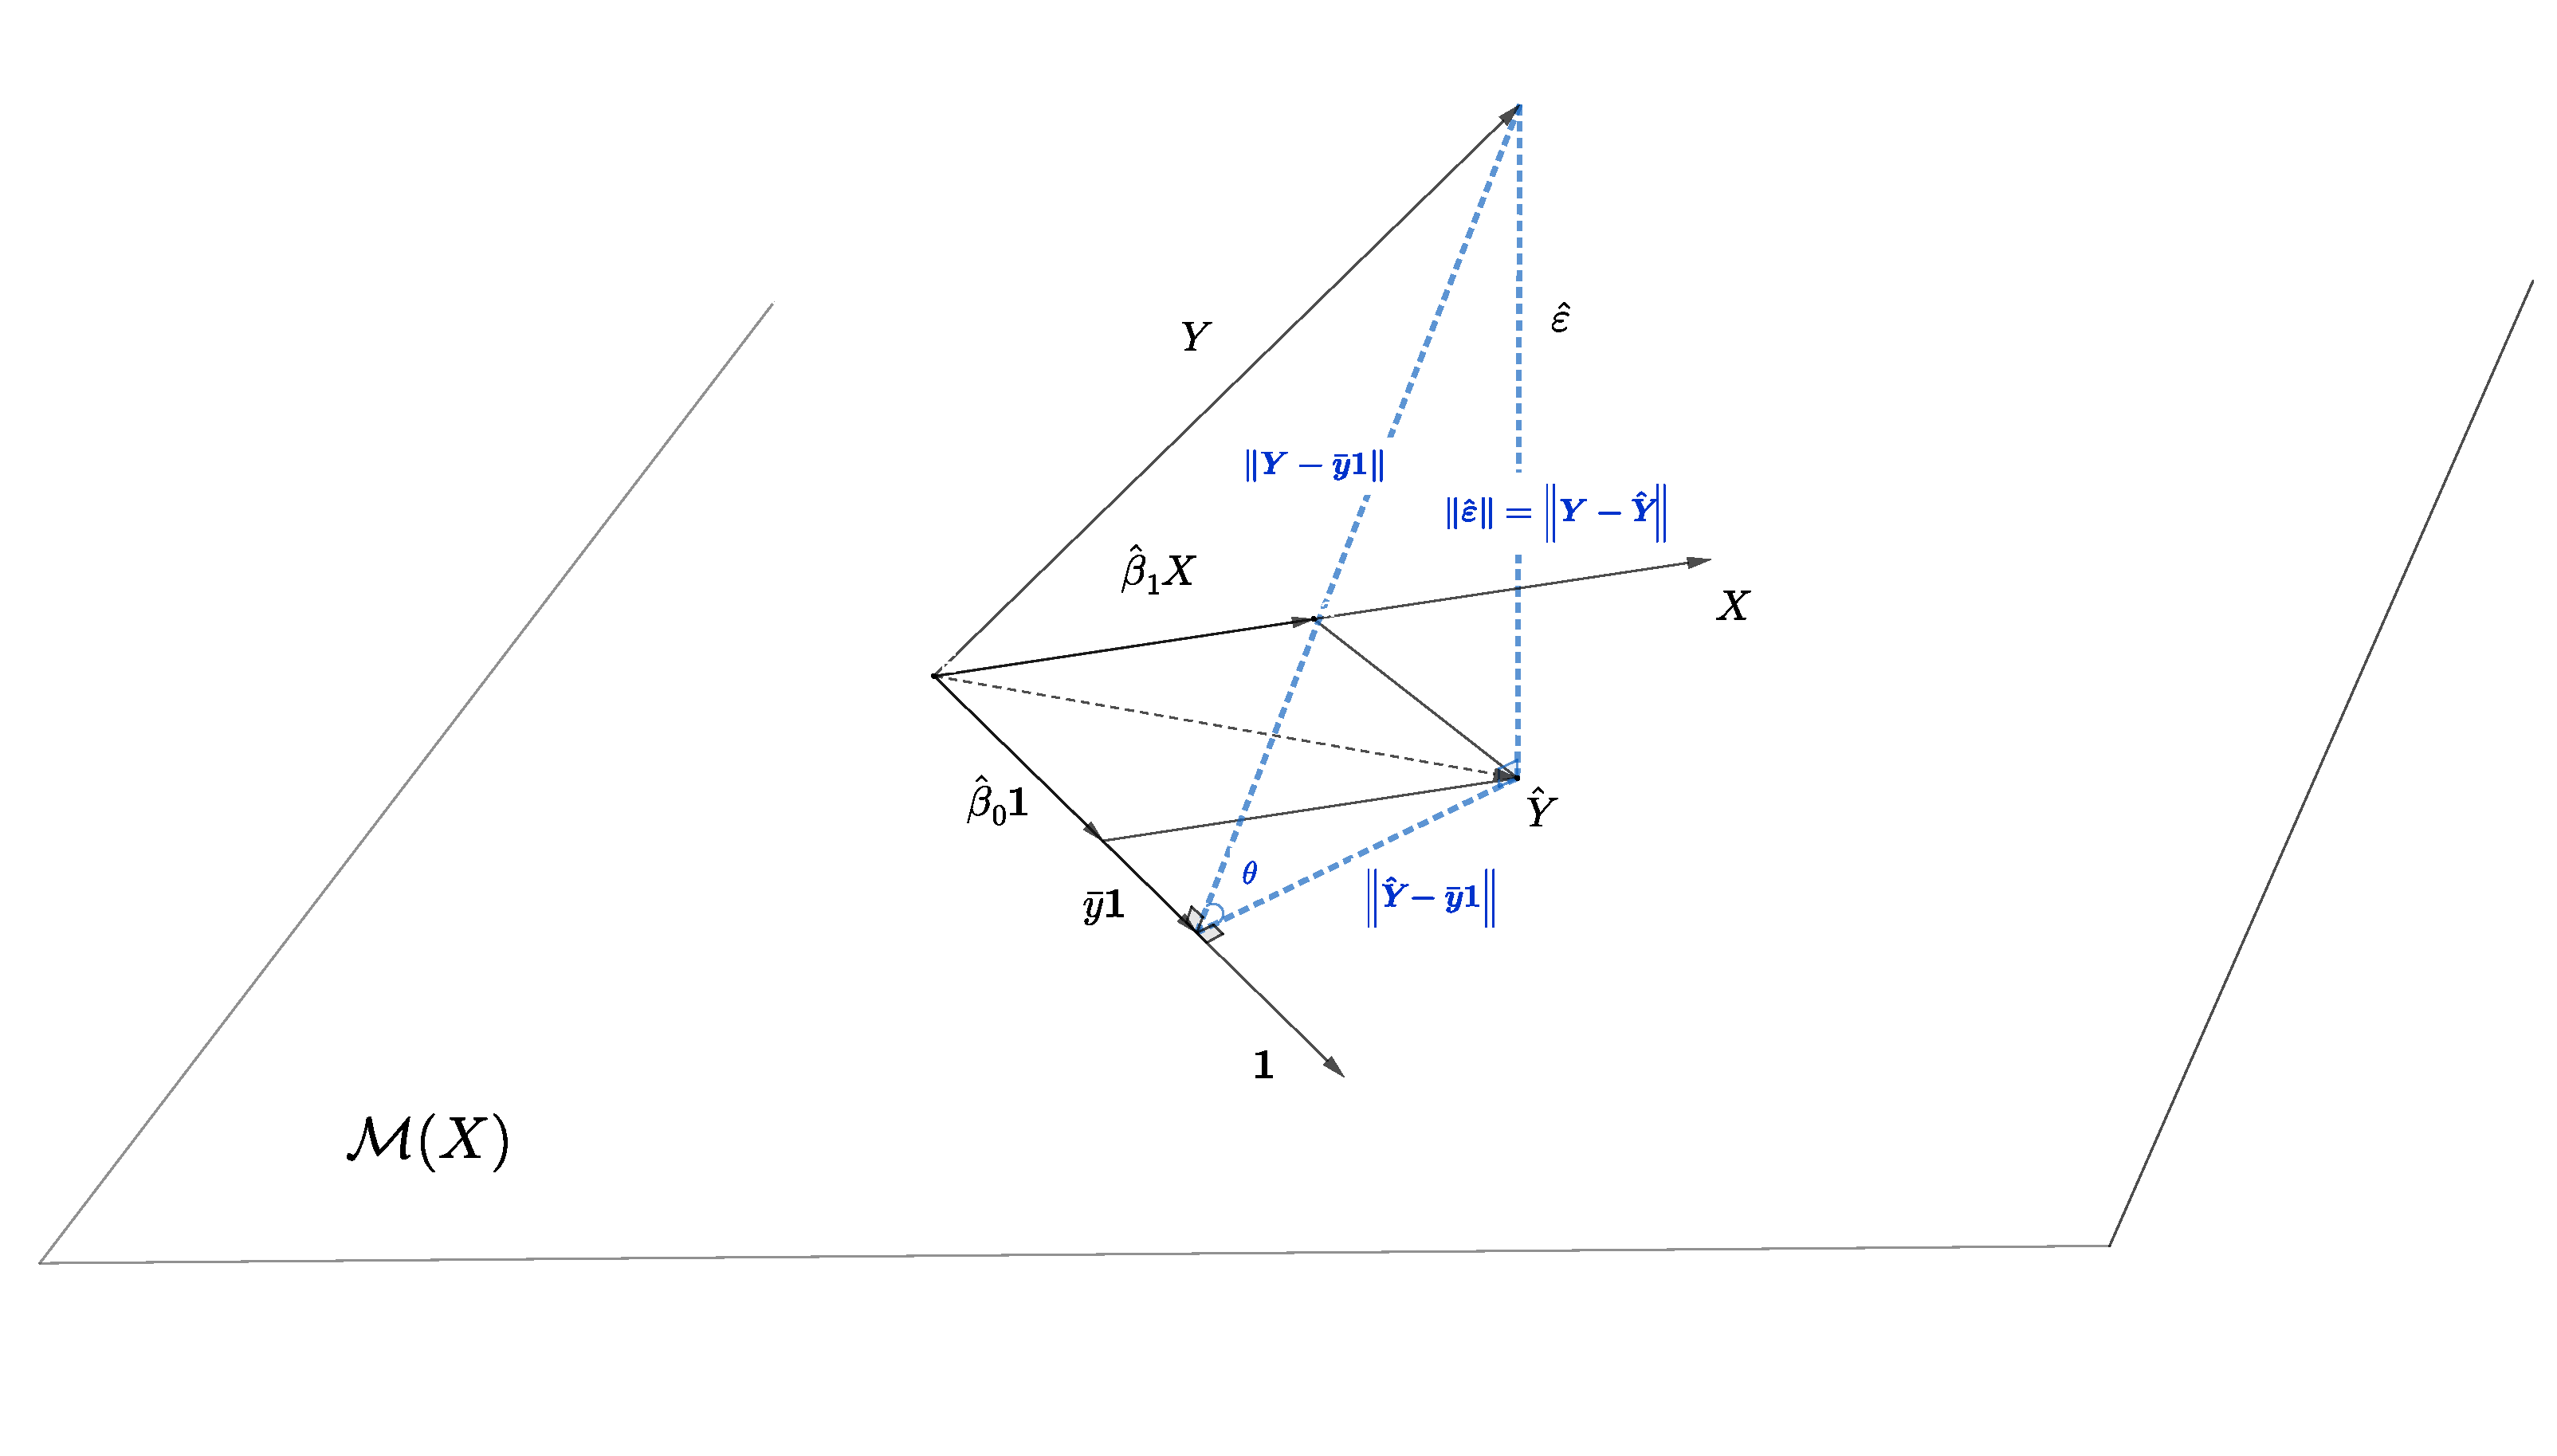
\includegraphics[width=0.8\linewidth]{images/sem2/reg_int_geom5} \end{center}

Observăm că, în general, vectorii \(\{\mathbf{1}, X\}\) nu formează o
bază ortogonală în \(\mathcal{M}(X)\) (cu excepția cazului în care
\(\langle \mathbf{1}, X\rangle = n\bar x = 0\)) prin urmare
\(\hat\beta_0\mathbf{1}\) nu este proiecția ortogonală a lui \(Y\) pe
\(\mathbf{1}\) (aceasta este
\(\frac{\langle Y, \mathbf{1}\rangle}{\lVert \mathbf{1}\rVert^2}\mathbf{1} = \bar y\mathbf{1}\))
iar \(\hat\beta_1 X\) nu este proiecția ortogonală a lui \(Y\) pe \(X\)
(aceasta fiind \(\frac{\langle Y, X\rangle}{\lVert X\rVert^2}X\)).

Fie
\(\hat\varepsilon = Y - \hat Y = (\hat\varepsilon_1, \hat\varepsilon_2, \ldots, \hat\varepsilon_n)^\intercal\)
vectorul valorilor reziduale. Aplicând Teorema lui Pitagora (în
triunghiul albastru) rezultă (descompunerea ANOVA pentru regresie) că

\begin{align*}
  \left\lVert Y - \bar y \mathbf{1}\right\rVert^2 &= \left\lVert \hat Y - \bar y \mathbf{1}\right\rVert^2 + \left\lVert \underbrace{\hat\varepsilon}_{Y - \hat Y}\right\rVert^2\\
  \sum_{i = 1}^{n}(y_i - \bar y)^2 &= \sum_{i = 1}^{n}(\hat y_i - \bar y)^2 + \sum_{i = 1}^{n}(\underbrace{\hat\varepsilon_i}_{y_i - \hat y_i})^2\\
  SS_T &= SS_{reg} + RSS
\end{align*}

Din definiția coeficientului de determinare \(R^2\) avem că

\[
R^2 = \frac{SS_{reg}}{SS_T} = \frac{\left\lVert \hat Y - \bar y \mathbf{1}\right\rVert^2}{\left\lVert Y - \bar y \mathbf{1}\right\rVert^2} = 1 - \frac{\left\lVert \hat \varepsilon\right\rVert^2}{\left\lVert Y - \bar y \mathbf{1}\right\rVert^2}
\]

și conform figurii de mai sus \(R^2 = \cos^2(\theta)\). Prin urmare dacă
\(R^2 = 1\), atunci \(\theta = 0\) și \(Y\in\mathcal{M}(X)\), deci
\(y_i = \beta_0 + \beta_1 x_i\), \(i\in\{1,2,\ldots,n\}\) (punctele
eșantionului sunt perfect aliniate) iar dacă \(R^2 = 0\), deducem că
\(\sum_{i = 1}^{n}(\hat y_i - \bar y)^2 = 0\), deci
\(\hat y_i = \bar y\) (modelul liniar nu este adaptat în acest caz, nu
putem explica mai bine decât media).

\begin{rmdexercise}
\marginnote{\enonce{13001}{}}\vspace{-7mm}

Arătați că

\[
  R^2 = r_{xy}^2 = r_{y\hat y}^2
\]

unde \(r_{xy}\) este coeficientul de corelație empiric dintre \(x\) și
\(y\).
\end{rmdexercise}

Din definiția coeficientului de determinare și folosind coeficienții
\(\hat\beta_0 = \bar y - \hat\beta_1 \bar x\) și
\(\hat\beta_1 = \frac{\sum_{i = 1}^{n}(x_i - \bar x)(y_i - \bar y)}{\sum_{i = 1}^{n}(x_i - \bar x)^2}\)
obținuți prin metoda celor mai mici pătrate avem

\begin{align*}
R^2 &= \frac{\left\lVert \hat Y - \bar y \mathbf{1}\right\rVert^2}{\left\lVert Y - \bar y \mathbf{1}\right\rVert^2} = \frac{\sum_{i = 1}^{n}(\hat\beta_0 + \hat\beta_1 x_i - \bar y)^2}{\sum_{i = 1}^{n}(y_i - \bar y)^2} = \frac{\sum_{i = 1}^{n}(\bar y - \hat\beta_1 \bar x + \hat\beta_1\bar x - \bar y)^2}{\sum_{i = 1}^{n}(y_i - \bar y)^2}\\
  &= \frac{\hat\beta_1^2\sum_{i = 1}^{n}(x_i - \bar x)^2}{\sum_{i = 1}^{n}(y_i - \bar y)^2} = \left(\frac{\sum_{i = 1}^{n}(x_i - \bar x)(y_i - \bar y)}{\sum_{i = 1}^{n}(x_i - \bar x)^2}\right)^2\frac{\sum_{i = 1}^{n}(x_i - \bar x)^2}{\sum_{i = 1}^{n}(y_i - \bar y)^2}\\
  & = \frac{\left[\sum_{i = 1}^{n}(x_i - \bar x)(y_i - \bar y)\right]^2}{\sum_{i = 1}^{n}(x_i - \bar x)^2\sum_{i = 1}^{n}(y_i - \bar y)^2} = r_{xy}^2.
\end{align*}

Pentru a verifica a doua parte, \(R^2 = r_{y\hat y}^2\), să observăm că

\[
r_{y\hat y}^2 = \frac{\left[\sum_{i = 1}^{n}(\hat y_i - \bar{\hat y})(y_i - \bar y)\right]^2}{\sum_{i = 1}^{n}(\hat y_i - \bar{\hat y})^2\sum_{i = 1}^{n}(y_i - \bar y)^2}
\]

iar
\(\bar{\hat y} = \frac{\sum_{i = 1}^{n}\hat y_i}{n} = \hat \beta_0 + \hat\beta_1 \bar x = \bar y\),
prin urmare

\[
r_{y\hat y}^2 = \frac{\left[\sum_{i = 1}^{n}(\hat y_i - \bar{y})(y_i - \bar y)\right]^2}{\sum_{i = 1}^{n}(\hat y_i - \bar{y})^2\sum_{i = 1}^{n}(y_i - \bar y)^2}.
\]

De asemenea

\begin{align*}
\sum_{i = 1}^{n}(\hat y_i - \bar{y})(y_i - \bar y) &= \sum_{i = 1}^{n}(\hat y_i - \bar{y})(y_i - \hat y_i + \hat y_i - \bar y) \\
 &= \sum_{i = 1}^{n}(\hat y_i - \bar{y})(y_i - \hat y_i) + \sum_{i = 1}^{n}(\hat y_i - \bar{y})^2
\end{align*}

și cum

\begin{align*}
\sum_{i = 1}^{n}(\hat y_i - \bar{y})(y_i - \hat y_i) &= \sum_{i = 1}^{n}(\hat \beta_0 + \hat\beta_1 x_i - \bar{y})(y_i - \hat \beta_0 - \hat\beta_1 x_i) \\
  &= \sum_{i = 1}^{n}(\bar y - \hat\beta_1 \bar x + \hat\beta_1 x_i - \bar{y})[(y_i - \bar y ) - \hat\beta_1 (x_i - \bar x)]\\
  &= \hat\beta_1 \sum_{i = 1}^{n}(x_i - \bar x)(y_i - \bar y) - \hat\beta_1^2 \sum_{i = 1}^{n}(x_i - \bar x)^2 \\
  &= \underbrace{\frac{S_{xy}}{S_{xx}}}_{\hat\beta_1}S_{xy} - \frac{S_{xy}^2}{S_{xx}^2}S_{xx} = 0
\end{align*}

deducem că
\(r_{y\hat y}^2 = \frac{\sum_{i = 1}^{n}(\hat y_i - \bar{y})^2}{\sum_{i = 1}^{n}(y_i - \bar y)^2} = R^2\).

\subsection{Aplicații numerice}\label{aplicatii-numerice}

\begin{rmdexercise}
\marginnote{\enonce{14001}{}}\vspace{-7mm}

Tabelul de mai prezintă o serie de date privind greutatea taților și
respectiv a fiului lor cel mare

\[
\begin{array}{lcccccccccccc}
  Tata: & 65 & 63 & 67 & 64 & 68 & 62 & 70 & 66 & 68 & 67 & 69 & 71\\
  Fiu: & 68 & 66 & 68 & 65 & 69 & 66 & 68 & 65 & 71 & 67 & 68 & 70
\end{array}
\]

Obținem următoarele rezultate numerice

\[
  \sum_{i = 1}^{12}t_i = 800 \quad \sum_{i = 1}^{12}t_i^2 = 53418 \quad \sum_{i = 1}^{12}t_i f_i = 54107 \quad \sum_{i = 1}^{12}f_i = 811 \quad \sum_{i = 1}^{12}f_i^2 = 54849.
\]

\begin{enumerate}
\def\labelenumi{\arabic{enumi}.}
\item
  Determinați dreapta obținută prin metoda celor mai mici pătrate a
  greutății fiilor în funcie de greutatea taților.
\item
  Determinați dreapta obținută prin metoda celor mai mici pătrate a
  greutății taților în funcie de greutatea fiilor.
\item
  Arătați că produsul pantelor celor două drepte este egal cu pătratul
  coeficientului de corelație empirică dintre \(t_i\) și \(f_i\) (sau
  coeficientul de determinare).
\end{enumerate}
\end{rmdexercise}

\begin{enumerate}
\def\labelenumi{\arabic{enumi}.}
\tightlist
\item
  Dreapta de regresie a greutății fiilor în funcție de greutatea taților
  este \(f = \hat\alpha_0 + \hat\alpha_1 t\) unde coeficienții sunt dați
  de
\end{enumerate}

\[
  \hat\alpha_0 = \bar f - \hat\alpha_1 \bar t, \quad \hat\alpha_1 = \frac{\sum_{i = 1}^{12}(t_i - \bar t)(f_i - \bar f)}{\sum_{i = 1}^{12}(t_i - \bar t)^2}
\]

Pentru datele din problema noastră coeficienții sunt
\(\hat\alpha_0 = 35.8\) și \(\hat\alpha_1 = 0.48\) iar dreapta de
regresie este \(f = 35.8 + 0.48 t\) (a se vedea figura din stânga).

\begin{enumerate}
\def\labelenumi{\arabic{enumi}.}
\setcounter{enumi}{1}
\tightlist
\item
  Dreapta de regresie a greutății taților în funcție de greutatea fiilor
  este \(t = \hat\beta_0 + \hat\beta_1 f\) unde coeficienții sunt dați
  de
\end{enumerate}

\[
  \hat\beta_0 = \bar t - \hat\beta_1 \bar f, \quad \hat\beta_1 = \frac{\sum_{i = 1}^{12}(f_i - \bar f)(t_i - \bar t)}{\sum_{i = 1}^{12}(f_i - \bar f)^2}
\]

În cazul problemei, coeficienții sunt \(\hat\beta_0 = -3.38\) și
\(\hat\beta_1 = 1.03\) iar dreapta de regresie este
\(t = -3.38 + 1.03 f\) (a se vedea figura din mijloc).

\begin{enumerate}
\def\labelenumi{\arabic{enumi}.}
\setcounter{enumi}{2}
\tightlist
\item
  Produsul pantelor celor două drepte este
\end{enumerate}

\[
\hat \alpha_1 \hat\beta_1 = \frac{\left[\sum_{i = 1}^{12}(f_i - \bar f)(t_i - \bar t)\right]^2}{\sum_{i = 1}^{12}(f_i - \bar f)^2\sum_{i = 1}^{12}(t_i - \bar t)^2}
\]

și conform \protect\hyperlink{reg_sim_ex_2}{exercițiului 2} și a
definiției coeficientului de determinare avem

\[
\hat \alpha_1 \hat\beta_1 = r_{f,t}^2= R^2.
\]

\begin{center}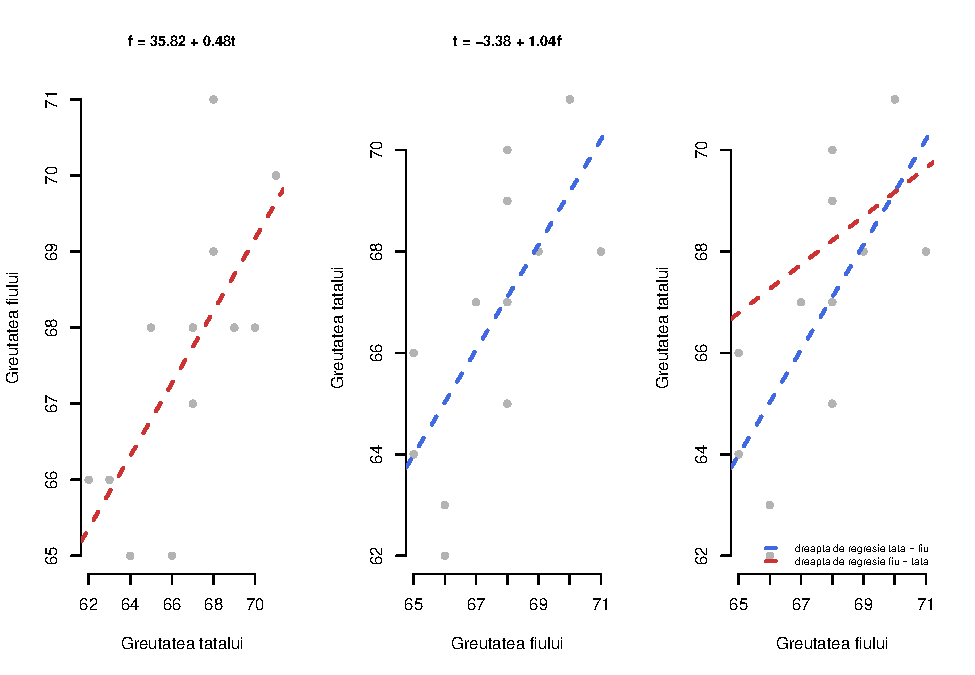
\includegraphics[width=0.9\linewidth]{Sem_2_files/figure-latex/unnamed-chunk-12-1} \end{center}

\begin{rmdexercise}
\marginnote{\enonce{14002}{}}\vspace{-7mm}

Dorim să exprimăm înălțimea \(y\) (măsurată în picioare) a unui arbore
în funcție de diametrul său \(x\) (exprimat în centimetri) la înălțimea
de 1m30 de la sol. Pentru aceasta dispunem de 20 de măsurători
\((x_i,y_i)=\)(diametru, înălțime) și în urma calculelor am obținut
rezultatele următoare: \(\bar x = 4.53\), \(\bar y = 8.65\) și

\[
\frac{1}{20}\sum_{i = 1}^{20}(x_i - \bar x)^2 = 10.97 \quad \frac{1}{20}\sum_{i = 1}^{20}(y_i - \bar y)^2 = 2.24 \quad \frac{1}{20}\sum_{i = 1}^{20}(x_i - \bar x)(y_i - \bar y) = 3.77.
\]

\begin{enumerate}
\def\labelenumi{\arabic{enumi}.}
\item
  Notăm cu \(y = \hat \beta_0 + \hat \beta_1 x\) dreapta de regresie.
  Calculați coeficienții \(\hat \beta_0\) și \(\hat \beta_1\).
\item
  Dați și calculați o măsură care descrie calitatea concordanței datelor
  cu modelul propus.
\item
  Să presupunem că abaterile standard pentru estimatorii
  \(\hat \beta_0\) și \(\hat \beta_1\) sunt \(\hat \sigma_0 = 1.62\) și
  respectiv \(\hat \sigma_1 = 0.05\). Presupunem că erorile
  \(\varepsilon_i\) sunt variabile aleatoare independente repartizare
  normal de medie \(0\) și varianțe egale. Vrem să testăm ipotezele
  \(H_0:\, \beta_j = 0\) versus \(H_1:\, \beta_j \neq 0\) pentru
  \(j = 0,1\). De ce acest test este interesant în contextul problemei
  noastre?
\end{enumerate}
\end{rmdexercise}

\begin{enumerate}
\def\labelenumi{\arabic{enumi}.}
\tightlist
\item
  Estimatorii coeficienților dreptei de regresie
  \(y = \hat \beta_0 + \hat \beta_1 x\) sunt dați de
\end{enumerate}

\[
  \hat \beta_1 = \frac{\sum_{i = 1}^{n}(x_i - \bar x)(y_i - \bar y)}{\sum_{i = 1}^{n}(x_i - \bar x)^2} \approx 0.344
\]

și respectiv

\[
  \hat \beta_0 = \bar y - \hat \beta_1 \bar x \approx 7.09
\]

\begin{enumerate}
\def\labelenumi{\arabic{enumi}.}
\setcounter{enumi}{1}
\tightlist
\item
  Pentru a măsura calitatea concordanței datelor la modelul de regresie
  vom folosi coeficientul de determinare \(R^2\). Am văzut că acesta
  corespunde pătratului coeficientului de corelație empirică:
\end{enumerate}

\[
  R^2 = r_{x,y}^2 = \left(\frac{\sum_{i = 1}^{n}(x_i - \bar x)(y_i - \bar y)}{\sqrt{\sum_{i = 1}^{n}(x_i - \bar x)^2}\sqrt{\sum_{i = 1}^{n}(y_i - \bar y)^2}}\right)^2 \approx 0.58.
\]

Observăm că modelul de regresie liniară simplă explică un pic mai mult
de jumătate din variabilitatea datelor.

\begin{enumerate}
\def\labelenumi{\arabic{enumi}.}
\setcounter{enumi}{2}
\tightlist
\item
  Sub ipoteza modelului condiționat normal (erorile \(\varepsilon_i\)
  sunt variabile aleatoare independente repartizare normal de medie
  \(0\) și varianțe egale) avem că
  \(\hat\beta_j\sim\mathcal{N}(\beta_j, \sigma_{\hat\beta_j}^2)\) și
  înlocuind varianțele \(\sigma_{\hat\beta_j}^2\) cu estimatorii
  \(\hat\sigma_j^2\), deducem că
  \(\frac{\hat\beta_j - \beta_j}{\hat\sigma_j}\sim t_{n-2}\).
\end{enumerate}

Prin urmare, sub \(H_0\) avem că

\[
\frac{\hat\beta_0}{\hat\sigma_0}\sim t_{18},
\]

iar pentru un prag de semnificație \(1-\alpha = 95\%\), ținând seama că
\(\left|\frac{\hat\beta_0}{\hat\sigma_0}\right|\approx 4.38\) și că
\(t_{18}(1-\alpha/2)\approx 2.1\), concluzionăm că respingem ipoteza
nulă.

În mod similar, pentru \(\hat\beta_1\) găsim că

\[
\left|\frac{\hat\beta_1}{\hat\sigma_1}\right|\approx 6.88 > 2.1
\]

de unde respingem ipoteza nulă \(H_0:\, \beta_1 = 0\) în acest caz de
asemenea.

\begin{center}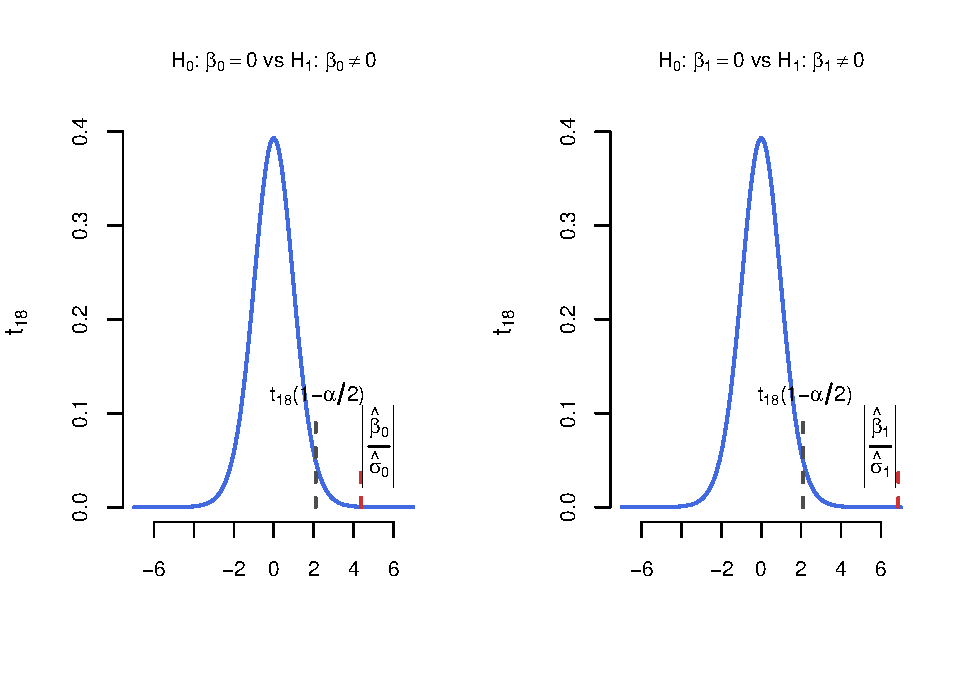
\includegraphics[width=0.9\linewidth]{Sem_2_files/figure-latex/unnamed-chunk-14-1} \end{center}

\section{Regresie liniară multiplă}\label{regresie-liniara-multipla}

Principiul problemei de regresie este de a modela o variabilă \(y\),
numită variabilă răspuns sau variabilă dependentă (cea pe care vrem să o
explicăm), cu ajutorul unei funcții care depinde de un anumit număr de
variabile \(\boldsymbol x = (x_1,\ldots, x_p)^\intercal\), numite
variabile explicative sau predictori sau independente (vom folosi în
general primele două denumiri)

\[
  y\approx g(\boldsymbol x) = g(x_1,\ldots, x_p).
\] Astfel având dat un eșantion de talie \(n\) de \((p+1)\)-upluri
\((\boldsymbol x, y)\), \(n>p\), ne propunem să determinăm \(g\).
Aproximarea, \(\approx\), din relația anterioară se poate descrie
matematic sub forma

\[
  g = \underset{f\in\mathcal{G}}{\arg\min}\sum_{i = 1}^{n}L\left(y_i - f(\boldsymbol x_i)\right)
\]

unde \(L(\cdot)\) se numește funcție de cost sau de pierdere iar
\(\mathcal{G}\) este o clasă de funcții dată.

În general funcția de cost poate lua multe forme, e.g.
\href{https://en.wikipedia.org/wiki/Loss_function}{Loss function}, dar
de cele mai multe ori vom întâlni două: funcția de cost absolut
\(L(x) = |x|\) sau funcția de cost pătratic \(L(x) = x^2\).

În ceea ce privește clasa de funcții \(\mathcal{G}\) vom considera
funcțiile liniare

\[
\mathcal{G} = \left\{f:\mathbb{R}^p\to \mathbb{R}\,|\, f(\boldsymbol x) = \begin{pmatrix}1 & \boldsymbol x\end{pmatrix} \boldsymbol \beta = \beta_0 + \beta_1 x_1 +\cdots + \beta_p x_p\right\}.
\]

Atunci când vorbim de regresie liniară ne referim la liniaritatea în
parametrii \(\beta_j\) și nu în variabilele explicative, e.g.
\(f_1(x_1,x_2) = \beta_0 + \beta_1 x_1 + \beta_2 x_2\),
\(f_2(x_1, x_2) = \beta_0 + \beta_1 x_1 + \beta_2 x_2 + \beta_3 \underbrace{x_1 x_2}_{x_3}\)
sau
\(f_3(x_1, x_2) = \beta_0 + \beta_1 x_1 + \beta_2 x_2 + \beta_3 \underbrace{x_1 x_2}_{x_3}+ \beta_4 \underbrace{x_1^2}_{x_4}+ \beta_5 \underbrace{x_2^3}_{x_5}\)
sunt toate funcții liniare în \(\boldsymbol\beta\).

\begin{center}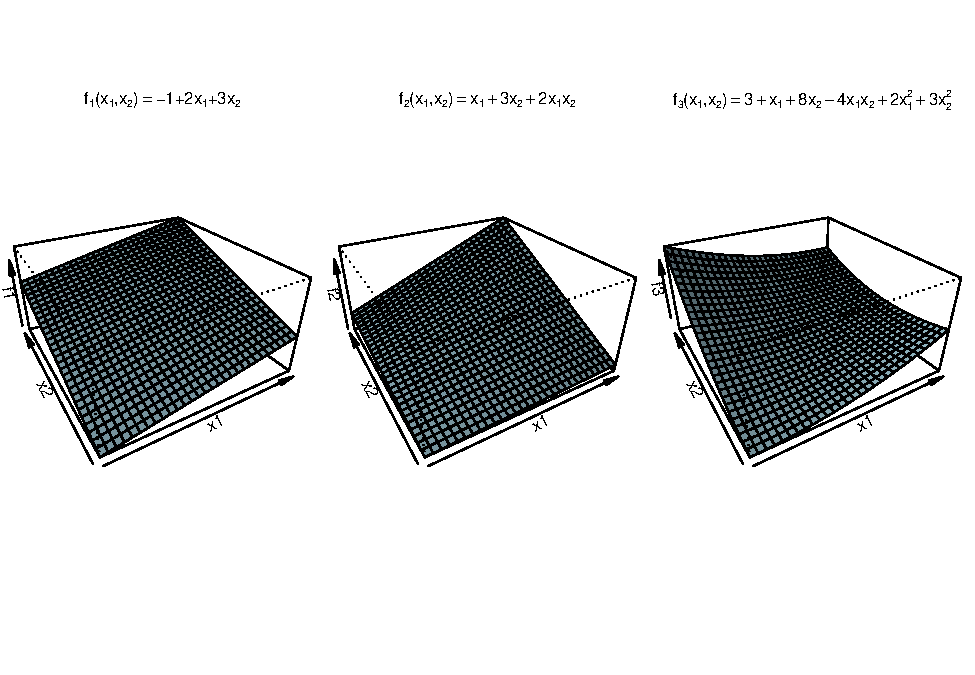
\includegraphics[width=0.85\linewidth]{Sem_2_files/figure-latex/unnamed-chunk-15-1} \end{center}

\subsection{Modelare}\label{modelare}

Modelul de regresie liniară multiplă reprezintă o extensie a modelului
de regresie liniară simplă atunci când numărul variabilelor explicative
este finit (pentru mai multe detalii privind analiza de regresie se pot
consulta monografiile \citep{Seber2003}, \citep{Weisberg2014} sau
\citep{Faraway2015}). Presupunem că datele verifică modelul

\[
  y_i = \beta_0 + \beta_1 x_{i1} + \cdots + \beta_p x_{ip} + \varepsilon_i, \quad i = 1,2,\ldots,n
\] unde

\begin{itemize}
\item
  \(x_{ij}\) sunt valori cunoscute și nu sunt aleatoare
\item
  parametrii \(\beta_j\) sunt necunoscuți și nu sunt aleatori
\item
  \(\varepsilon_i\) sunt variabile aleatoare necunoscute
\end{itemize}

Scris sub formă compactă modelul devine

\[
  \boldsymbol Y = \boldsymbol X\boldsymbol \beta + \boldsymbol \varepsilon
\]

unde

\begin{itemize}
\tightlist
\item
  \(\mathbf{X}\) se numește \emph{matricea de design}
\end{itemize}

\[
\mathbf{X}=\begin{pmatrix}
1 & x_{11} & \cdots & x_{1p}\\
\vdots & \vdots & \ddots & \vdots\\
1 & x_{n1} & \cdots & x_{np}
\end{pmatrix}_{n\times(p+1)}
\]

\begin{itemize}
\tightlist
\item
  \(\mathbf{Y}\) este \emph{vectorul răspuns} și este un vector aleator,
  \(\boldsymbol\beta\) este \emph{vectorul parametrilor} sau
  coeficienților și este necunoscut iar \(\boldsymbol\varepsilon\) este
  \emph{vectorul erorilor} și este un vector aleator
\end{itemize}

\[
\mathbf{Y}=\begin{pmatrix}
Y_1 \\
\vdots \\
Y_n
\end{pmatrix}_{n\times 1},\quad\boldsymbol\beta=\begin{pmatrix}
\beta_0 \\
\beta_1 \\
\vdots \\
\beta_p
\end{pmatrix}_{(p+1)\times 1}\text{ și }\quad
\boldsymbol\varepsilon=\begin{pmatrix}
\varepsilon_1 \\
\vdots \\
\varepsilon_n
\end{pmatrix}_{n\times 1}.
\]

Ipotezele modelului de regresie liniară multiplă sunt:

\[
  \begin{array}{ll}
    \mathcal{H}_1: \, rang(\boldsymbol X) = p+1\\
    \mathcal{H}_2: \, \mathbb{E}[\boldsymbol \varepsilon] = 0,\, Var(\boldsymbol \varepsilon) = \sigma^2 I_n
  \end{array}
\]

Prima ipoteză ne spune că matricea de design \(\boldsymbol X\) are
coloanele liniar independente iar a doua ipoteză se referă la
centralitatea erorilor (medie nulă), homoscedasticitatea (aceeași
varianță) și necorelarea acestora.

\subsection{Metoda celor mai mici
pătrate}\label{metoda-celor-mai-mici-patrate}

În această secțiune vom prezenta estimatorul lui \(\boldsymbol \beta\)
obținut prin metoda celor mai mici pătrate, metodă care folosește ca
funcție de cost \(L\) funcția \(L(x) = x^2\). Estimatorul
\(\hat{\boldsymbol \beta}\) obținut prin metoda celor mai mici pătrate
este definit prin

\[
  \hat{\boldsymbol \beta} = \underset{\boldsymbol\beta\in\mathbb{R}^{p+1}}{\arg\min}\sum_{i = 1}^{n}\left[y_i - \left(\beta_0 + \beta_1 x_{i1} + \cdots + \beta_p x_{ip}\right)\right]^2 = \underset{\boldsymbol\beta\in\mathbb{R}^{p+1}}{\arg\min}\sum_{i = 1}^{n}\left(y_i - \sum_{j= 0}^{p}\beta_j x_{ij}\right)^2 = \underset{\boldsymbol\beta\in\mathbb{R}^{p+1}}{\arg\min}\left\lVert \boldsymbol Y - \boldsymbol X \boldsymbol\beta\right\rVert^2
\]

unde am folosit convenția \(x_{i0} = 1\), \(i = 1,2,\ldots,n\).

\begin{rmdexercise}
\marginnote{\enonce{22001}{}}\vspace{-7mm}

Arătați că dacă ipoteza \(\mathcal{H}_1\) este adevărată atunci
estimatorul \(\hat{\boldsymbol \beta}\) obținut prin metoda celor mai
mici pătrate este

\[
  \hat{\boldsymbol \beta} = (\boldsymbol{X}^\intercal \boldsymbol X)^{-1}\boldsymbol{X}^\intercal \boldsymbol Y
\]
\end{rmdexercise}

Ne propunem să prezentăm mai multe metode de calcul pentru estimatorul
\(\hat{\boldsymbol \beta}\).

\begin{enumerate}
\def\labelenumi{\alph{enumi})}
\tightlist
\item
  Metoda geometrică
\end{enumerate}

Din punct de vedere geometric, ne plasăm în spațiul variabilelor
\(\mathbb{R}^n\) (am presupus că \(n>p\))). Vectorul variabilelor
răspuns \(\boldsymbol Y\in \mathbb{R}^n\) iar matricea de design
\(\boldsymbol{X}\) poate fi văzută ca fiind formată din \(p+1\) vectori
coloană,
\(\boldsymbol{X} = \left[\underbrace{\boldsymbol X_0}_{\mathbf{1} = (1,\cdots,1)}|\boldsymbol X_1|\cdots|\boldsymbol X_p\right]\).

Începem prin a reaminti câteva noțiuni de algebră liniară, pentru mai
multe detalii se poate consulta monografia \citep{Turtoi2000}. Fiind
dată matricea (de design)
\(\boldsymbol{X}\in\mathcal{M}_{n,p+1}(\mathbb{R})\) putem defini
nucleul matricei

\[
\ker(\boldsymbol{X}) = \left\{\boldsymbol u\in\mathbb{R}^{p+1}\,|\, \boldsymbol{X}\boldsymbol u = 0\right\}
\]

ca fiind subspațiul lui \(\mathbb{R}^{p+1}\) care conține vectorii
ortogonali pe liniile din matricea \(\boldsymbol{X}\). De asemenea,
imaginea matricei \(\boldsymbol{X}\) este subspațiul vectorilor din
\(\mathbb{R}^n\) care se pot scrie ca o combinație liniară de coloanele
matricei \(\boldsymbol{X}\) și este definit prin

\[
\mathrm{Im}(\boldsymbol{X}) = \left\{\boldsymbol v\in\mathbb{R}^{n}\,|\,\exists \boldsymbol u\in\mathbb{R}^{p+1} \text{ a.î. } \boldsymbol{X}\boldsymbol u = \boldsymbol v\right\}.
\]

Se poate arăta (a se vedea \citep[Capitolul 1]{Turtoi2000}) că
\(\dim \ker(\boldsymbol{X}) = p + 1 - \mathrm{rang}(\boldsymbol{X})\) și
că \(\dim \mathrm{Im}(\boldsymbol{X}) = \mathrm{rang}(\boldsymbol{X})\)
ceea ce conduce la
\(\dim \ker(\boldsymbol{X}) + \dim \mathrm{Im}(\boldsymbol{X}) = p+1\)
(caz particular al \emph{teoremei lui Grassman}).

Reamintim că doi vectori \(\boldsymbol u\) și \(\boldsymbol v\) sunt
ortogonali dacă \(\langle \boldsymbol u, \boldsymbol v\rangle = 0\), iar
în acest caz scriem \(\boldsymbol u \perp \boldsymbol v\), și că două
subspații \(V\) și \(W\) sunt ortogonale dacă
\(\forall \boldsymbol v \in V\) și respectiv
\(\forall \boldsymbol w \in W\) avem
\(\boldsymbol v\perp \boldsymbol w\) și notăm \(V\perp W\). De asemenea,
spațiul ortogonal al lui \(V\) este spațiul \(V^{\perp}\) care conține
toți vectorii ortogonali pe \(V\) și are ca proprietăți:
\(V\cap V^{\perp} = \{0\}\) și \(\left(V^{\perp}\right)^\perp = V\). Se
poate arăta cu ușurință că dacă \(V\) este un subspațiu a lui
\(W\subset\mathbb{R}^n\) atunci pentru orice vector
\(\boldsymbol w\in W\) avem că
\(\boldsymbol w = \boldsymbol v + \boldsymbol v^\perp\) unde
\(\boldsymbol v\in V\) și \(\boldsymbol v^\perp\in V^\perp\) iar
descompunerea se face în mod unic (acest rezultat se mai scrie și sub
forma \(W = V\oplus V^\perp\)). Se numește \emph{proiecție
ortogonală}\footnote{În general, numim \emph{proiecție} un endomorfism
  \(p: W\to W\) cu proprietatea că există o descompunere în sumă directă
  \(W = V_1\oplus V_2\) (și spunem proiecție pe \(V_1\) de-a lungul lui
  \(V_2\)) astfel încât \(p(\boldsymbol w) = \boldsymbol v_1\),
  \(\forall \boldsymbol w\in W\) cu
  \(\boldsymbol w = \boldsymbol v_1 + \boldsymbol v_2\),
  \(\boldsymbol v_1\in V_1\) și \(\boldsymbol v_2\in V_2\).} a lui
\(\boldsymbol w\) pe \(V\) de-a lungul lui \(V^\perp\) endomorfismul
\(p_V: W\to W\) definit prin \(p_V(\boldsymbol w) = \boldsymbol v\). Se
poate arăta cu ușurință că dacă \(V\) este un subspațiu vectorial al lui
\(W\) atunci au loc următoarele proprietăți:

\begin{enumerate}
\def\labelenumi{\roman{enumi})}
\item
  pentru orice \(\boldsymbol w\in W\) avem:
  \(\boldsymbol w = p_V(\boldsymbol w) + p_{V^\perp}(\boldsymbol w)\),
  \(\lVert p_V(\boldsymbol w)\rVert \leq \lVert \boldsymbol w\rVert\)
  iar \(\boldsymbol w - p_{V}(\boldsymbol w) \perp \boldsymbol v\),
  \(\forall \boldsymbol v \in V\)
\item
  pentru orice \(\boldsymbol w\in W\) are loc
  \(\lVert \boldsymbol w - p_V(\boldsymbol w)\rVert = \inf_{\boldsymbol v\in V}\lVert \boldsymbol w - \boldsymbol v\rVert\)
\item
  dacă \(p\) este o proiecție ortogonală atunci \(p\circ p = p\)
\item
  dacă \(p\) este un endomorfism care verifică \(p\circ p = p\) și în
  plus \(\textrm{Im}(p)\perp \ker(p)\) atunci \(p\) este proiecția
  ortogonală pe \(\textrm{Im}(p)\) de-a lungul lui \(\ker(p)\)
\item
  dacă \(\{\boldsymbol e_1, \boldsymbol e_2, \ldots, \boldsymbol e_k\}\)
  este o bază ortonormală în \(V\) atunci
  \(p_V(\boldsymbol w) = \sum_{i = 1}^{k}\langle \boldsymbol w, \boldsymbol e_i\rangle \boldsymbol e_i\)
\end{enumerate}

Spunem că o matrice pătratică \(P\in\mathcal{M}_{n}(\mathbb{R})\) este o
matrice de proiecție dacă este idempotentă \(P^2 = P\) (numele vine de
la faptul că pentru \(\boldsymbol x\in\mathbb{R}^n\) aplicația liniară
\(P\boldsymbol x\) este proiecția lui \(\boldsymbol x\) pe
\(\mathrm{Im}(P)\) de-a lungul lui \(\ker(P)\) - a se vedea
\citep[Capitolul 1, Secțiunea 5.2]{Turtoi2000} sau \citep[Capitolul
2]{Yanai2011}). Dacă în plus matricea \(P\) este simetrică, i.e.
\(P = P^\intercal\), atunci \(P\boldsymbol x\) este proiecția ortogonală
a lui \(\boldsymbol x\) pe \(V = \mathrm{Im}(P)\) de-a lungul lui
\(V^\perp = \ker(P)\), cu alte cuvinte în descompunerea
\(\boldsymbol x = P\boldsymbol x + (I - P)\boldsymbol x\) vectorii
\(P\boldsymbol x\) și respectiv \((I - P)\boldsymbol x\) sunt ortogonali
\citep[Capitolul 2, Secțiunea 2.2]{Yanai2011}. Prin urmare matricea
\(P\) este o matrice de proiecție ortogonală dacă are loc relația
\(\boldsymbol v\perp \boldsymbol v - P\boldsymbol v\) adică
\(\langle\boldsymbol v, \boldsymbol v - P\boldsymbol v\rangle = 0\)
pentru toți \(\boldsymbol v\).

Dacă \(\boldsymbol{X}\in\mathcal{M}_{m,k}(\mathbb{R})\) este o matrice
de \(\mathrm{rang}(\boldsymbol{X}) = k\) (\(m\geq k\)), deci
\(\boldsymbol{X}^\intercal\boldsymbol{X}\) este inversabilă, atunci
pentru a determina matricea de proiecție ortogonală \(P_X\) pe
subspațiul imagine \(\mathrm{Im}(\boldsymbol{X})\) să observăm că dacă
\(\boldsymbol v\in \textrm{Im}(\boldsymbol X)\) atunci
\(\boldsymbol v = \boldsymbol X \boldsymbol \alpha\) și cum
\(P_X \boldsymbol v = \boldsymbol v\) deducem că
\(P_X \boldsymbol v = \boldsymbol{X}\underbrace{\left(\boldsymbol{X}^\intercal\boldsymbol{X}\right)^{-1}\boldsymbol{X}^\intercal \boldsymbol v}_{= \boldsymbol \alpha}\).
În plus dacă
\(\boldsymbol v^\perp\in \textrm{Im}(\boldsymbol X)^\perp = \ker(\boldsymbol X^\intercal)\)
atunci \(\boldsymbol X^\intercal\boldsymbol v^\perp = 0\) prin urmare
\(\boldsymbol{X}\left(\boldsymbol{X}^\intercal\boldsymbol{X}\right)^{-1}\boldsymbol{X}^\intercal \boldsymbol v^\perp = 0\)
și astfel, pentru
\(\boldsymbol w = \boldsymbol v + \boldsymbol v^\perp\) arbitrar, avem
\(P_{X}\boldsymbol w = \boldsymbol{X}\left(\boldsymbol{X}^\intercal\boldsymbol{X}\right)^{-1}\boldsymbol{X}^\intercal\boldsymbol w\)
de unde găsim că

\[
  P_{X} = \boldsymbol{X}\left(\boldsymbol{X}^\intercal\boldsymbol{X}\right)^{-1}\boldsymbol{X}^\intercal.
\]

În mod similar se arată că matricea de proiecție ortogonală pe
\(\ker(\boldsymbol{X})\) este \(P_{X\perp} = I - P_{X}\). Nu este
dificil de văzut că cele două matrice, \(P_{X}\) și respectiv
\(P_{X\perp}\), sunt idempotente. De asemenea, ținând seama că valorile
proprii ale unei matrice idempotente sunt \(0\) sau \(1\) concluzionăm
că \(\mathrm{rang}(P_X) = \mathrm{Tr}(P_X)\).

În cazul particular în care \(\boldsymbol{X} = \boldsymbol{v}\) avem

\[
  P_v = \boldsymbol{v}\left(\boldsymbol{v}^\intercal\boldsymbol{v}\right)^{-1}\boldsymbol{v}^\intercal = \frac{\boldsymbol{v}\boldsymbol{v}^\intercal}{\lVert\boldsymbol{v}\rVert^2}
\]

prin urmare proiecția vectorului \(\boldsymbol{u}\) pe
\(\boldsymbol{v}\) este
\(P_v\boldsymbol{u} = \frac{\boldsymbol{v}\boldsymbol{v}^\intercal}{\lVert\boldsymbol{v}\rVert^2}\boldsymbol{u} = \frac{\langle\boldsymbol{u}, \boldsymbol{v}\rangle}{\lVert\boldsymbol{v}\rVert^2}\boldsymbol{v}\).

Pentru problema noastră, notăm cu
\(\mathcal{M}(X) = \mathrm{Im}(\boldsymbol{X})\) subspațiul imagine și
conform ipotezei \(\mathcal{H}_1\) avem că
\(\mathrm{rang}(\boldsymbol{X}) = p+1\), deci
\(\dim \mathcal{M}(X) = p+1\). Din definiția spațiului imagine avem că
toți vectorii din \(\mathcal{M}(X)\) sunt de forma
\(\boldsymbol X \boldsymbol\alpha\), cu
\(\boldsymbol \alpha = (\alpha_0, \alpha_1,\ldots, \alpha_p)\in\mathbb{R}^{p+1}\)

\[
  \boldsymbol X \boldsymbol\alpha = \sum_{i = 0}^{p}\alpha_i \boldsymbol X_i.
\]

Conform modelului de regresie,
\(\boldsymbol Y = \boldsymbol X\boldsymbol \beta + \boldsymbol \varepsilon\),
vectorul răspuns \(\boldsymbol Y\) este suma dintre un element din
\(\mathcal{M}(X)\) și un element din \(\mathbb{R}^n\) care nu are niciun
motiv să aparțină tot lui \(\mathcal{M}(X)\). Astfel, problema
minimizării funcției
\(S(\boldsymbol \beta) = \left\lVert \boldsymbol Y - \boldsymbol X \boldsymbol\beta\right\rVert^2\)
revine la a găsi acel vector din \(\mathcal{M}(X)\) care este cel mai
aproape de \(\boldsymbol Y\) în sensul distanței euclidiene, cu alte
cuvinte de a determina vectorul proiecției ortogonale a lui
\(\boldsymbol Y\) pe \(\mathcal{M}(X)\) (a se vedea figura de mai jos).

Proiecția ortogonală a lui \(\boldsymbol Y\) pe \(\mathcal{M}(X)\) se
notează cu \(\hat{\boldsymbol Y} = P_X \boldsymbol Y\), unde \(P_X\)
este matricea de proiecție ortogonală pe \(\mathcal{M}(X)\), iar spațiul
ortogonal \(\mathcal{M}(X)^\perp\) se mai numește și spațiul
reziduurilor și are dimensiunea
\(\dim \mathcal{M}(X)^\perp = n - (p+1)\) (\emph{teorema lui Grassman}).
Să remarcăm că \(\hat{\boldsymbol Y}\in\mathcal{M}(X)\) deci putem scrie
\(\hat{\boldsymbol Y} = \boldsymbol X\hat{\boldsymbol \beta}\) unde
\(\hat{\boldsymbol \beta}\) reprezintă estimatorul obținut prin metoda
celor mai mici pătrate iar elementele lui \(\hat{\boldsymbol \beta}\)
sunt coordonatele vectorului \(\hat{\boldsymbol Y}\) în baza
\(\{\boldsymbol X_0, \boldsymbol X_1,\ldots, \boldsymbol X_p\}\) a
spațiului \(\mathcal{M}(X)\). Cum reperul
\(\{\boldsymbol X_0, \boldsymbol X_1,\ldots, \boldsymbol X_p\}\) nu este
neapărat ortogonal, elementele \(\hat{\beta_j}\) nu sunt neapărat
coordonatele proiecției lui \(\boldsymbol Y\) pe \(\boldsymbol X_j\),
aceasta din urmă fiind dată de

\begin{align*}
  P_{X_j}\boldsymbol Y &= P_{X_j}P_X \boldsymbol Y = P_{X_j}\sum_{i = 0}^{p} \hat{\beta_i}\boldsymbol X_i\\
    &= \sum_{i = 0}^{p}\hat{\beta_i} P_{X_j}\boldsymbol X_i = \hat{\beta_j} \boldsymbol X_j + \sum_{i \neq j}\hat{\beta_i} P_{X_j}\boldsymbol X_i
\end{align*}

În cazul în care \(\boldsymbol X_j\) este ortogonal pe
\(\boldsymbol X_i\), \(i\neq j\), atunci
\(P_{X_j}\boldsymbol Y = \hat{\beta_j} \boldsymbol X_j\) iar dacă
\(\langle\boldsymbol X_i, \boldsymbol X_j\rangle = 0\) pentru toți
\(i\neq j\) atunci matricea
\(\boldsymbol X^\intercal\boldsymbol X = \mathrm{diag}\left(\lVert\boldsymbol X_0\rVert^2, \lVert\boldsymbol X_1\rVert^2, \ldots, \lVert\boldsymbol X_p\rVert^2\right)\).

O altă metodă (tot prin proiecții) de a arăta că
\(\hat{\boldsymbol \beta} = (\boldsymbol{X}^\intercal \boldsymbol X)^{-1}\boldsymbol{X}^\intercal \boldsymbol Y\)
se bazează pe observația că proiecția ortogonală
\(\hat{\boldsymbol Y} = \boldsymbol X\hat{\boldsymbol \beta}\) este
definită ca fiind unicul vector pentru care
\(\boldsymbol Y - \hat{\boldsymbol Y}\) este ortogonal pe
\(\mathcal{M}(X)\). Cum \(\mathcal{M}(X)\) este generat de
\(\{\boldsymbol X_0, \boldsymbol X_1,\ldots, \boldsymbol X_p\}\) putem
spune că \(\boldsymbol Y - \hat{\boldsymbol Y}\) este ortogonal pe
fiecare \(\boldsymbol X_i\):

\[
\left\{\begin{array}{lll}
  \langle \boldsymbol X_0, \boldsymbol Y - \hat{\boldsymbol Y}\rangle = 0\\
  \langle \boldsymbol X_1, \boldsymbol Y - \hat{\boldsymbol Y}\rangle = 0\\
  \vdots\\
  \langle \boldsymbol X_p, \boldsymbol Y - \hat{\boldsymbol Y}\rangle = 0
\end{array}\right. \iff \left\{\begin{array}{lll}
  \langle \boldsymbol X_0, \boldsymbol Y - \boldsymbol X\hat{\boldsymbol \beta}\rangle = 0\\
  \langle \boldsymbol X_1, \boldsymbol Y - \boldsymbol X\hat{\boldsymbol \beta}\rangle = 0\\
  \vdots\\
  \langle \boldsymbol X_p, \boldsymbol Y - \boldsymbol X\hat{\boldsymbol \beta}\rangle = 0
\end{array}\right. \iff \boldsymbol X^\intercal \left(\boldsymbol Y - \boldsymbol X\hat{\boldsymbol \beta}\right) = 0
\]

de unde găsim \emph{sistemul de ecuații normale}

\[
\boldsymbol X^\intercal\boldsymbol X\hat{\boldsymbol \beta} = \boldsymbol X^\intercal\boldsymbol Y
\]

care, atunci când ipoteza \(\mathcal{H}_1\) este adevărată - matricea
\(\boldsymbol X^\intercal \boldsymbol X\) este inversabilă, revine la

\[
\hat{\boldsymbol \beta} = (\boldsymbol X^\intercal \boldsymbol X)^{-1} \boldsymbol X^\intercal \boldsymbol Y.
\]

\begin{center}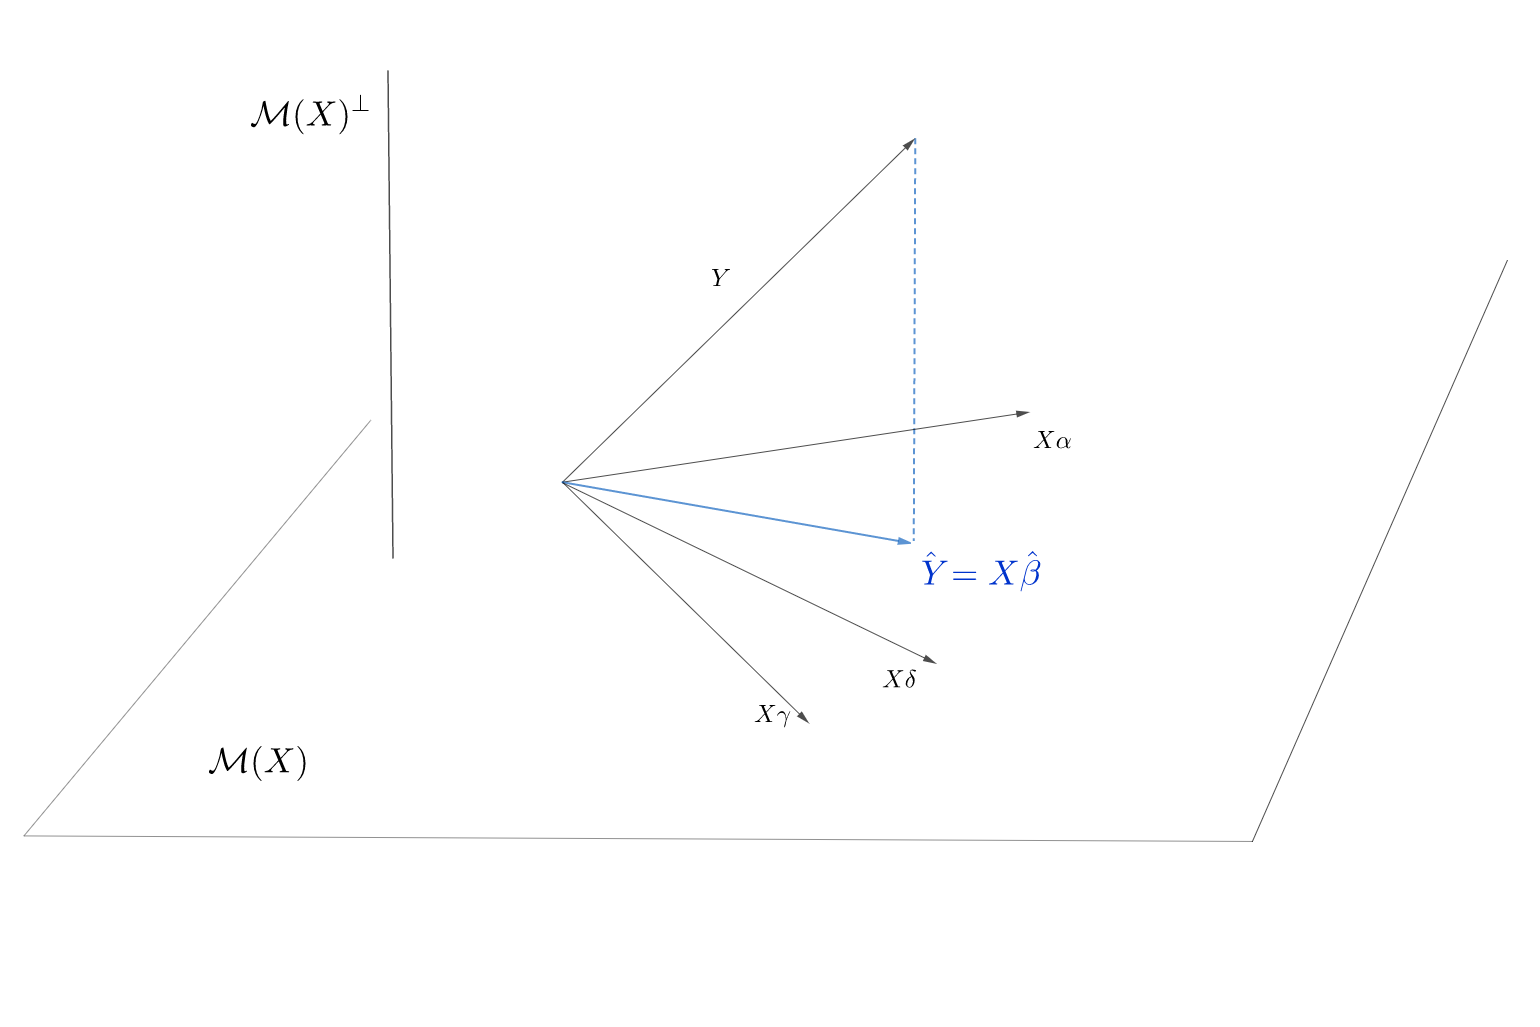
\includegraphics[width=0.8\linewidth]{images/sem2/RegMult_p1} \end{center}

Notând cu \(P_{X^\perp} = I_n - P_X\) matricea de proiecție ortogonală
pe \(\mathcal{M}^\perp(X)\), unde
\(P_X = \boldsymbol X(\boldsymbol X^\intercal \boldsymbol X)^{-1} \boldsymbol X^\intercal\)
este matricea de proiecție ortogonală pe \(\mathcal{M}(X)\), observăm că
descompunerea

\[
  \boldsymbol Y = \hat{\boldsymbol Y} + \left(\boldsymbol Y - \hat{\boldsymbol Y}\right) = P_X\boldsymbol Y + (I - P_X)\boldsymbol Y = P_X\boldsymbol Y + P_{X^\perp}\boldsymbol Y
\]

nu este altceva decât descompunerea ortogonală a lui \(\boldsymbol Y\)
pe \(\mathcal{M}(X)\) și respectiv \(\mathcal{M}^\perp(X)\). De asemenea
este de remarcat faptul că în ceea ce privește notația folosită în
literatura de statistică de specialitate, matricea de proiecție
ortogonală \(P_X\) se mai notează și cu \(H\) (care vine de la
\emph{hat}, \(\hat{\boldsymbol Y} = H\boldsymbol Y\)).

\begin{enumerate}
\def\labelenumi{\alph{enumi})}
\setcounter{enumi}{1}
\tightlist
\item
  Metoda analitică
\end{enumerate}

O a doua metodă este metoda analitică. Problema noastră cere să căutăm
vectorul \(\boldsymbol \beta\in\mathbb{R}^{p+1}\) care minimizează
funcția

\begin{align*}
S(\boldsymbol \beta) &= \left\lVert \boldsymbol Y - \boldsymbol X \boldsymbol\beta\right\rVert^2 = \left(\boldsymbol Y - \boldsymbol X \boldsymbol\beta\right)^\intercal\left(\boldsymbol Y - \boldsymbol X \boldsymbol\beta\right) = \boldsymbol Y^\intercal \boldsymbol Y - \boldsymbol Y^\intercal \boldsymbol X \boldsymbol\beta - \boldsymbol \beta^\intercal \boldsymbol X^\intercal \boldsymbol Y + \boldsymbol \beta^\intercal \boldsymbol X^\intercal \boldsymbol X \boldsymbol\beta \\
  & = \boldsymbol \beta^\intercal \boldsymbol X^\intercal \boldsymbol X \boldsymbol\beta - 2 \boldsymbol Y^\intercal \boldsymbol X \boldsymbol\beta + \lVert  \boldsymbol Y \rVert^2
\end{align*}

unde am folosit faptul că
\(\boldsymbol Y^\intercal \boldsymbol X \boldsymbol\beta = \left(\boldsymbol Y^\intercal \boldsymbol X \boldsymbol\beta\right)^\intercal = \boldsymbol \beta^\intercal \boldsymbol X^\intercal \boldsymbol Y\)
(sunt elemente de dimensiune \(1\times 1\)). Pentru aceasta trebuie să
rezolvăm ecuația \(\nabla S(\boldsymbol \beta) = 0\) și să verificăm că
soluția este într-adevăr punct de minim.

Reamintim că dacă \(f:\mathbb{R}^k\to\mathbb{R}\) atunci

\[
\nabla f = \frac{\partial f}{\partial \boldsymbol x^\intercal} = \begin{pmatrix}\frac{\partial f}{\partial x_1} & \frac{\partial f}{\partial x_2} & \cdots & \frac{\partial f}{\partial x_k}\end{pmatrix}.
\]

În particular, pentru
\(f(\boldsymbol x) = \boldsymbol a^\intercal \boldsymbol x\) (formă
liniară) avem

\[
  \nabla f = \frac{\partial \boldsymbol a^\intercal \boldsymbol x}{\partial \boldsymbol x^\intercal} = \begin{pmatrix}\frac{\partial \sum_{i=1}^{k}a_i x_i}{\partial x_1} & \frac{\partial \sum_{i=1}^{k}a_i x_i}{\partial x_2} & \cdots & \frac{\partial \sum_{i=1}^{k}a_i x_i}{\partial x_k}\end{pmatrix} = \boldsymbol a^\intercal
\]

iar
\(\frac{\partial \boldsymbol a^\intercal \boldsymbol x}{\partial \boldsymbol x} = \boldsymbol a\).

În cazul în care \(f\) este o aplicație liniară,
\(f(\boldsymbol x) = A \boldsymbol x\) unde
\(A\in\mathcal{M}_{m,k}(\mathbb{R})\), atunci

\[
  A \boldsymbol x = \begin{pmatrix}\sum_{j=1}^{k}a_{1j} x_j\\
  \sum_{j=1}^{k}a_{2j} x_j\\
  \vdots\\
  \sum_{j=1}^{k}a_{mj} x_j\end{pmatrix}, \qquad \frac{\partial A \boldsymbol x}{\partial x_j} = \begin{pmatrix}a_{1j}\\
  a_{2j}\\
  \vdots\\
  a_{mj}\end{pmatrix}
\]

și

\[
  \frac{\partial A \boldsymbol x}{\partial \boldsymbol x^\intercal} = \begin{pmatrix}\begin{pmatrix}a_{11}\\
  a_{21}\\
  \vdots\\
  a_{m1}\end{pmatrix}, \ldots, \begin{pmatrix}a_{1j}\\
  a_{2j}\\
  \vdots\\
  a_{mj}\end{pmatrix}, \ldots, \begin{pmatrix}a_{1k}\\
  a_{2k}\\
  \vdots\\
  a_{mk}\end{pmatrix}\end{pmatrix} = \begin{pmatrix}a_{11} & \cdots & a_{1j} & \cdots & a_{1k}\\
  \vdots & \ddots & \vdots & \ddots & \vdots\\
  a_{i1} & \cdots & a_{ij} & \cdots & a_{ik}\\
  \vdots & \ddots & \vdots & \ddots & \vdots\\
  a_{m1} & \cdots & a_{mj} & \cdots & a_{mk}
  \end{pmatrix} = A.
\]

În mod similar se poate verifica și relația
\(\frac{\partial \boldsymbol x^\intercal A^\intercal}{\partial \boldsymbol x} = A^\intercal\).

Dacă \(f\) este o formă pătratică
\(f(\boldsymbol x) = \boldsymbol x^\intercal A \boldsymbol x\) cu
\(A\in\mathcal{M}_{k}(\mathbb{R})\) (matrice pătratică de ordin \(k\)),
atunci

\[
  \boldsymbol x^\intercal  A \boldsymbol x = \sum_{i = 1}^{k}\sum_{j = 1}^{k}a_{ij}x_ix_j = \sum_{i = 1}^{k}a_{ii}x_i^2 + \sum_{i = 1}^{k}\sum_{\substack{j = 1\\ j\neq i}}^{k}a_{ij}x_ix_j 
\]

de unde

\[
  \frac{\partial \boldsymbol x^\intercal  A \boldsymbol x}{\partial x_r} = 2 a_{rr}x_r + \sum_{j\neq r}a_{rj}x_j + \sum_{i\neq r}a_{ir}x_i = \sum_{j = 1}^{k}a_{rj}x_j + \sum_{i = 1}^{k}a_{ir}x_i
\]

prin urmare

\[
  \frac{\partial \boldsymbol x^\intercal  A \boldsymbol x}{\partial \boldsymbol x} = \begin{pmatrix}\frac{\partial \boldsymbol x^\intercal  A \boldsymbol x}{\partial x_1}\\
  \vdots\\
  \frac{\partial \boldsymbol x^\intercal  A \boldsymbol x}{\partial x_k}\end{pmatrix} = \begin{pmatrix}\sum_{j = 1}^{k}a_{1j}x_j + \sum_{i = 1}^{k}a_{i1}x_i\\
  \vdots\\
  \sum_{j = 1}^{k}a_{kj}x_j + \sum_{i = 1}^{k}a_{ik}x_i\end{pmatrix} = A\boldsymbol x + A^\intercal \boldsymbol x.
\]

De asemenea putem observa că
\(\frac{\partial \boldsymbol x^\intercal A \boldsymbol x}{\partial \boldsymbol x^\intercal} = \left(A\boldsymbol x + A^\intercal \boldsymbol x\right)^\intercal = \boldsymbol x^\intercal A^\intercal + \boldsymbol x^\intercal A\).

În plus, dacă \(A\in\mathcal{M}_{k}(\mathbb{R})\) este o matrice
simetrică (\(A^\intercal = A\)) atunci

\[
  \frac{\partial \boldsymbol x^\intercal  A \boldsymbol x}{\partial \boldsymbol x} = 2A\boldsymbol x, \quad \frac{\partial \boldsymbol x^\intercal  A \boldsymbol x}{\partial \boldsymbol x^\intercal} = 2\boldsymbol x^\intercal A^\intercal.
\]

Revenind la problema noastră observăm că \(S(\boldsymbol \beta)\) este
pătratică în \(\boldsymbol \beta\) iar matricea
\(\boldsymbol X^\intercal \boldsymbol X\) este simetrică, prin urmare

\[
\nabla S(\boldsymbol \beta) = \frac{\partial S(\boldsymbol \beta)}{\partial \boldsymbol \beta^\intercal} = \frac{\partial }{\partial \boldsymbol \beta^\intercal}\left(\boldsymbol \beta^\intercal \boldsymbol X^\intercal \boldsymbol X \boldsymbol\beta - 2 \boldsymbol Y^\intercal \boldsymbol X \boldsymbol\beta + \lVert  \boldsymbol Y \rVert^2\right) = 2 \boldsymbol \beta^\intercal (\boldsymbol X^\intercal \boldsymbol X)  - 2 \boldsymbol Y^\intercal \boldsymbol X = 0 
\]

este echivalentă cu \emph{sistem de ecuații normale} (prin trecerea la
transpusă)

\[
(\boldsymbol X^\intercal \boldsymbol X)\boldsymbol \beta = \boldsymbol X^\intercal\boldsymbol Y
\]

care atunci când ipoteza \(\mathcal{H}_1\) este adevărată, ceea ce
conduce la inversabilitatea matricei
\(\boldsymbol X^\intercal \boldsymbol X\) (are valori proprii nenule),
revine la

\[
\hat{\boldsymbol \beta} = (\boldsymbol X^\intercal \boldsymbol X)^{-1} \boldsymbol X^\intercal \boldsymbol Y.
\]

Pentru a arăta că \(\hat{\boldsymbol \beta}\) este într-adevăr un punct
de minim pentru \(S(\boldsymbol \beta)\) trebuie să arătăm că matricea
hessiană este pozitiv definită. Matricea hessiană, ținând cont de
simetria matricii \(\boldsymbol X^\intercal \boldsymbol X\), este

\[
  \frac{\partial^2 S(\boldsymbol \beta)}{\partial \boldsymbol \beta\partial \boldsymbol \beta^\intercal} = \frac{\partial}{\partial \boldsymbol \beta}\left(\frac{\partial S(\boldsymbol \beta)}{\partial \boldsymbol \beta^\intercal}\right) = \frac{\partial}{\partial \boldsymbol \beta}\left(2 \boldsymbol \beta^\intercal (\boldsymbol X^\intercal \boldsymbol X)  - 2 \boldsymbol Y^\intercal \boldsymbol X\right) =  2 \boldsymbol X^\intercal \boldsymbol X
\]

iar pentru \(\boldsymbol u\in\mathbb{R}^{p+1}\backslash\{0\}\) avem

\[
  \boldsymbol u^\intercal \frac{\partial^2 S(\boldsymbol \beta)}{\partial \boldsymbol \beta\partial \boldsymbol \beta^\intercal} \boldsymbol u = \boldsymbol u^\intercal \left(2 \boldsymbol X^\intercal \boldsymbol X\right) \boldsymbol u  = \langle \boldsymbol X\boldsymbol u, \boldsymbol X\boldsymbol u\rangle = 2\lVert \boldsymbol X\boldsymbol u\rVert^2 > 0
\]

deci \(\boldsymbol X^\intercal \boldsymbol X\) este pozitiv definită
prin urmare și
\(\frac{\partial^2 S(\boldsymbol \beta)}{\partial \boldsymbol \beta\partial \boldsymbol \beta^\intercal}\)
este pozitiv definită.

\begin{rmdexercise}
\marginnote{\enonce{22002}{}}\vspace{-7mm}

Arătați că dacă ipotezele \(\mathcal{H}_1\) și \(\mathcal{H}_2\) sunt
adevărate atunci estimatorul \(\hat{\boldsymbol \beta}\) obținut prin
metoda celor mai mici pătrate este nedeplasat, i.e.
\(\mathbb{E}[\hat{\boldsymbol \beta}] = \boldsymbol \beta\) iar matricea
de varianță-covarianță \(Var\left(\hat{\boldsymbol \beta}\right)\) este

\[
  Var\left(\hat{\boldsymbol \beta}\right) = \sigma^2 \left(\boldsymbol X^\intercal\boldsymbol X\right)^{-1}.
\]
\end{rmdexercise}

Pentru început, deoarece vorbim de operații cu vectori aleatori sau
matrice aleatoare, vom reaminti câteva proprietăți de calcul a acestora
(acestea generalizează noțiunile corespunzătoare din cazul variabilelor
aleatoare). Reamintim că fiind dată matricea
\(\boldsymbol Z = \left(Z_{ij}\right)_{i,j}\) unde \(Z_{ij}\),
\(1\leq i\leq m\), \(1\leq j\leq k\) sunt variabile aleatoare de medie
\(\mathbb{E}[Z_{ij}]\), media matricei \(\mathbb{E}[\boldsymbol Z]\)
este definită ca matricea mediilor
\(\left(\mathbb{E}[Z_{ij}]\right)_{i,j}\). În plus dacă
\(\boldsymbol A\in\mathcal{M}_{l,m}(\mathbb{R})\),
\(\boldsymbol B\in\mathcal{M}_{k,q}(\mathbb{R})\) și
\(\boldsymbol C\in\mathcal{M}_{l,q}(\mathbb{R})\) sunt trei matrice cu
coeficienți constanți atunci

\[
  \mathbb{E}\left[\boldsymbol A\boldsymbol Z\boldsymbol B + \boldsymbol C\right] = \boldsymbol A\mathbb{E}[\boldsymbol Z]\boldsymbol B + \boldsymbol C.
\]

În mod similar, dacă \(\boldsymbol Z\) și \(\boldsymbol T\) sunt doi
vectori aleatori de dimensiune \(m\times 1\) și respectiv \(k\times 1\)
atunci covarianța acestora este definită prin
\(Cov(\boldsymbol Z, \boldsymbol T) = \left(Cov(Z_i, T_j)\right)_{i,j}\)
și se poate verifica relația

\[
  Cov(\boldsymbol Z, \boldsymbol T) = \mathbb{E}\left[\left(\boldsymbol Z - \mathbb{E}[\boldsymbol Z]\right)\left(\boldsymbol T - \mathbb{E}[\boldsymbol T]\right)^\intercal\right] = \mathbb{E}\left[\boldsymbol Z\boldsymbol T^\intercal\right] - \mathbb{E}\left[\boldsymbol Z\right]\mathbb{E}\left[\boldsymbol T\right]^\intercal = Cov(\boldsymbol T, \boldsymbol Z)^\intercal.
\]

În particular pentru \(\boldsymbol T = \boldsymbol Z\) avem matricea de
varianță-covarianță
\(Var(\boldsymbol Z) = Cov(\boldsymbol Z, \boldsymbol Z)\) care, în
conformitate cu relația de mai sus, este egală cu

\[
  Var(\boldsymbol Z) = \mathbb{E}\left[\left(\boldsymbol Z - \mathbb{E}[\boldsymbol Z]\right)\left(\boldsymbol Z - \mathbb{E}[\boldsymbol Z]\right)^\intercal\right] = \mathbb{E}\left[\boldsymbol Z\boldsymbol Z^\intercal\right] - \mathbb{E}\left[\boldsymbol Z\right]\mathbb{E}\left[\boldsymbol Z\right]^\intercal.
\]

Un calcul direct arată că dacă
\(\boldsymbol A\in\mathcal{M}_{l,m}(\mathbb{R})\) și
\(\boldsymbol B\in\mathcal{M}_{q, k}(\mathbb{R})\) sunt două matrice cu
coeficienți constanți atunci

\[
  Cov\left(\boldsymbol A\boldsymbol Z, \boldsymbol B\boldsymbol T\right) = \boldsymbol A Cov\left(\boldsymbol Z, \boldsymbol T\right)\boldsymbol B^\intercal
\]

iar atunci când \(\boldsymbol T = \boldsymbol Z\) și
\(\boldsymbol A = \boldsymbol B\) găsim că
\(Var(\boldsymbol A\boldsymbol Z) = \boldsymbol A Var(\boldsymbol Z)\boldsymbol A^\intercal\).
De asemenea, dacă \(\boldsymbol Z\), \(\boldsymbol T\),
\(\boldsymbol U\) și \(\boldsymbol V\) sunt vectori aleatori de
dimensiune \(m\times 1\) iar \(a,b,c,d\in\mathbb{R}\) sunt constante
reale atunci

\[
  Cov(a\boldsymbol Z + b\boldsymbol T, c\boldsymbol U + d\boldsymbol V) = ac Cov(\boldsymbol Z, \boldsymbol U) + ad Cov(\boldsymbol Z, \boldsymbol V) + bc Cov(\boldsymbol T, \boldsymbol U) + bd Cov(\boldsymbol T, \boldsymbol V)
\]

și respectiv

\[
  Var(a\boldsymbol Z + b\boldsymbol T) = a^2 Var(\boldsymbol Z) + ab\left(Cov(\boldsymbol Z, \boldsymbol T) + Cov(\boldsymbol T, \boldsymbol Z)\right) + b^2 Var(\boldsymbol T).
\]

Pentru a verifica nedeplasarea estimatorului \(\hat{\boldsymbol \beta}\)
obținut prin metoda celor mai mici pătrate să notăm că, în contextul
ipotezei \(\mathcal{H}_1\), acesta este
\(\hat{\boldsymbol \beta} = (\boldsymbol X^\intercal \boldsymbol X)^{-1} \boldsymbol X^\intercal \boldsymbol Y\).
Astfel putem scrie

\[
  \mathbb{E}[\hat{\boldsymbol \beta}] = \mathbb{E}\left[(\boldsymbol X^\intercal \boldsymbol X)^{-1} \boldsymbol X^\intercal \boldsymbol Y\right] = (\boldsymbol X^\intercal \boldsymbol X)^{-1} \boldsymbol X^\intercal \mathbb{E}[\boldsymbol Y] = (\boldsymbol X^\intercal \boldsymbol X)^{-1} \boldsymbol X^\intercal \mathbb{E}[\boldsymbol X\boldsymbol \beta + \boldsymbol \varepsilon]
\]

și cum \(\mathbb{E}[\boldsymbol \varepsilon] = 0\) conform
\(\mathcal{H}_2\) deducem că

\[
  \mathbb{E}[\hat{\boldsymbol \beta}] = \underbrace{(\boldsymbol X^\intercal \boldsymbol X)^{-1} \boldsymbol X^\intercal \boldsymbol X}_{ = I_{p+1}}\boldsymbol \beta + \underbrace{\mathbb{E}[\boldsymbol \varepsilon]}_{=0} = \boldsymbol \beta.
\]

Pentru matricea de varianță-covarianță avem

\begin{align*}
  Var(\hat{\boldsymbol \beta}) &= Var\left((\boldsymbol X^\intercal \boldsymbol X)^{-1} \boldsymbol X^\intercal \boldsymbol Y\right) = (\boldsymbol X^\intercal \boldsymbol X)^{-1} \boldsymbol X^\intercal Var\left(\boldsymbol Y\right) \left((\boldsymbol X^\intercal \boldsymbol X)^{-1} \boldsymbol X^\intercal\right)^\intercal \\
  &= (\boldsymbol X^\intercal \boldsymbol X)^{-1} \boldsymbol X^\intercal Var\left(\boldsymbol Y\right) \boldsymbol X (\boldsymbol X^\intercal \boldsymbol X)^{-1}
\end{align*}

unde în ultima egalitate am ținut cont de simetria matricei
\(\boldsymbol X^\intercal \boldsymbol X\):
\(\left((\boldsymbol X^\intercal \boldsymbol X)^{-1}\right)^\intercal = (\boldsymbol X^\intercal \boldsymbol X)^{-1}\).
Din modelul de regresie avem că
\(Var\left(\boldsymbol Y\right) = Var\left(\boldsymbol X\boldsymbol \beta + \boldsymbol\varepsilon\right) = Var(\boldsymbol\varepsilon)\)
și din ipoteza \(\mathcal{H}_2\) avem
\(Var(\boldsymbol\varepsilon) = \sigma^2 I_n\) prin urmare

\[
  Var(\hat{\boldsymbol \beta}) = (\boldsymbol X^\intercal \boldsymbol X)^{-1} \boldsymbol X^\intercal \underbrace{Var\left(\boldsymbol Y\right)}_{= \sigma^2 I_n} \boldsymbol X (\boldsymbol X^\intercal \boldsymbol X)^{-1} = \sigma^2 \underbrace{(\boldsymbol X^\intercal \boldsymbol X)^{-1} \boldsymbol X^\intercal \boldsymbol X}_{= I_{p+1}} (\boldsymbol X^\intercal \boldsymbol X)^{-1} = \sigma^2 (\boldsymbol X^\intercal \boldsymbol X)^{-1}.
\]

\begin{rmdexercise}
\marginnote{\enonce{22003}{}}\vspace{-7mm}

Estimatorul \(\hat{\boldsymbol \beta}\) obținut prin metoda celor mai
mici pătrate este estimatorul liniar, nedeplasat de varianță minimală
(\href{https://en.wikipedia.org/wiki/Gauss\%E2\%80\%93Markov_theorem}{BLUE}).
\end{rmdexercise}

Rezultatul acestui exercițiu este cunoscut și sub denumirea de
\href{https://en.wikipedia.org/wiki/Gauss\%E2\%80\%93Markov_theorem}{Teorema
Gauss-Markov} (a se vedea \citep[Capitolul 2]{Faraway2015}). Pentru a
putea soluționa acest exercițiu trebuie pentru început să remarcăm
câteva aspecte: în primul rând, \emph{liniaritatea} estimatorului se
referă la \emph{liniaritatea în raport cu \(\boldsymbol Y\)}, adică
vorbim de clasa estimatorilor de forma \(\boldsymbol A\boldsymbol Y\)
unde \(\boldsymbol A\in\mathcal{M}_{p+1, n}(\mathbb{R]})\); în al doilea
rând pentru a determina \emph{varianța minimală} avem nevoie de o
relație parțială de ordine pe mulțimea matricelor simetrice, ori o
asemenea relație există și spune că
\(\boldsymbol S_1\leq \boldsymbol S_2\) atunci când
\(\boldsymbol S = \boldsymbol S_2 - \boldsymbol S_1\) este pozitiv
definită (valorile proprii ale lui \(\boldsymbol S\) sunt \(\geq 0\)),
cu alte cuvinte \(\boldsymbol S_1\leq \boldsymbol S_2\) dacă
\(\boldsymbol x^\intercal\boldsymbol S_1\boldsymbol x\leq \boldsymbol x^\intercal\boldsymbol S_2\boldsymbol x\)
pentru orice \(\boldsymbol x\).

În acest context, cum \(\hat{\boldsymbol \beta}\) este un estimator
nedeplasat (conform exercițiului anterior) și liniar deoarece
\(\hat{\boldsymbol \beta} = \underbrace{(\boldsymbol X^\intercal \boldsymbol X)^{-1} \boldsymbol X^\intercal}_{A} \boldsymbol Y\),
considerând \(\tilde{\boldsymbol \beta}\) un alt estimator liniar și
nedeplasat pentru \(\boldsymbol \beta\) vrem să arătăm că
\(Var(\tilde{\boldsymbol \beta})\geq Var(\hat{\boldsymbol \beta})\).
Avem, conform proprietăților matricei de varianță-covarianță de mai sus,
descompunerea

\[
  Var(\tilde{\boldsymbol \beta}) = Var(\tilde{\boldsymbol \beta} - \hat{\boldsymbol \beta} + \hat{\boldsymbol \beta}) = Var(\tilde{\boldsymbol \beta} - \hat{\boldsymbol \beta}) + Var(\hat{\boldsymbol \beta}) + Cov(\tilde{\boldsymbol \beta} - \hat{\boldsymbol \beta}, \hat{\boldsymbol \beta}) + Cov(\hat{\boldsymbol \beta}, \tilde{\boldsymbol \beta} - \hat{\boldsymbol \beta}).
\]

Cum matricele de varianță-covarianță sunt pozitiv semidefinite (pentru
\(\boldsymbol a\in\mathbb{R}^{p+1}\) avem
\(\boldsymbol a^\intercal Var(\tilde{\boldsymbol \beta})\boldsymbol a = Var(\boldsymbol a^\intercal\tilde{\boldsymbol \beta})\geq 0\),
deoarece varianța este pozitivă) este suficient să arătăm că
\(Cov(\tilde{\boldsymbol \beta} - \hat{\boldsymbol \beta}, \hat{\boldsymbol \beta}) = 0\).
Liniaritatea estimatorului \(\tilde{\boldsymbol \beta}\) implică
\(\tilde{\boldsymbol \beta} = \boldsymbol A\boldsymbol Y\) iar
nedeplasarea acestuia,
\(\mathbb{E}[\tilde{\boldsymbol \beta}] = \boldsymbol \beta\) pentru
orice \(\boldsymbol \beta\), conduce la
\(\mathbb{E}[\boldsymbol A\boldsymbol Y] = \boldsymbol A\boldsymbol X\boldsymbol \beta = \boldsymbol \beta\)
pentru orice \(\boldsymbol \beta\) de unde
\(\boldsymbol A\boldsymbol X = I_{p+1}\).

În final avem

\begin{align*}
  Cov(\tilde{\boldsymbol \beta} - \hat{\boldsymbol \beta}, \hat{\boldsymbol \beta}) &= Cov(\tilde{\boldsymbol \beta}, \hat{\boldsymbol \beta}) - Var(\hat{\boldsymbol \beta}) = Cov\left(\boldsymbol A\boldsymbol Y, (\boldsymbol X^\intercal \boldsymbol X)^{-1} \boldsymbol X^\intercal \boldsymbol Y\right) - Var(\hat{\boldsymbol \beta})\\
  &= \boldsymbol A Cov\left(\boldsymbol Y, \boldsymbol Y\right) \left((\boldsymbol X^\intercal \boldsymbol X)^{-1} \boldsymbol X^\intercal\right)^\intercal - Var(\hat{\boldsymbol \beta}) = \boldsymbol A \underbrace{Var\left(\boldsymbol Y\right)}_{=\sigma^2 I_n}\boldsymbol X (\boldsymbol X^\intercal \boldsymbol X)^{-1} - \underbrace{Var(\hat{\boldsymbol \beta})}_{=\sigma^2 (\boldsymbol X^\intercal \boldsymbol X)^{-1}}\\
  &=  \sigma^2\underbrace{\boldsymbol A \boldsymbol X}_{= I_{p+1}} (\boldsymbol X^\intercal \boldsymbol X)^{-1} - \sigma^2 (\boldsymbol X^\intercal \boldsymbol X)^{-1} = 0.
\end{align*}

\begin{rmdexercise}
\marginnote{\enonce{22004}{}}\vspace{-7mm}

Fie
\(\hat{\boldsymbol \varepsilon} = \boldsymbol Y - \hat{\boldsymbol Y}\)
vectorul valorilor reziduale. Arătați că sub ipotezele \(\mathcal{H}_1\)
și \(\mathcal{H}_2\) au loc relațiile

\begin{enumerate}
\def\labelenumi{\arabic{enumi}.}
\tightlist
\item
  \(\mathbb{E}[\hat{\boldsymbol \varepsilon}] = 0\) și
  \(Var(\hat{\boldsymbol \varepsilon}) = \sigma^2 P_{X^\perp}\)
\item
  \(\mathbb{E}[\hat{\boldsymbol Y}] = \boldsymbol X \boldsymbol\beta\)
  și \(Var(\hat{\boldsymbol Y}) = \sigma^2 P_{X}\)
\item
  \(Cov(\hat{\boldsymbol \varepsilon}, \hat{\boldsymbol Y}) = 0\)
\end{enumerate}
\end{rmdexercise}

\begin{enumerate}
\def\labelenumi{\arabic{enumi}.}
\tightlist
\item
  Am văzut că \(\hat{\boldsymbol Y} = P_X\boldsymbol Y\) prin urmare
\end{enumerate}

\[
  \hat{\boldsymbol \varepsilon} = (\hat{\varepsilon}_1,\ldots, \hat{\varepsilon}_n)^\intercal = \boldsymbol Y - \hat{\boldsymbol Y} = (I - P_X)\boldsymbol Y = P_{X^\perp}\boldsymbol Y = P_{X^\perp}(\boldsymbol X\boldsymbol\beta + \boldsymbol\varepsilon) = P_{X^\perp} \boldsymbol\varepsilon 
\]

deoarece \(\boldsymbol X\boldsymbol\beta\in\mathcal{M}(X)\), deci
\(P_{X^\perp}\boldsymbol X\boldsymbol\beta = 0\). Astfel

\[
  \mathbb{E}[\hat{\boldsymbol \varepsilon}] = \mathbb{E}[P_{X^\perp} \boldsymbol\varepsilon] = P_{X^\perp} \mathbb{E}[\boldsymbol\varepsilon] = 0
\] iar, ținând seama de proprietatea de simetrie
\(P_{X^\perp}^\intercal = P_{X^\perp}\) și idempotență
\(P_{X^\perp}^2 = P_{X^\perp}\) a matricei de proiecție,

\[
Var(\hat{\boldsymbol \varepsilon}) = Var(P_{X^\perp} \boldsymbol\varepsilon) = P_{X^\perp} Var(\boldsymbol\varepsilon) P_{X^\perp}^\intercal = P_{X^\perp} \underbrace{Var(\boldsymbol\varepsilon)}_{=\sigma^2 I_n} P_{X^\perp} = \sigma^2  P_{X^\perp}^2 = \sigma^2  P_{X^\perp}. 
\]

\begin{enumerate}
\def\labelenumi{\arabic{enumi}.}
\setcounter{enumi}{1}
\tightlist
\item
  Din nedeplasarea lui \(\hat{\boldsymbol\beta}\) și definiția lui
  \(\hat{\boldsymbol Y} = \boldsymbol X\hat{\boldsymbol \beta}\) avem
\end{enumerate}

\[
  \mathbb{E}[\hat{\boldsymbol Y}] = \mathbb{E}[\boldsymbol X\hat{\boldsymbol \beta}] = \boldsymbol X\mathbb{E}[\hat{\boldsymbol \beta}] = \boldsymbol X\boldsymbol \beta. 
\]

În mod similar

\[
  Var(\hat{\boldsymbol Y}) = Var(\boldsymbol X\hat{\boldsymbol \beta}) = \boldsymbol X \underbrace{Var(\hat{\boldsymbol \beta})}_{=\sigma^2 (\boldsymbol X^\intercal \boldsymbol X)^{-1}}\boldsymbol X^\intercal = \sigma^2\underbrace{\boldsymbol X(\boldsymbol X^\intercal \boldsymbol X)^{-1}\boldsymbol X^\intercal}_{=P_X} = \sigma^2 P_X.
\]

\begin{enumerate}
\def\labelenumi{\arabic{enumi}.}
\setcounter{enumi}{2}
\tightlist
\item
  Pentru a calcula
  \(Cov(\hat{\boldsymbol \varepsilon}, \hat{\boldsymbol Y})\) folosim
  \(Var(\hat{\boldsymbol \varepsilon}) = \sigma^2 P_{X^\perp}\) și
  \(Var(\boldsymbol Y) = Var(\boldsymbol \varepsilon) = \sigma^2 I_n\)
  și avem
\end{enumerate}

\begin{align*}
Cov(\hat{\boldsymbol \varepsilon}, \hat{\boldsymbol Y}) &= Cov(\hat{\boldsymbol \varepsilon}, \boldsymbol Y - \hat{\boldsymbol \varepsilon}) = Cov(\hat{\boldsymbol \varepsilon}, \boldsymbol Y) - Var(\hat{\boldsymbol \varepsilon}) = Cov(P_{X^\perp} \boldsymbol Y, \boldsymbol Y) - \sigma^2 P_{X^\perp} \\
&= P_{X^\perp}Var(\boldsymbol Y) P_{X^\perp}^\intercal - \sigma^2 P_{X^\perp} = \sigma^2 P_{X^\perp} - \sigma^2 P_{X^\perp} = 0.
\end{align*}

\begin{rmdexercise}
\marginnote{\enonce{22005}{}}\vspace{-7mm}

Statistica
\(\hat{\sigma}^2 = \frac{\lVert\hat{\boldsymbol \varepsilon}\rVert^2}{n-(p+1)}\)
este un estimator nedeplasat pentru \(\sigma^2\).
\end{rmdexercise}

Ca să arătăm că
\(\hat{\sigma}^2 = \frac{\lVert\hat{\boldsymbol \varepsilon}\rVert^2}{n-(p+1)}\)
este un estimator nedeplasat pentru \(\sigma^2\) trebuie să calculăm
\(\mathbb{E}\left[\lVert\hat{\boldsymbol \varepsilon}\rVert^2\right]\).
Cum \(\lVert\hat{\boldsymbol \varepsilon}\rVert^2\) este un scalar
atunci
\(\lVert\hat{\boldsymbol \varepsilon}\rVert^2 = \mathrm{Tr}(\lVert\hat{\boldsymbol \varepsilon}\rVert^2)\)
(este egal cu urma sa) prin urmare

\[
  \mathbb{E}\left[\lVert\hat{\boldsymbol \varepsilon}\rVert^2\right] = \mathbb{E}\left[\mathrm{Tr}\left(\lVert\hat{\boldsymbol \varepsilon}\rVert^2\right)\right] = \mathbb{E}\left[\mathrm{Tr}\left(\hat{\boldsymbol \varepsilon}^\intercal \hat{\boldsymbol \varepsilon}\right)\right]
\]

și cum pentru orice matrice \(\boldsymbol A\) urma verifică
\(\mathrm{Tr}(\boldsymbol A^\intercal \boldsymbol A) = \mathrm{Tr}(\boldsymbol A\boldsymbol A^\intercal) = \sum_{i,j}a_{ij}^2\)
avem (\(\mathbb{E}\left[\hat{\boldsymbol \varepsilon}\right] = 0\))

\begin{align*}
  \mathbb{E}\left[\lVert\hat{\boldsymbol \varepsilon}\rVert^2\right] &= \mathbb{E}\left[\mathrm{Tr}\left(\hat{\boldsymbol \varepsilon}^\intercal \hat{\boldsymbol \varepsilon}\right)\right] = \mathbb{E}\left[\mathrm{Tr}\left(\hat{\boldsymbol \varepsilon} \hat{\boldsymbol \varepsilon}^\intercal\right)\right] = \mathrm{Tr}\left(\mathbb{E}\left[\hat{\boldsymbol \varepsilon} \hat{\boldsymbol \varepsilon}^\intercal\right]\right) = \mathrm{Tr}\left(\mathbb{E}\left[\hat{\boldsymbol \varepsilon} \hat{\boldsymbol \varepsilon}^\intercal\right] - \mathbb{E}\left[\hat{\boldsymbol \varepsilon}\right]\mathbb{E}\left[\hat{\boldsymbol \varepsilon}\right]^\intercal\right) \\
  &= \mathrm{Tr}\left(Var(\hat{\boldsymbol \varepsilon})\right) = \mathrm{Tr}\left(\sigma^2 P_{X^\perp}\right) = \sigma^2 \mathrm{Tr}\left( P_{X^\perp}\right). 
\end{align*}

Cum \(P_{X^\perp} = I - P_{X}\) este matrice de proiecție avem că
\(\mathrm{Tr}\left( P_{X^\perp}\right) = \textrm{rang}\left( P_{X^\perp}\right) = n - (p+1)\)
(urma matricei de proiecție este egală cu dimensiunea spațiului pe care
proiectăm) prin urmare

\[
  \mathbb{E}\left[\lVert\hat{\boldsymbol \varepsilon}\rVert^2\right] = \sigma^2 \left[n - (p+1)\right]
\]

de unde
\(\mathbb{E}\left[\hat{\sigma}^2\right] = \mathbb{E}\left[\frac{\lVert\hat{\boldsymbol \varepsilon}\rVert^2}{n-(p+1)}\right] = \sigma^2\).

Folosind estimatorul \(\hat{\sigma}^2\) pentru \(\sigma^2\) putem
construi un estimator \(\hat{\sigma}_{\hat{\boldsymbol\beta}}^2\) pentru
varianța
\(Var(\hat{\boldsymbol\beta}) = \sigma^2 (\boldsymbol X^\intercal \boldsymbol X)^{-1}\):

\[
  \hat{\sigma}_{\hat{\boldsymbol\beta}}^2 = \hat{\sigma}^2(\boldsymbol X^\intercal \boldsymbol X)^{-1} = \frac{\lVert\hat{\boldsymbol \varepsilon}\rVert^2}{n-(p+1)}(\boldsymbol X^\intercal \boldsymbol X)^{-1}.
\]

În particular, un estimator pentru abaterea standard a estimatorului
coeficientului \(\beta_j\), \(\hat{\beta}_j\), este dat de elementul
\(j+1\) de pe diagonala matricii
\((\boldsymbol X^\intercal \boldsymbol X)^{-1}\):

\[
  \hat{\sigma}_{\hat{\beta}_j} = \hat{\sigma}\sqrt{\left[(\boldsymbol X^\intercal \boldsymbol X)^{-1}\right]_{j+1,j+1}},\quad j = 0,1,\ldots,p.
\]

\begin{rmdexercise}
\marginnote{\enonce{22006}{}}\vspace{-7mm}

Fie \((x_{n+1,1}, \ldots, x_{n+1,p})\) o nouă observație și considerăm
\(\boldsymbol x_{n+1}^\intercal = (1, x_{n+1,1}, \ldots, x_{n+1,p})\).
Ne propunem să prezicem valoarea \(y_{n+1}\) conform modelului

\[
  y_{n+1} = \boldsymbol x_{n+1}^\intercal\boldsymbol \beta + \varepsilon_{n+1}
\]

cu \(\mathbb{E}[\varepsilon_{n+1}] = 0\),
\(Var(\varepsilon_{n+1}) = \sigma^2\) și
\(Cov(\varepsilon_{n+1}, \varepsilon_i)=0\) pentru \(i = 1,\ldots,n\).

Arătați că eroare de predicție
\(\hat{\varepsilon}_{n+1} = y_{n+1} - \hat{y}_{n+1}\) verifică
proprietățile

\begin{enumerate}
\def\labelenumi{\arabic{enumi}.}
\item
  \(\mathbb{E}[\hat{\varepsilon}_{n+1}] = 0\)
\item
  \(Var(\hat{\varepsilon}_{n+1}) = \sigma^2\left(1 + \boldsymbol x_{n+1}^\intercal(\boldsymbol X^\intercal \boldsymbol X)^{-1}\boldsymbol x_{n+1}\right)\)
\end{enumerate}
\end{rmdexercise}

\begin{enumerate}
\def\labelenumi{\arabic{enumi}.}
\tightlist
\item
  Cum \(\mathbb{E}[\varepsilon_{n+1}] = 0\) și ținând cont de
  nedeplasarea estimatorului \(\hat{\boldsymbol \beta}\) avem
\end{enumerate}

\[
  \mathbb{E}[\hat{\varepsilon}_{n+1}] = \mathbb{E}[ y_{n+1} - \hat{y}_{n+1}] = \mathbb{E}\left[\underbrace{\boldsymbol x_{n+1}^\intercal \boldsymbol \beta + \varepsilon_{n+1}}_{y_{n+1}} - \underbrace{\boldsymbol x_{n+1}^\intercal\hat{\boldsymbol \beta}}_{\hat{y}_{n+1}}\right]
\]

de unde
\(\mathbb{E}[\hat{\varepsilon}_{n+1}] = \boldsymbol x_{n+1}^\intercal\left(\boldsymbol \beta - \mathbb{E}[\hat{\boldsymbol \beta}]\right) + \mathbb{E}[\varepsilon_{n+1}] = 0\).

Cum \(\hat{\boldsymbol \beta}\) depinde doar de variabilele
\(\{\varepsilon_1,\ldots,\varepsilon_n\}\) iar
\(Cov(\varepsilon_{n+1}, \varepsilon_i)=0\) pentru \(i = 1,\ldots,n\)
deducem că

\begin{align*}
  Var(\hat{\varepsilon}_{n+1}) &= Var\left(y_{n+1} - \hat{y}_{n+1}\right) = Var\left(\boldsymbol x_{n+1}^\intercal\left(\boldsymbol \beta - \hat{\boldsymbol \beta}\right) + \varepsilon_{n+1}\right) \\
  &= Var\left(\boldsymbol x_{n+1}^\intercal\left(\boldsymbol \beta - \hat{\boldsymbol \beta}\right)\right) + Var(\varepsilon_{n+1}) = \boldsymbol x_{n+1}^\intercal Var(\boldsymbol \beta - \hat{\boldsymbol \beta}) \boldsymbol x_{n+1} + \sigma^2\\
  &= \boldsymbol x_{n+1}^\intercal Var(\hat{\boldsymbol \beta}) \boldsymbol x_{n+1} + \sigma^2 = \boldsymbol x_{n+1}^\intercal \sigma^2(\boldsymbol X^\intercal \boldsymbol X)^{-1}  \boldsymbol x_{n+1} + \sigma^2\\
  &= \sigma^2\left(1 + \boldsymbol x_{n+1}^\intercal(\boldsymbol X^\intercal \boldsymbol X)^{-1}\boldsymbol x_{n+1}\right).
\end{align*}

\begin{rmdexercise}
\marginnote{\enonce{22007}{}}\vspace{-7mm}

Fie modelul de regresie
\(\boldsymbol Y = \boldsymbol X\boldsymbol \beta + \boldsymbol \varepsilon\)
unde matricea de design se scrie

\[
\boldsymbol {X}=\begin{pmatrix}
1 & x_{11} & \cdots & x_{1p}\\
\vdots & \vdots & \ddots & \vdots\\
1 & x_{n1} & \cdots & x_{np}
\end{pmatrix}_{n\times(p+1)} = \left[\underbrace{\boldsymbol X_0}_{\mathbf{1} = (1,\cdots,1)}|\boldsymbol X_1|\cdots|\boldsymbol X_p\right] = \left[\mathbf{1}|\boldsymbol Z\right]
\]

cu \(\boldsymbol Z\) matricea de dimensiune \(n\times p\) formată din
coloanele \(\{\boldsymbol X_1,\ldots,\boldsymbol X_p\}\). În contextul
exercițiului anterior, fie
\(\boldsymbol z_{n+1}^\intercal = (x_{n+1,1}, \ldots, x_{n+1,p})\) o
nouă observație și considerăm
\(\boldsymbol x_{n+1}^\intercal = (1, \boldsymbol z_{n+1}^\intercal)\).
Arătați că varianța erorii de predicție este

\[
  Var(\hat{\varepsilon}_{n+1}) = \sigma^2\left[1 + \frac{1}{n} + \frac{1}{n}(\boldsymbol z_{n+1} - \bar{\boldsymbol x})^\intercal \boldsymbol \Gamma^{-1}(\boldsymbol z_{n+1} - \bar{\boldsymbol x})\right]
\]

unde
\(\boldsymbol \Gamma = \frac{1}{n}\boldsymbol Z^\intercal \boldsymbol Z - \bar{\boldsymbol x}\bar{\boldsymbol x}^\intercal\)
este o matrice simetrică și pozitiv definită atunci când
\(\boldsymbol X^\intercal \boldsymbol X\) este inversabilă iar
\(\bar{\boldsymbol x}^\intercal = (\bar{\boldsymbol x}_1, \ldots, \bar{\boldsymbol x}_p)\)
cu \(\bar{\boldsymbol x}_j = \frac{1}{n}\sum_{i = 1}^{n}x_{ij}\).
\end{rmdexercise}

Pentru început să observăm că matricea
\(\boldsymbol X^\intercal \boldsymbol X\) se scrie sub forma

\begin{align*}
  \boldsymbol X^\intercal \boldsymbol X &= \begin{bmatrix}\mathbf{1}^\intercal \\ \boldsymbol X_1^\intercal \\ \vdots \\ \boldsymbol X_p^\intercal\end{bmatrix}\begin{bmatrix}\mathbf{1} & \boldsymbol X_1 & \cdots &\boldsymbol X_p\end{bmatrix} = \begin{pmatrix}\underbrace{\mathbf{1}^\intercal\mathbf{1}}_{=n} & \underbrace{\mathbf{1}^\intercal\boldsymbol X_1}_{=n\bar{\boldsymbol x}_1} & \cdots & \underbrace{\mathbf{1}^\intercal\boldsymbol X_p}_{=n\bar{\boldsymbol x}_p}\\
  \boldsymbol X_1^\intercal\mathbf{1} & \boldsymbol X_1^\intercal\boldsymbol X_1 & \cdots & \boldsymbol X_1^\intercal \boldsymbol X_p\\
  \cdots & \cdots & \cdots & \cdots \\
  \boldsymbol X_p^\intercal\mathbf{1} & \boldsymbol X_p^\intercal\boldsymbol X_1 & \cdots & \boldsymbol X_p^\intercal \boldsymbol X_p\end{pmatrix} = \begin{pmatrix}n & n\bar{\boldsymbol x}_1 & \cdots & n\bar{\boldsymbol x}_p\\
  n\bar{\boldsymbol x}_1 & \boldsymbol X_1^\intercal\boldsymbol X_1 & \cdots & \boldsymbol X_1^\intercal \boldsymbol X_p\\ 
  \cdots & \cdots & \cdots & \cdots\\
  n\bar{\boldsymbol x}_p & \boldsymbol X_p^\intercal\boldsymbol X_1 & \cdots & \boldsymbol X_p^\intercal \boldsymbol X_p\end{pmatrix}\\
  &= \begin{pmatrix}n & n\bar{\boldsymbol x}^\intercal\\
  n\bar{\boldsymbol x} & \boldsymbol Z^\intercal \boldsymbol Z\end{pmatrix} = n\begin{pmatrix}1 & \bar{\boldsymbol x}^\intercal\\ \bar{\boldsymbol x} & \frac{1}{n}\boldsymbol Z^\intercal \boldsymbol Z\end{pmatrix}.
\end{align*}

Reamintim, e.g. \citep{Searle1981}, că dacă \(\boldsymbol F\) este o
matrice pătrată inversabilă care se scrie sub formă de bloc de patru
submatrice

\[
  \boldsymbol F = \begin{pmatrix}\boldsymbol A & \boldsymbol B\\ \boldsymbol C & \boldsymbol D\end{pmatrix}
\]

cu \(\boldsymbol A\) inversabilă atunci matricea
\(\boldsymbol Q = \boldsymbol D - \boldsymbol C \boldsymbol A^{-1}\boldsymbol B\)
este inversabilă iar inversa matricii \(\boldsymbol F\) este

\[
  \boldsymbol F^{-1} = \begin{pmatrix}\boldsymbol A^{-1} + \boldsymbol A^{-1}\boldsymbol B \boldsymbol Q\boldsymbol C\boldsymbol A^{-1} & -\boldsymbol A^{-1}\boldsymbol B\boldsymbol Q\\
  -\boldsymbol Q\boldsymbol C\boldsymbol A^{-1} & \boldsymbol Q\end{pmatrix}.
\]

În cazul problemei noastre avem \(\boldsymbol A = 1\),
\(\boldsymbol B = \bar{\boldsymbol x}^\intercal\),
\(\boldsymbol C = \bar{\boldsymbol x}\) și
\(\boldsymbol D = \frac{1}{n}\boldsymbol Z^\intercal\boldsymbol Z\) prin
urmare

\[
\boldsymbol Q = \boldsymbol D - \boldsymbol C \boldsymbol A^{-1}\boldsymbol B = \frac{1}{n}\boldsymbol Z^\intercal\boldsymbol Z - \bar{\boldsymbol x}\bar{\boldsymbol x}^\intercal = \boldsymbol \Gamma
\]

iar

\[
  \left(\boldsymbol X^\intercal \boldsymbol X\right)^{-1} = \frac{1}{n}\begin{pmatrix}1 & \bar{\boldsymbol x}^\intercal\\ \bar{\boldsymbol x} & \frac{1}{n}\boldsymbol Z^\intercal \boldsymbol Z\end{pmatrix}^{-1} = \frac{1}{n}\begin{pmatrix}1 + \bar{\boldsymbol x}^\intercal\boldsymbol \Gamma^{-1}\bar{\boldsymbol x} & -\bar{\boldsymbol x}^\intercal\boldsymbol \Gamma^{-1}\\ -\boldsymbol \Gamma^{-1}\bar{\boldsymbol x} & \boldsymbol \Gamma^{-1}\end{pmatrix}.
\] Dat fiind
\(\boldsymbol x_{n+1}^\intercal = (1, \boldsymbol z_{n+1}^\intercal)\)
am văzut în exercițiul precedent că varianța erorii de predicție este
dată de formula

\[
  Var(\hat{\varepsilon}_{n+1}) = \sigma^2\left(1 + \boldsymbol x_{n+1}^\intercal(\boldsymbol X^\intercal \boldsymbol X)^{-1}\boldsymbol x_{n+1}\right).
\]

Ținând cont de scrierea sub formă de blocuri a matricei
\(\left(\boldsymbol X^\intercal \boldsymbol X\right)^{-1}\) găsim că

\begin{align*}
\boldsymbol x_{n+1}^\intercal(\boldsymbol X^\intercal \boldsymbol X)^{-1}\boldsymbol x_{n+1} &= \begin{pmatrix}1 & \boldsymbol z_{n+1}^\intercal\end{pmatrix} \frac{1}{n}\begin{pmatrix}1 + \bar{\boldsymbol x}^\intercal\boldsymbol \Gamma^{-1}\bar{\boldsymbol x} & -\bar{\boldsymbol x}^\intercal\boldsymbol \Gamma^{-1}\\ -\boldsymbol \Gamma^{-1}\bar{\boldsymbol x} & \boldsymbol \Gamma^{-1}\end{pmatrix} \begin{pmatrix}1\\ \boldsymbol z_{n+1}\end{pmatrix} \\
&= \frac{1}{n}\left(1 + \bar{\boldsymbol x}^\intercal\boldsymbol\Gamma^{-1}\bar{\boldsymbol x} - \boldsymbol z_{n+1}^\intercal \boldsymbol\Gamma^{-1}\bar{\boldsymbol x} - \bar{\boldsymbol x}^\intercal\boldsymbol\Gamma^{-1}\boldsymbol z_{n+1} + \boldsymbol z_{n+1}^\intercal\boldsymbol\Gamma^{-1}\boldsymbol z_{n+1}\right).  
\end{align*}

Notând cu \(\boldsymbol Z_c\) matricea (centrată) cu coloanele
\(\boldsymbol X_j - \bar{\boldsymbol x}_j\mathbf{1}\),
\(j = 1,\ldots,p\) putem observa că

\[
  \boldsymbol \Gamma = \frac{1}{n}\boldsymbol Z^\intercal\boldsymbol Z - \bar{\boldsymbol x}\bar{\boldsymbol x}^\intercal = \frac{1}{n}\boldsymbol Z_c^\intercal\boldsymbol Z_c
\]

prin urmare \(\boldsymbol \Gamma = \boldsymbol \Gamma^\intercal\), deci
\(\boldsymbol \Gamma\) este simetrică. Astfel, folosind faptul că un
scalar este egal cu transpusul său, avem

\[
\boldsymbol z_{n+1}^\intercal \boldsymbol\Gamma^{-1}\bar{\boldsymbol x} = \left(\boldsymbol z_{n+1}^\intercal \boldsymbol\Gamma^{-1}\bar{\boldsymbol x}\right)^\intercal = \bar{\boldsymbol x}^\intercal\boldsymbol\Gamma^{-1}\boldsymbol z_{n+1}
\]

ceea ce conduce la

\begin{align*}
\boldsymbol x_{n+1}^\intercal(\boldsymbol X^\intercal \boldsymbol X)^{-1}\boldsymbol x_{n+1} &= \frac{1}{n}\left(1 + \bar{\boldsymbol x}^\intercal\boldsymbol\Gamma^{-1}\bar{\boldsymbol x} - 2\bar{\boldsymbol x}^\intercal\boldsymbol\Gamma^{-1}\boldsymbol z_{n+1} + \boldsymbol z_{n+1}^\intercal\boldsymbol\Gamma^{-1}\boldsymbol z_{n+1}\right) \\
&= \frac{1}{n}\left[1 + (\boldsymbol z_{n+1} - \bar{\boldsymbol x})^\intercal \boldsymbol \Gamma^{-1}(\boldsymbol z_{n+1} - \bar{\boldsymbol x})\right]
\end{align*}

de unde găsim

\[
  Var(\hat{\varepsilon}_{n+1}) = \sigma^2\left[1 + \frac{1}{n} + \frac{1}{n}(\boldsymbol z_{n+1} - \bar{\boldsymbol x})^\intercal \boldsymbol \Gamma^{-1}(\boldsymbol z_{n+1} - \bar{\boldsymbol x})\right].
\]

Mai mult, să remarcăm că dacă \(\boldsymbol X^\intercal \boldsymbol X\)
este inversabilă atunci matricea \(\boldsymbol \Gamma\) este pozitiv
definită. Într-adevăr am văzut că
\(\boldsymbol \Gamma = \frac{1}{n}\boldsymbol Z_c^\intercal\boldsymbol Z_c\)
iar pentru \(\boldsymbol u \in\mathbb{R}^p\) putem scrie

\[
  \boldsymbol u^\intercal \boldsymbol \Gamma\boldsymbol u = \frac{1}{n}\boldsymbol u^\intercal \boldsymbol Z_c^\intercal\boldsymbol Z_c \boldsymbol u = \frac{1}{n}\lVert\boldsymbol Z_c \boldsymbol u\rVert^2 \geq 0
\]

deci \(\boldsymbol \Gamma\) este pozitiv semidefinită. Avem egalitate
\(\frac{1}{n}\lVert\boldsymbol Z_c \boldsymbol u\rVert^2 = 0\) atunci
când \(\boldsymbol Z_c \boldsymbol u = 0\) sau, altfel spus, atunci când

\[
  u_1(\boldsymbol X_1 - \bar{\boldsymbol x}_1\mathbf{1}) + \cdots + u_p(\boldsymbol X_p - \bar{\boldsymbol x}_p\mathbf{1}) = 0 \iff \sum_{j=1}^{n}u_j\boldsymbol X_j = \left(\sum_{j=1}^{n}u_j\bar{\boldsymbol x}_j\right)\mathbf{1}.
\]

Această ultimă relație ne spune că prima coloană a lui \(\boldsymbol X\)
se scrie ca o combinație liniară de celelalte, ceea ce înseamnă că
\(\mathrm{rang}(\boldsymbol X)\leq p\) de unde concluzionăm că matricea
\(\boldsymbol X^\intercal \boldsymbol X\) nu este inversabilă.

Cum \(\boldsymbol \Gamma\) este simetrică și pozitiv definită deducem că
\((\boldsymbol z_{n+1} - \bar{\boldsymbol x})^\intercal \boldsymbol \Gamma^{-1}(\boldsymbol z_{n+1} - \bar{\boldsymbol x})\geq 0\),
cu egalitate dacă și numai dacă
\(\boldsymbol z_{n+1} = \bar{\boldsymbol x}\), adică
\(\boldsymbol x_{n+1}^\intercal = (1, \boldsymbol z_{n+1}^\intercal) = (1, \bar{\boldsymbol x}^\intercal)\).
În acest caz
\(Var(\hat{\varepsilon}_{n+1}) = \sigma^2\left(1+\frac{1}{n}\right)\),
rezultat care generalizează rezultatul corespunzător de la regresia
liniară simplă: trebuie să ne plasăm în centrul norului de puncte ale
variabilelor explicative pentru a prezice variabila răspuns cu mai multă
precizie.

\subsection{Interpretări geometrice - coeficientul de
determinare}\label{interpretari-geometrice---coeficientul-de-determinare}

Fie modelul de regresie
\(\boldsymbol Y = \boldsymbol X\boldsymbol \beta + \boldsymbol \varepsilon\)
în care \(\boldsymbol Y\in\mathbb{R}^n\) este vectorul răspuns,
\(\boldsymbol X = \left[\mathbf{1}|\boldsymbol X_1|\cdots|\boldsymbol X_p\right]\in\mathcal{M}_{n, p+1}(\mathbb{R})\)
este matricea de design (\(\mathrm{rang}(\boldsymbol X) = p+1\)),
\(\boldsymbol \beta\in\mathbb{R}^{p+1}\) este vectorul parametrilor și
\(\boldsymbol \varepsilon\in\mathbb{R}^n\) este vectorul erorilor. Notăm
cu \(\mathcal{M}(X)\) subspațiul generat de coloanele matricii
\(\boldsymbol X\), cu \(\mathcal{M}(X)^\perp\) subspațiul ortogonal, cu
\(\hat{\boldsymbol Y} = \boldsymbol X\hat{\boldsymbol\beta}\) proiecția
ortogonală a lui \(\boldsymbol Y\) pe \(\mathcal{M}(X)\) și cu
\(\hat{\boldsymbol\varepsilon} = \boldsymbol Y - \hat{\boldsymbol Y}\in\mathcal{M}(X)^\perp\)
vectorul reziduurilor.

\begin{center}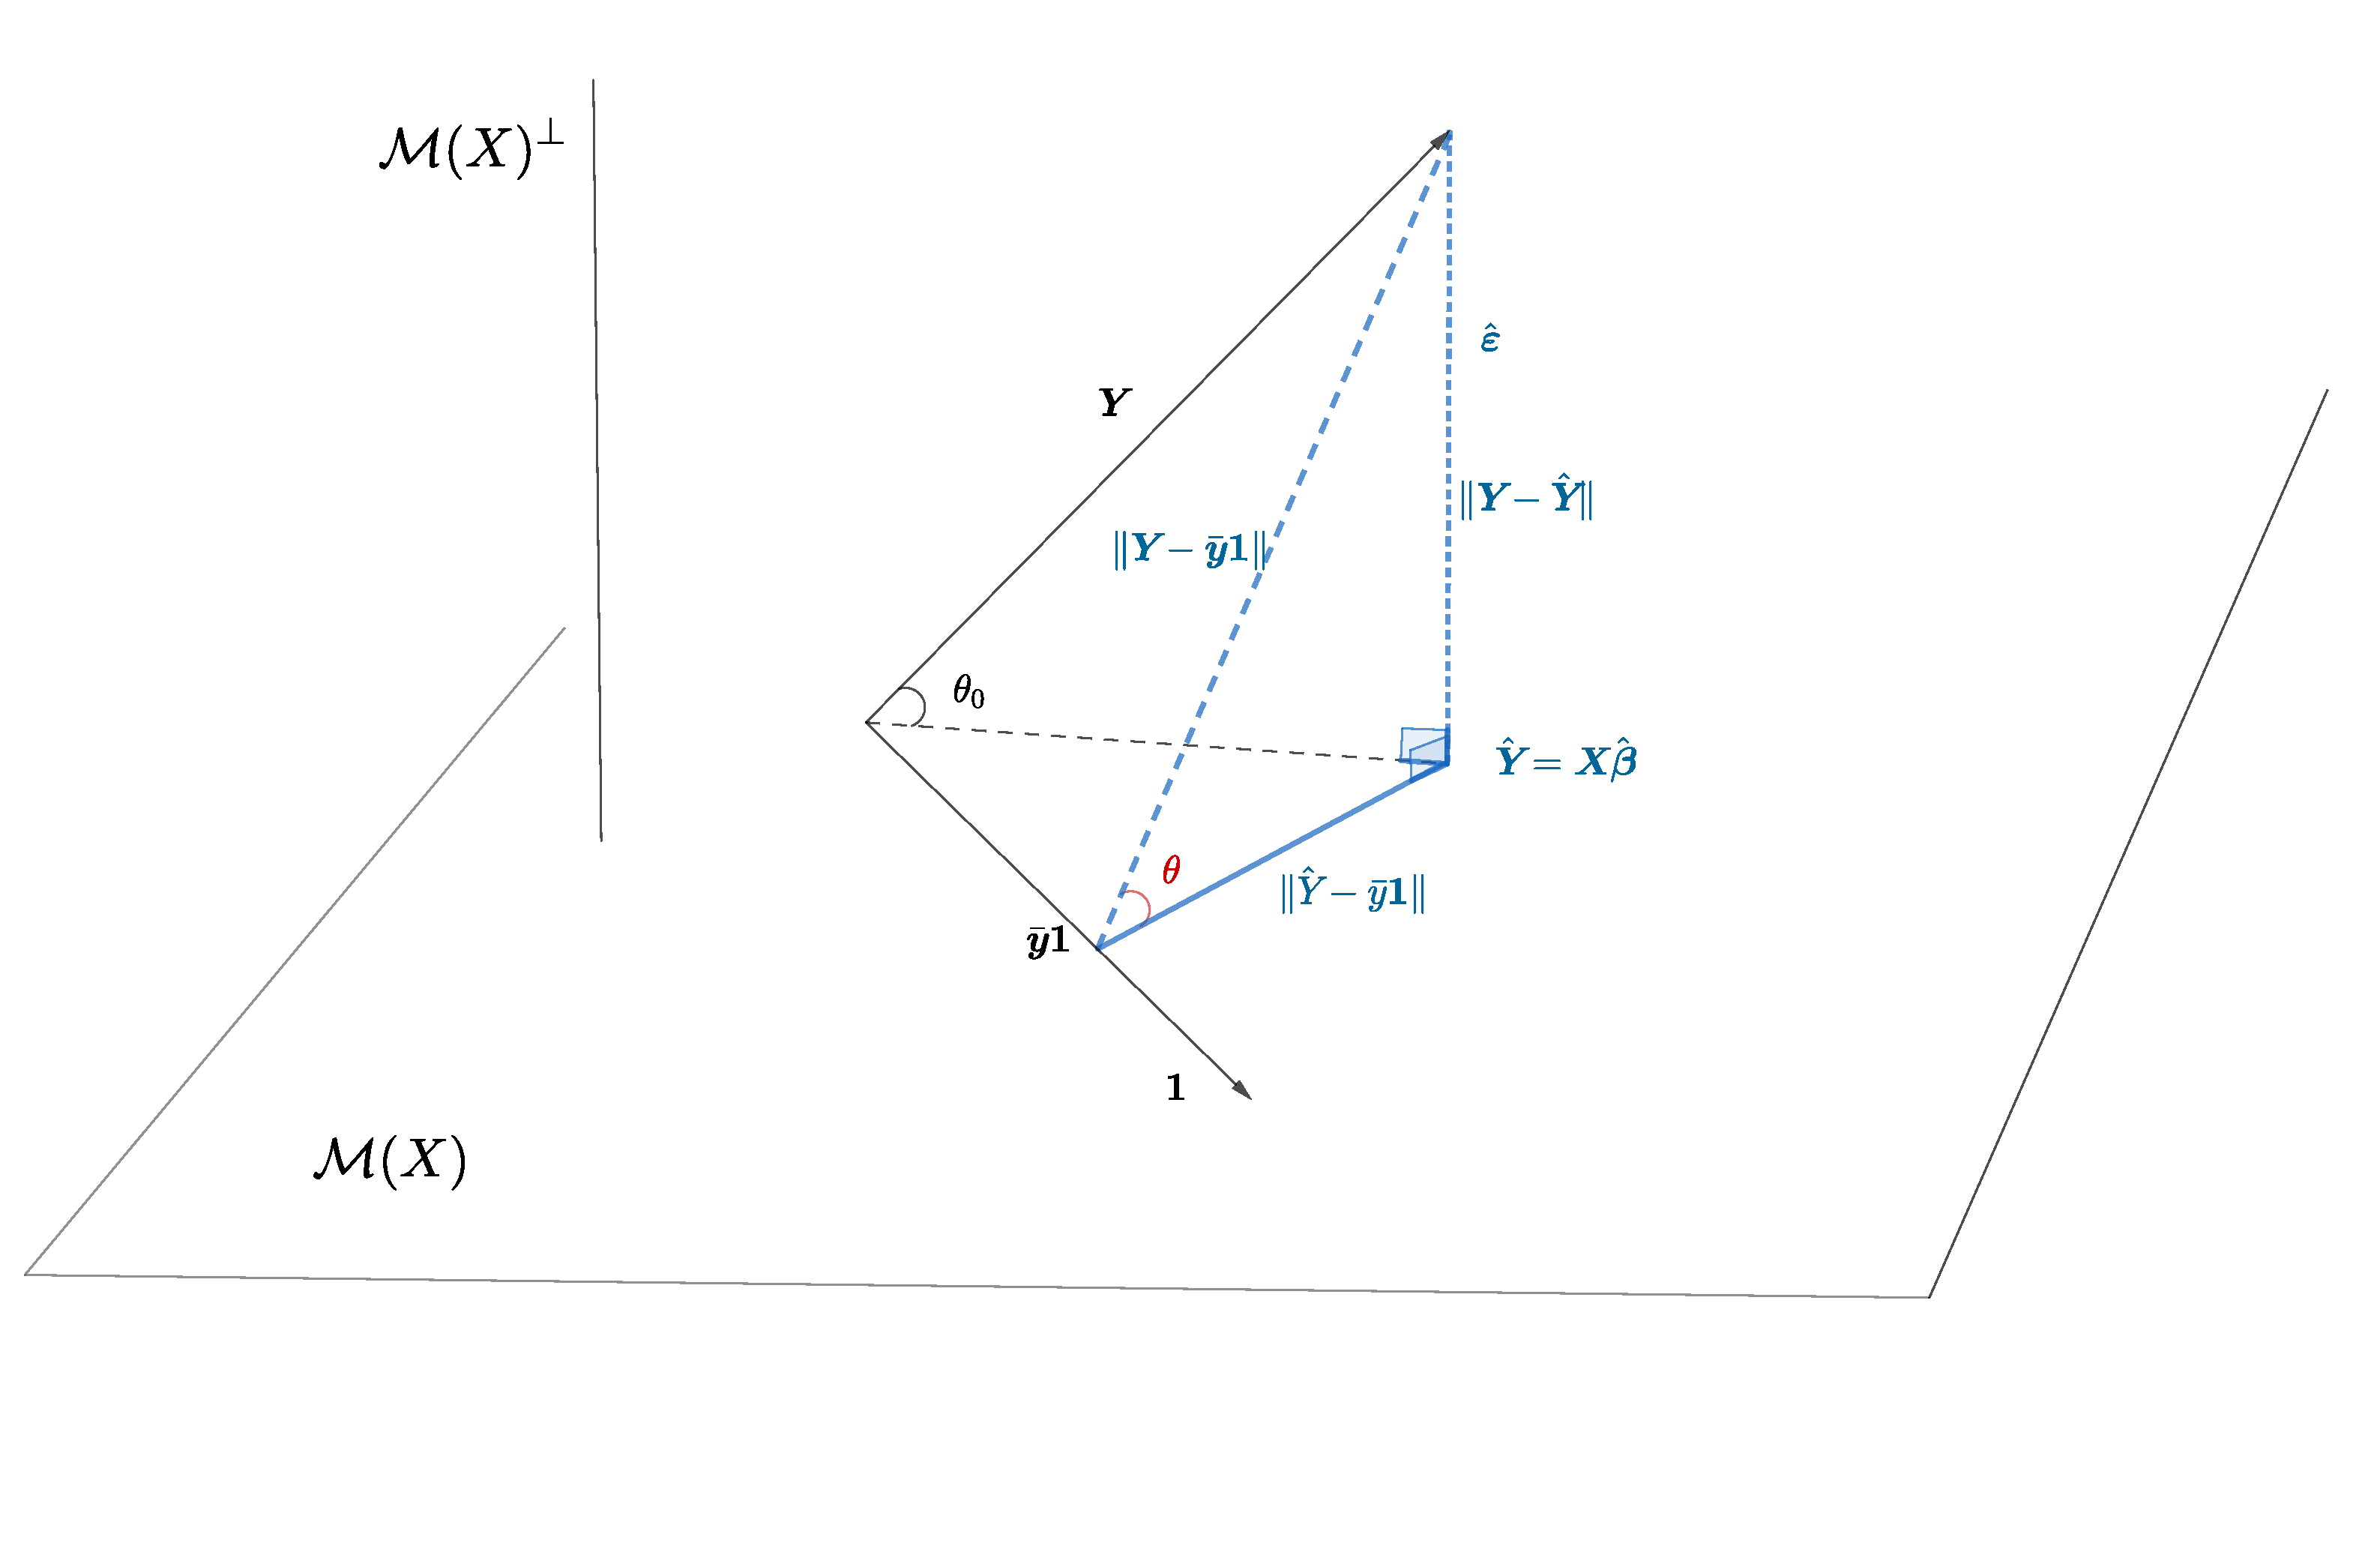
\includegraphics[width=0.7\linewidth]{images/sem2/RegMult_p2b} \end{center}

Conform figurii de mai sus observăm că putem aplica \emph{Teorema lui
Pitagora} în triunghiul albastru și obținem descompunerea

\[
  \lVert \boldsymbol Y - \bar{\boldsymbol y}\mathbf{1}\rVert^2 = \lVert \hat{\boldsymbol Y} - \bar{\boldsymbol y}\mathbf{1}\rVert^2 + \lVert\hat{\boldsymbol\varepsilon}\rVert^2
\]

unde

\begin{itemize}
\item
  \(SS_{T} = \lVert \boldsymbol Y - \bar{\boldsymbol y}\mathbf{1}\rVert^2\)
  se numește \textbf{suma abaterilor pătratice totale} (variația totală)
\item
  \(SS_{reg} = \lVert \hat{\boldsymbol Y} - \bar{\boldsymbol y}\mathbf{1}\rVert^2\)
  se numește \textbf{suma abaterilor pătratice de regresie} (variația
  explicată de model)
\item
  \(RSS = \lVert \boldsymbol Y - \hat{\boldsymbol Y}\rVert^2 = \lVert\hat{\boldsymbol\varepsilon}\rVert^2\)
  se numește \textbf{suma abaterilor pătratice reziduale} (variația
  reziduală)
\end{itemize}

\emph{Coeficientul de determinare} \(R^2\) (în \texttt{R} are denumirea
de \(\texttt{Multiple R-Squared}\)) este definit prin

\[
  R^2 = \cos^2(\theta) = \frac{\text{Variația explicată de model}}{\text{Variația totală}} = \frac{\lVert \hat{\boldsymbol Y} - \bar{\boldsymbol y}\mathbf{1}\rVert^2}{\lVert \boldsymbol Y - \bar{\boldsymbol y}\mathbf{1}\rVert^2} = 1 - \frac{\lVert\hat{\boldsymbol\varepsilon}\rVert^2}{\lVert \boldsymbol Y - \bar{\boldsymbol y}\mathbf{1}\rVert^2}
\] și ne dă proporția din variabilitatea lui \(\boldsymbol Y\) explicată
prin modelul de regresie. Cum \(R^2\) nu ține cont de dimensiunea
spațiului \(\mathcal{M}(X)\) se definește \emph{coeficientul de
determinare ajustat} \(R_a^2\) (în \texttt{R} are denumirea de
\(\texttt{Adjusted R-Squared}\)) prin

\[
  R_a^2 = 1 - \frac{\frac{\lVert\hat{\boldsymbol\varepsilon}\rVert^2}{n-(p+1)}}{\frac{\lVert \boldsymbol Y - \bar{\boldsymbol y}\mathbf{1}\rVert^2}{n-1}} = 1 - \frac{n-1}{n-(p+1)}\frac{\lVert\hat{\boldsymbol\varepsilon}\rVert^2}{\lVert \boldsymbol Y - \bar{\boldsymbol y}\mathbf{1}\rVert^2}.
\]

Ajustarea corespunde la împărțirea normelor la pătrat cu dimensiunea
subspațiului din care fac parte vectorii.

\begin{rmdexercise}
\marginnote{\enonce{23001}{}}\vspace{-7mm}

Ne propunem să determinăm evoluția unei variabile răspuns \(y_i\) în
funcție de două variabile explicative \(x_i\) și \(z_i\). Fie
\(\boldsymbol X = (\mathbf{1}, \boldsymbol x, \boldsymbol z)\) matricea
de design.

\begin{enumerate}
\def\labelenumi{\arabic{enumi}.}
\tightlist
\item
  Am obținut rezultatele următoare
\end{enumerate}

\[
  \boldsymbol X^\intercal\boldsymbol X = \begin{pmatrix}25 & 0 & 0\\
  ? & 9.3 & 5.4\\
  ? & ? & 12.7\end{pmatrix}
\]

\begin{enumerate}
\def\labelenumi{\alph{enumi})}
\item
  Determinați valorile care lipsesc (\texttt{?}).
\item
  Cât este \(n\) ?
\item
  Calculați coeficientul de corelație dintre \(\boldsymbol x\) și
  \(\boldsymbol z\).
\end{enumerate}

\begin{enumerate}
\def\labelenumi{\arabic{enumi}.}
\setcounter{enumi}{1}
\tightlist
\item
  Modelul de regresie liniară a lui \(\boldsymbol Y\) în funcție de
  \(\mathbf{1}, \boldsymbol x, \boldsymbol z\) este
\end{enumerate}

\[
  \boldsymbol Y = -1.6\boldsymbol 1 + 0.61 \boldsymbol x + 0.46 \boldsymbol z + \hat{\boldsymbol \varepsilon}, \quad \lVert\hat{\boldsymbol \varepsilon}\rVert^2 = 0.3
\]

\begin{enumerate}
\def\labelenumi{\alph{enumi})}
\item
  Determinați \(\bar{\boldsymbol y}\).
\item
  Calculați suma abaterilor pătratice de regresie \(SS_{reg}\), suma
  abaterilor pătratice totale \(SS_T\), coeficientul de determinare și
  coeficientul de determinare ajustat.
\end{enumerate}
\end{rmdexercise}

\begin{enumerate}
\def\labelenumi{\arabic{enumi}.}
\item
  \begin{enumerate}
  \def\labelenumii{\alph{enumii})}
  \tightlist
  \item
    Pentru a determina cele trei valori care lipsesc să notăm că
    matricea \(\boldsymbol X^\intercal\boldsymbol X\) este simetrică,
    prin urmare
    \(\boldsymbol X^\intercal\boldsymbol X = \left(\boldsymbol X^\intercal\boldsymbol X\right)^\intercal\)
    de unde
  \end{enumerate}
\end{enumerate}

\[
  \begin{pmatrix}25 & 0 & 0\\
  ? & 9.3 & 5.4\\
  ? & ? & 12.7\end{pmatrix} = \begin{pmatrix}25 & ? & ?\\
  0 & 9.3 & ?\\
  0 & 5.4 & 12.7\end{pmatrix}
\]

ceea ce conduce la valorile \(0, 0, 5.4\).

\begin{enumerate}
\def\labelenumi{\alph{enumi})}
\setcounter{enumi}{1}
\tightlist
\item
  Pentru a determina valoarea lui \(n\) să observăm că
\end{enumerate}

\[
  \boldsymbol X^\intercal\boldsymbol X = \begin{pmatrix}\mathbf{1}^\intercal \\
  \boldsymbol x^\intercal\\
  \boldsymbol z^\intercal\end{pmatrix}\begin{pmatrix}\mathbf{1} &
  \boldsymbol x &
  \boldsymbol z\end{pmatrix} = \begin{pmatrix}\mathbf{1}^\intercal \mathbf{1} & \mathbf{1}^\intercal\boldsymbol x & \mathbf{1}^\intercal\boldsymbol z \\
  \boldsymbol x^\intercal\mathbf{1} & \boldsymbol x^\intercal\boldsymbol x & \boldsymbol x^\intercal\boldsymbol z\\
  \boldsymbol z^\intercal\mathbf{1} & \boldsymbol z^\intercal\boldsymbol x & \boldsymbol z^\intercal\boldsymbol z\end{pmatrix} = \begin{pmatrix}n & n\bar x & n\bar z \\
  n\bar x & \boldsymbol x^\intercal\boldsymbol x & \boldsymbol x^\intercal\boldsymbol z\\
  n\bar z & \boldsymbol z^\intercal\boldsymbol x & \boldsymbol z^\intercal\boldsymbol z\end{pmatrix}
\]

ceea ce arată că
\(n = \left(\boldsymbol X^\intercal\boldsymbol X\right)_{1,1} = 25\).

\begin{enumerate}
\def\labelenumi{\alph{enumi})}
\setcounter{enumi}{2}
\tightlist
\item
  Coeficientul de corelație dintre \(\boldsymbol x\) și
  \(\boldsymbol z\) este dat de
\end{enumerate}

\[
  r_{\boldsymbol x,\boldsymbol z} = \frac{\sum_{i=1}^{n}(x_i - \bar x)(z_i - \bar z)}{\sqrt{\sum_{i = 1}^{n}(x_i - \bar x)^2}\sqrt{\sum_{i = 1}^{n}(z_i - \bar z)^2}}
\]

și cum, din punctul anterior,
\(\bar x = \frac{\left(\boldsymbol X^\intercal\boldsymbol X\right)_{1,2}}{n} = 0\)
și
\(\bar z = \frac{\left(\boldsymbol X^\intercal\boldsymbol X\right)_{1,3}}{n} = 0\)
deci

\[
  r_{\boldsymbol x,\boldsymbol z} = \frac{\sum_{i=1}^{n}x_iz_i}{\sqrt{\sum_{i = 1}^{n}x_i^2}\sqrt{\sum_{i = 1}^{n}z_i^2}} = \frac{\boldsymbol x^\intercal\boldsymbol z}{\sqrt{\boldsymbol x^\intercal\boldsymbol x}\sqrt{\boldsymbol z^\intercal\boldsymbol z}} = \frac{\left(\boldsymbol X^\intercal\boldsymbol X\right)_{2,3}}{\sqrt{\left(\boldsymbol X^\intercal\boldsymbol X\right)_{2,2}}\sqrt{\left(\boldsymbol X^\intercal\boldsymbol X\right)_{3,3}}} = \frac{5.4}{\sqrt{9.3}\sqrt{12.7}}\approx 0.5
\]

\begin{enumerate}
\def\labelenumi{\arabic{enumi}.}
\setcounter{enumi}{1}
\item
  \begin{enumerate}
  \def\labelenumii{\alph{enumii})}
  \tightlist
  \item
    Avem modelul
  \end{enumerate}
\end{enumerate}

\[
  y_i = -1.6 + 0.61 x_i + 0.46 z_i + \hat{\varepsilon}_i
\]

care prin sumare devine

\[
  \bar y = -1.6 + 0.61 \bar x + 0.46 \bar z + \frac{1}{n}\sum_{i=1}^{n}\hat{\varepsilon}_i.
\]

Cum \(\mathbf{1}\) aparține modelului, deci
\(\mathbf{1}\in\mathcal{M}(\boldsymbol X)\) și ținând cont de faptul că
\(\hat{\boldsymbol \varepsilon}\in\mathcal{M}(X)^\perp\) deducem că
\(\langle\mathbf{1}, \hat{\boldsymbol \varepsilon}\rangle = 0\) sau
\(\frac{1}{n}\sum_{i=1}^{n}\hat{\varepsilon}_i = 0\). Astfel

\[
  \bar y = -1.6 + 0.61 \underbrace{\bar x}_{=0} + 0.46 \underbrace{\bar z}_{= 0} + \underbrace{\frac{1}{n}\sum_{i=1}^{n}\hat{\varepsilon}_i}_{=0} = -1.6.
\]

\begin{enumerate}
\def\labelenumi{\alph{enumi})}
\setcounter{enumi}{1}
\tightlist
\item
  Avem că suma abaterilor pătratice explicate de model este dată de
\end{enumerate}

\[
  SS_{reg} = \lVert\hat{\boldsymbol Y} - \bar y\mathbf{1}\rVert^2 = \sum_{i=1}^{n}(\hat{y}_i - \bar y)^2 = \sum_{i=1}^{n}(0.61 x_i + 0.46 z_i)^2
\]

adică

\begin{align*}
  SS_{reg} &= \lVert\hat{\boldsymbol Y} - \bar y\mathbf{1}\rVert^2 = 0.61^2\sum_{i=1}^{n}x_i^2 + 2\times 0.61\times 0.46\sum_{i=1}^{n}x_iz_i + 0.46^2\sum_{i=1}^{n}z_i^2\\
  &= 0.61^2\left(\boldsymbol X^\intercal\boldsymbol X\right)_{2,2} + 2\times 0.61\times 0.46\left(\boldsymbol X^\intercal\boldsymbol X\right)_{2,3} + 0.46^2\left(\boldsymbol X^\intercal\boldsymbol X\right)_{3,3} = 9.18.
\end{align*}

Suma abaterilor pătratice totale se determină folosind formula de
descompunere a varianței:

\[
\underbrace{SS_T}_{\lVert\boldsymbol Y - \bar y\mathbf{1}\rVert^2} = \underbrace{SS_{reg}}_{\lVert\hat{\boldsymbol Y} - \bar y\mathbf{1}\rVert^2} + \underbrace{RSS}_{\lVert\hat{\boldsymbol \varepsilon}\rVert^2} = 9.18 + 0.3 = 9.48.
\]

Coeficientul de determinare \(R^2\) este

\[
  R^2 = \frac{SS_{reg}}{SS_T} = \frac{9.18}{9.48}\approx 0.968
\]

ceea ce arată că aproximativ \(97\%\) din variabilitatea datelor este
explicată de modelul de regresie iar coeficientul de determinare ajustat
este

\[
  R_1^2 = 1 - \frac{n-1}{n-(p+1)}\frac{\lVert\hat{\boldsymbol\varepsilon}\rVert^2}{\lVert \boldsymbol Y - \bar{\boldsymbol y}\mathbf{1}\rVert^2} = 1 - \frac{n-1}{n-(p+1)}\left(1 - R^2\right) = 1 - \frac{25 - 1}{25 - (2 + 1)}(1-0.968)\approx 0.965
\]

ceea ce verifică relația generală \(R_a^2<R^2\).

\begin{rmdexercise}
\marginnote{\enonce{23002}{}}\vspace{-7mm}

Fie \(\boldsymbol Z\in\mathcal{M}_{n,q}(\mathbb{R})\) o matrice de rang
\(q\) și \(\boldsymbol X\in\mathcal{M}_{n,p}(\mathbb{R})\) o matrice de
rang \(p\), \(p>q\), compusă din cei \(q\) vectori coloană ai lui
\(\boldsymbol Z\) și din alți \(p-q\) vectori liniar independenți.
Considerăm modelele următoare:

\begin{align*}
  \boldsymbol Y &= \boldsymbol Z\boldsymbol \beta + \boldsymbol\varepsilon,\\
  \boldsymbol Y &= \boldsymbol X\boldsymbol \gamma + \boldsymbol\eta
\end{align*}

Presupunem, pentru simplitate, că niciun model nu conține termenul liber
(constanta). Notăm cu \(P_X\) și \(P_Z\) matricele de proiecție
ortogonală pe subspațiile \(\mathcal{M}(X)\) și respectiv
\(\mathcal{M}(Z)\), generate de coloanele lui \(\boldsymbol X\) și
\(\boldsymbol Z\). De asemenea notăm cu \(P_{X\cap Z^\perp}\) matricea
de proiecție ortogonală pe \(\mathcal{M}(X)\cap \mathcal{M}(Z)^\perp\),
subspațiul ortogonal al lui \(\mathcal{M}(Z)\) din \(\mathcal{M}(X)\),
astfel

\[
  \mathbb{R}^n = \mathcal{M}(X) \oplus \mathcal{M}(X)^\perp = \left(\mathcal{M}(Z) \oplus \left(\mathcal{M}(X)\cap \mathcal{M}(Z)^\perp\right) \right) \oplus \mathcal{M}(X)^\perp
\]

\begin{enumerate}
\def\labelenumi{\arabic{enumi}.}
\item
  Exprimați \(\lVert P_X\boldsymbol Y\rVert^2\) în funcție de
  \(\lVert P_Z\boldsymbol Y\rVert^2\) și de
  \(\lVert P_{X\cap Z^\perp}\boldsymbol Y\rVert^2\).
\item
  Comparați coeficienții de determinare a celor două modele, \(R_Z^2\)
  și \(R_X^2\).
\end{enumerate}
\end{rmdexercise}

Acest exercițiu face referire la modele imbricate - \emph{nested
models}.

\begin{enumerate}
\def\labelenumi{\arabic{enumi}.}
\tightlist
\item
  Deoarece
  \(\mathcal{M}(\boldsymbol Z)\subset\mathcal{M}(\boldsymbol X)\) și
  aplicând \emph{teorema celor trei perpendiculare}\footnote{\emph{Teorema
    celor trei perpendiculare} spune că dacă \(\boldsymbol V\) și
    \(\boldsymbol W\) sunt două subspații vectoriale astfel încât
    \(\boldsymbol V\subset \boldsymbol W\) atunci
    \(P_V P_W = P_W P_V = P_V\).} avem, vezi figura de mai jos,
\end{enumerate}

\begin{align*}
  \hat{\boldsymbol Y}_p &= P_X\boldsymbol Y = (\underbrace{P_Z + P_{Z^\perp}}_{I}) P_X\boldsymbol Y = P_Z P_X \boldsymbol Y + P_{Z^\perp}P_X\boldsymbol Y\\
  &= P_X\boldsymbol Y + P_{X\cap Z^\perp} \boldsymbol Y = \hat{\boldsymbol Y}_q + P_{X\cap Z^\perp} \boldsymbol Y
\end{align*}

și din Teorema lui Pitagora (vezi triunghiul roșu) deducem că

\[
  \lVert P_X\boldsymbol Y\rVert^2 = \lVert P_Z\boldsymbol Y\rVert^2 + \lVert P_{X\cap Z^\perp}\boldsymbol Y\rVert^2.
\]

\begin{center}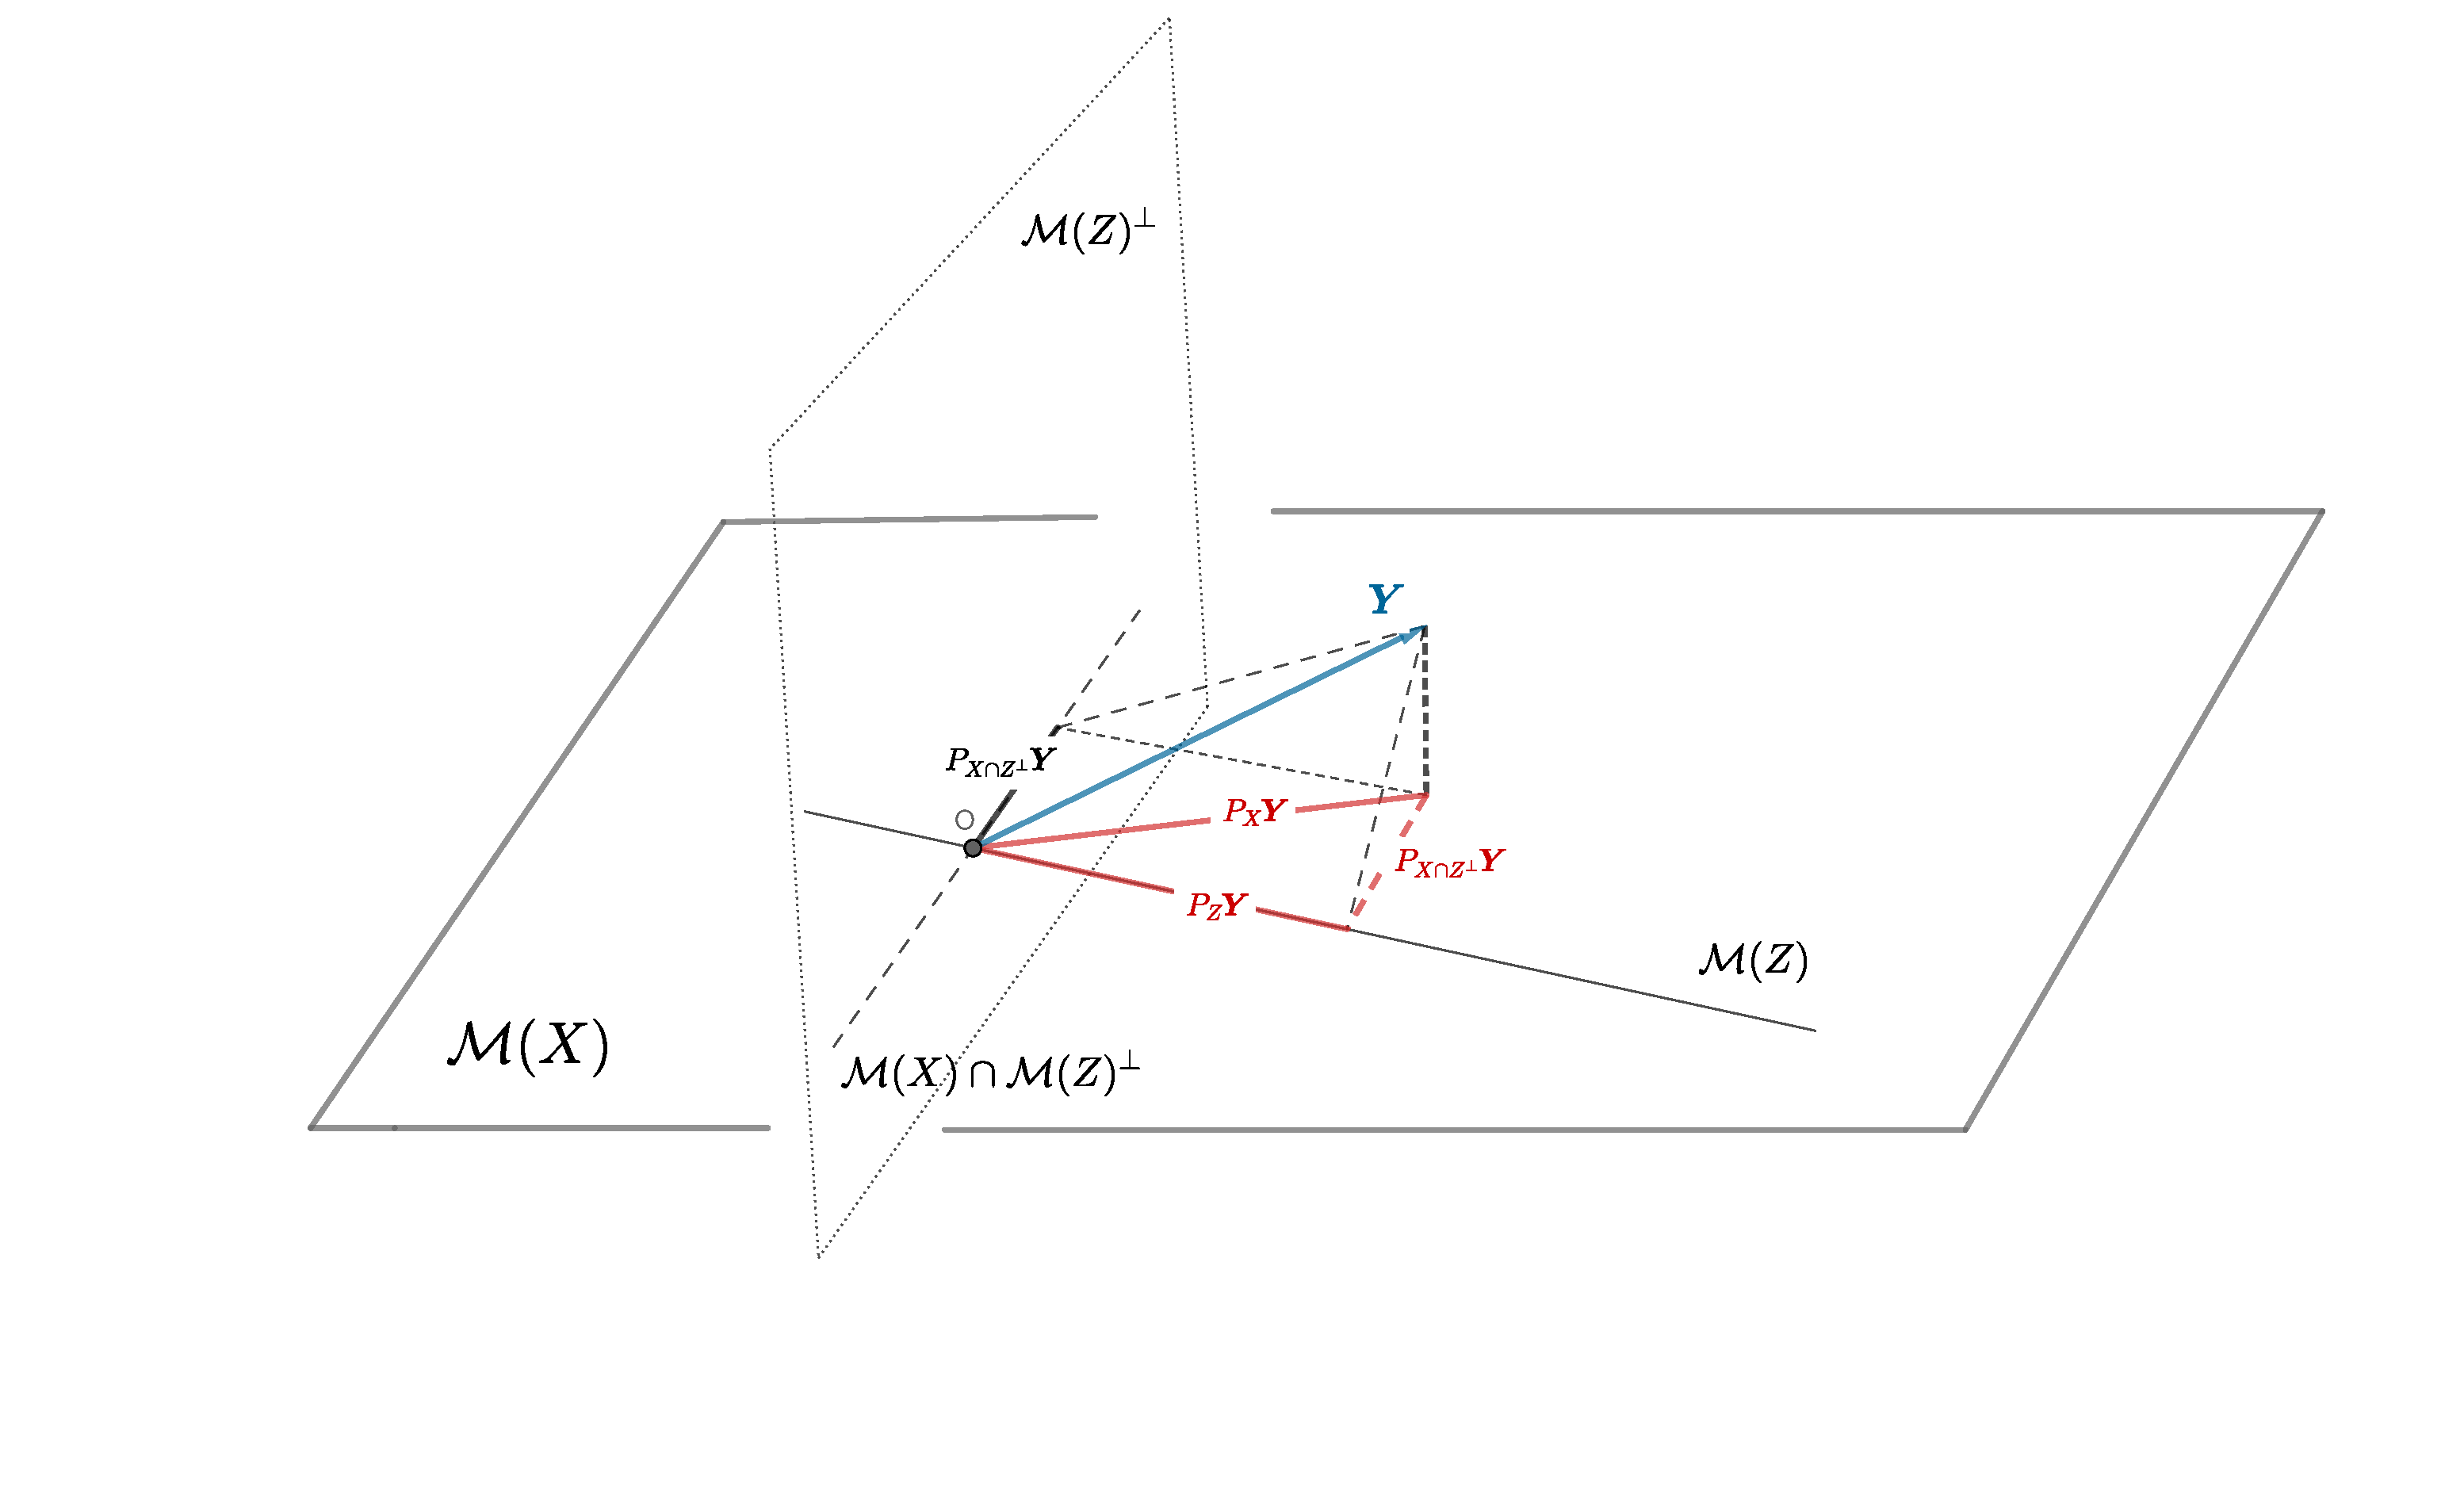
\includegraphics[width=0.7\linewidth]{images/sem2/RegMult_p2c} \end{center}

\begin{enumerate}
\def\labelenumi{\arabic{enumi}.}
\setcounter{enumi}{1}
\tightlist
\item
  Dacă modelul nu are termenul liber (constanta) atunci coeficientul de
  determinare este definit prin
  \(R_X^2 = \frac{\lVert P_{X}\boldsymbol Y\rVert^2}{\lVert\boldsymbol Y\rVert^2}\)
  prin urmare
\end{enumerate}

\[
  R_X^2 = \frac{\lVert P_{X}\boldsymbol Y\rVert^2}{\lVert\boldsymbol Y\rVert^2} = \frac{\lVert P_Z\boldsymbol Y\rVert^2 + \lVert P_{X\cap Z^\perp}\boldsymbol Y\rVert^2}{\lVert\boldsymbol Y\rVert^2} = R_Z^2 + \frac{\lVert P_{X\cap Z^\perp}\boldsymbol Y\rVert^2}{\lVert\boldsymbol Y\rVert^2}\geq R_Z^2.
\]

Rezultatul de mai sus se generalizează și în cazul modelelor imbricate
care conțin termenul constant și ne spune arată că modelul mai mare are
un coeficient de determinare superior modelului mai mic. Altfel spus,
dacă la un model dat adăugăm una sau mai multe variabile explicative
ameliorăm variabilitatea explicată de model, chiar dacă variabilele
explicative suplimentare nu sunt pertinente! În acest caz este de
preferat coeficientul de determinare ajustat.

\begin{rmdexercise}
\marginnote{\enonce{23003}{}}\vspace{-7mm}

Considerăm modelul de regresie liniară

\[
  \boldsymbol Y = \boldsymbol X\boldsymbol \beta + \boldsymbol\varepsilon
\]

unde \(\boldsymbol Y\in\mathbb{R}^n\),
\(\boldsymbol X \in\mathcal{M}_{n, p}(\mathbb{R})\) este o matrice
compusă din \(p\) vectori ortogonali,
\(\boldsymbol \beta\in\mathbb{R}^{p}\) iar
\(\boldsymbol \varepsilon\in\mathbb{R}^n\). Fie \(\boldsymbol Z\)
matricea formată din primele \(q\) coloane ale lui \(\boldsymbol X\) și
\(\boldsymbol U\) matricea formată din ultimele \(p-q\) coloane ale lui
\(\boldsymbol X\). Prin metoda celor mai mici pătrate obținem

\begin{align*}
  \hat{\boldsymbol Y}_X &= \hat{\beta}_1^X \boldsymbol X_1 + \cdots + \hat{\beta}_p^X \boldsymbol X_p\\
  \hat{\boldsymbol Y}_Z &= \hat{\beta}_1^Z \boldsymbol X_1 + \cdots + \hat{\beta}_q^Z \boldsymbol X_q\\
  \hat{\boldsymbol Y}_U &= \hat{\beta}_{q+1}^U \boldsymbol X_{q+1} + \cdots + \hat{\beta}_p^U \boldsymbol X_p
\end{align*}

\begin{enumerate}
\def\labelenumi{\arabic{enumi}.}
\tightlist
\item
  Arătați că
  \(\lVert P_X\boldsymbol Y\rVert^2 = \lVert P_Z\boldsymbol Y\rVert^2 + \lVert P_U\boldsymbol Y\rVert^2\).
\item
  Pentru \(i\in\{1,2,\ldots,p\}\) dat, arătați că
  \(\hat{\beta}_i^X = \hat{\beta}_i^Z\) dacă \(i\leq q\) și
  \(\hat{\beta}_i^X = \hat{\beta}_i^U\) altfel.
\end{enumerate}
\end{rmdexercise}

\begin{enumerate}
\def\labelenumi{\arabic{enumi}.}
\tightlist
\item
  Cum \(P_Z + P_{Z^\perp} = I\) putem scrie
\end{enumerate}

\[
  \hat{\boldsymbol Y}_X = P_X\boldsymbol Y = (P_Z + P_{Z^\perp})P_X\boldsymbol Y = P_ZP_X\boldsymbol Y + P_{Z^\perp}P_X\boldsymbol Y,
\]

și din \(P_ZP_X = P_{Z\cap X} = P_Z\) găsim că
\(\hat{\boldsymbol Y}_X = P_Z\boldsymbol Y + P_{Z^\perp}P_X\boldsymbol Y\).
De asemenea, să notăm că \(P_{Z^\perp}P_X = P_{Z^\perp\cap X}\) și
ținând cont de faptul că matricea \(\boldsymbol X\) are coloanele
ortogonale avem \(P_{Z^\perp\cap X} = P_U\) (în fapt ortogonalitatea
coloanelor lui \(\boldsymbol X\) implică
\(\mathcal{M}(X) = \mathcal{M}(Z)\overset{\perp}{\oplus}\mathcal{M}(U)\),
sumă directă de spații ortogonale). Prin urmare obținem descompunerea
ortogonală

\[
  \hat{\boldsymbol Y}_X = P_Z\boldsymbol Y + P_U\boldsymbol Y = \hat{\boldsymbol Y}_Z + \hat{\boldsymbol Y}_U
\]

și din Teorema lui Pitagora avem

\[
  \lVert P_X\boldsymbol Y\rVert^2 = \lVert P_Z\boldsymbol Y\rVert^2 + \lVert P_U\boldsymbol Y\rVert^2. 
\]

\begin{enumerate}
\def\labelenumi{\arabic{enumi}.}
\setcounter{enumi}{1}
\tightlist
\item
  Vom arăta relația pentru \(i\leq q\), cazul general fiind analog. Din
  formula generală avem că \(\hat{\boldsymbol\beta}^X\) este
\end{enumerate}

\[
  \hat{\boldsymbol\beta}^X = \left(\boldsymbol X^\intercal \boldsymbol X\right)^{-1}\boldsymbol X^\intercal\boldsymbol Y
\]

și cum coloanele lui \(\boldsymbol X\) sunt ortogonale deducem că
matricea \(\boldsymbol X^\intercal\boldsymbol X\) este o matrice
diagonală,
\(\boldsymbol X^\intercal\boldsymbol X = \mathrm{diag}\left(\lVert\boldsymbol X_1\rVert^2, \ldots, \lVert\boldsymbol X_p\rVert^2\right)\).
Notând de asemenea că \(\boldsymbol X^\intercal\boldsymbol Y\) este un
vector coloană cu elemente de tipul
\(\langle\boldsymbol X_i, \boldsymbol Y\rangle\), deducem că

\[
  \hat{\boldsymbol\beta}^X = \begin{pmatrix}\frac{\langle\boldsymbol X_1, \boldsymbol Y\rangle}{\lVert\boldsymbol X_1\rVert^2} & \cdots & \frac{\langle\boldsymbol X_p, \boldsymbol Y\rangle}{\lVert\boldsymbol X_p\rVert^2}\end{pmatrix}^\intercal,
\] prin urmare
\(\hat{\boldsymbol\beta}_i^X = \frac{\langle\boldsymbol X_i, \boldsymbol Y\rangle}{\lVert\boldsymbol X_i\rVert^2}\).
Pentru \(i\leq q\), coloana \(i\) a matricei \(\boldsymbol Z\) este
\(\boldsymbol Z_i = \boldsymbol X_i\) și aplicând raționamentul anterior
găsim că

\[
\hat{\boldsymbol\beta}_i^Z = \frac{\langle\boldsymbol Z_i, \boldsymbol Y\rangle}{\lVert\boldsymbol Z_i\rVert^2} = \frac{\langle\boldsymbol X_i, \boldsymbol Y\rangle}{\lVert\boldsymbol X_i\rVert^2} = \hat{\boldsymbol\beta}_i^X.
\]

Rezultatul exercițiului ne spune că în cazul în care variabilele
explicative sunt ortogonale, a efectua o regresie multiplă revine la a
efectua \(p\) regresii simple.

\subsection{Modelul (condiționat)
normal}\label{modelul-conditionat-normal}

Considerăm modelul de regresie
\(\boldsymbol Y = \boldsymbol X\boldsymbol \beta + \boldsymbol \varepsilon\)
în care \(\boldsymbol Y\in\mathbb{R}^n\) este vectorul răspuns,
\(\boldsymbol X = \left[\mathbf{1}|\boldsymbol X_1|\cdots|\boldsymbol X_p\right]\in\mathcal{M}_{n, p+1}(\mathbb{R})\)
este matricea de design, \(\boldsymbol \beta\in\mathbb{R}^{p+1}\) este
vectorul parametrilor și \(\boldsymbol \varepsilon\in\mathbb{R}^n\) este
vectorul erorilor. Până acum, ipotezele modelului erau

\[
  \begin{array}{ll}
    \mathcal{H}_1: \, rang(\boldsymbol X) = p+1\\
    \mathcal{H}_2: \, \mathbb{E}[\boldsymbol \varepsilon] = 0,\, Var(\boldsymbol \varepsilon) = \sigma^2 I_n
  \end{array}
\]

În această secțiune ne propunem să studiem proprietățile statistice ale
modelului de regresie liniară plasându-ne într-un context parametric și
anume în contextul modelului gaussian:

\[
  \begin{array}{ll}
    \mathcal{H}_1: \, rang(\boldsymbol X) = p+1\\
    \mathcal{H}_2': \, \boldsymbol \varepsilon \sim\mathcal{N}(0, \sigma^2 I_n)
  \end{array}
\]

Observăm că ipoteza \(\mathcal{H}_2'\) este un caz particular al
ipotezei \(\mathcal{H}_2\) și în plus implică faptul că reziduurile sunt
independente și identic repartizate. Ipoteza de normalitate a erorilor
ne permite să scriem funcția de verosimilitate, să deducem repartițiile
estimatorilor propuși, să construim intervale de încredere și să testăm
ipoteze statistice.

\begin{rmdexercise}
\marginnote{\enonce{24001}{}}\vspace{-7mm}

Considerăm modelul de regresie liniară

\[
  \boldsymbol Y = \boldsymbol X\boldsymbol \beta + \boldsymbol\varepsilon
\]

sub ipotezele \(\mathcal{H}_1\) și \(\mathcal{H}_2'\) de mai sus.
Determinați estimatorii de verosimilitate maximă pentru
\(\boldsymbol \beta\) și \(\boldsymbol\varepsilon\).
\end{rmdexercise}

Începem prin a observa că din modelul de regresie

\[
  y_i = \boldsymbol x_i^\intercal\boldsymbol\beta + \varepsilon_i
\]

și conform ipotezei \(\mathcal{H}_2'\) avem
\(\varepsilon_i\sim\mathcal{N}(0, \sigma^2)\) prin urmare
\(y_i\sim\mathcal{N}(\boldsymbol x_i^\intercal\boldsymbol\beta, \sigma^2)\)
și în plus \(y_i\) sunt variabile aleatoare independete deoarece
\(\varepsilon_i\) sunt independente. Astfel funcția de verosimilitate se
scrie

\begin{align*}
  L(\boldsymbol\beta, \sigma^2;\boldsymbol Y) &= \prod_{i = 1}^{n}f_{Y}(y_i) = \left(\frac{1}{\sqrt{2\pi\sigma^2}}\right)^n e^{-\frac{1}{2\sigma^2}\sum_{i = 1}^{n}(y_i - \boldsymbol x_i^\intercal\boldsymbol\beta)^2} \\
  &= \left(\frac{1}{\sqrt{2\pi\sigma^2}}\right)^n e^{-\frac{1}{2\sigma^2}\lVert\boldsymbol Y - \boldsymbol X\boldsymbol\beta\rVert^2}
\end{align*}

ceea ce conduce la logaritmul funcției de verosimilitate

\[
  l(\boldsymbol\beta, \sigma^2;\boldsymbol Y) = \log  L(\boldsymbol\beta, \sigma^2;\boldsymbol Y) = -\frac{n}{2}\log{2\pi\sigma^2} -\frac{1}{2\sigma^2}\lVert\boldsymbol Y - \boldsymbol X\boldsymbol\beta\rVert^2.
\]

Vrem să determinăm

\[
  (\hat{\boldsymbol\beta}_{VM}, \hat{\sigma}_{VM}^2) = \underset{(\boldsymbol\beta, \sigma^2)\in\mathbb{R}^{p+1}\times(0,\infty)}{\arg\max} l(\boldsymbol\beta, \sigma^2;\boldsymbol Y)
\]

și observăm că pentru \(\sigma^2\) fixat, a maximiza funcția
\(l(\boldsymbol\beta, \sigma^2;\boldsymbol Y)\) revine la a determina
valoarea lui \(\boldsymbol\beta\) care minimizează
\(\lVert\boldsymbol Y - \boldsymbol X\boldsymbol\beta\rVert^2\), aceasta
ne fiind alta decât \(\hat{\boldsymbol\beta}\) obținut prin metoda celor
mai mici pătrate. Astfel găsim că

\[
  \hat{\boldsymbol\beta}_{VM} = \hat{\boldsymbol\beta} = (\boldsymbol{X}^\intercal \boldsymbol X)^{-1}\boldsymbol{X}^\intercal \boldsymbol Y.
\]

Pentru a determina \(\hat{\sigma}_{VM}^2\) să observăm că problema
revine la a determina soluția ecuației

\[
  \frac{\partial l(\hat{\boldsymbol\beta}_{VM}, \sigma^2;\boldsymbol Y)}{\partial \sigma^2} = -\frac{n}{2\sigma^2} + \frac{1}{2\sigma^4}\lVert\boldsymbol Y - \boldsymbol X\hat{\boldsymbol\beta}_{VM}\rVert^2 = 0
\]

care este
\(\hat{\sigma}_{VM}^2 = \frac{\lVert\boldsymbol Y - \boldsymbol X\hat{\boldsymbol\beta}_{VM}\rVert^2}{n}=\frac{\lVert\boldsymbol Y - \boldsymbol X\hat{\boldsymbol\beta}\rVert^2}{n}\).
Comparând acest rezultat cu cel obținut prin metoda celor mai mici
pătrate observăm că

\[
  \hat{\sigma}_{VM}^2 = \frac{n - (p+1)}{n}\hat{\sigma}^2, 
\]

deci estimatorul de verosimilitate maximă \(\hat{\sigma}_{VM}^2\) a lui
\(\sigma^2\) est un estimator deplasat. În cele ce urmează vom considera
estimatorul nedeplasat
\(\hat{\sigma}^2 = \frac{\lVert\boldsymbol Y - \boldsymbol X\hat{\boldsymbol\beta}\rVert^2}{n - (p+1)} = \frac{\sum_{i=1}^{n}\hat{\varepsilon}_i}{n - (p+1)}\)
ca estimator al lui \(\sigma^2\).

\subsubsection{Repartițiile estimatorilor, intervale și regiuni de
încredere}\label{repartitiile-estimatorilor-intervale-si-regiuni-de-incredere}

Înainte de a investiga repartițiile estimatorilor
\(\hat{\boldsymbol\beta}\) și \(\hat{\sigma}^2\) pentru modelul de
regresie liniară sub ipoteza de normalitate, să reamintim câteva noțiuni
legate de vectorii gaussieni (pentru mai multe detalii se poate consulta
\citep[Capitolul 2]{Seber2003} sau \citep[Capitolul 16]{Jacod2003}).

Spunem că un vector \(\boldsymbol Y = (Y_1,\ldots,Y_n)\in\mathbb{R}^n\)
este un vector gaussian dacă toate combinațiile liniare
\(\sum_{i=1}^{n}a_iY_i\) sunt repartizate normal (posibil degenerat dacă
toți coeficienții sunt nuli). Acest vector admite o medie
\(\boldsymbol\mu = \mathbb{E}[\boldsymbol Y]\) și o matrice de
varianță-covarianță
\(\Sigma_{\boldsymbol Y} = \mathbb{E}[(\boldsymbol Y - \boldsymbol\mu)(\boldsymbol Y - \boldsymbol\mu)^\intercal]\)
care caracterizează complet repartiția lui \(\boldsymbol Y\). În acest
caz notăm
\(\boldsymbol Y \sim\mathcal{N}(\boldsymbol\mu, \Sigma_{\boldsymbol Y})\).
Un vector gaussian \(\boldsymbol Y\) admite o densitate de repartiție
\(f_{\boldsymbol Y}\) pe \(\mathbb{R}^n\) dacă și numai dacă matricea sa
de varianță-covarianță \(\Sigma_{\boldsymbol Y}\) este inversabilă și în
acest caz

\[
  f_{\boldsymbol Y}(\boldsymbol y) = \frac{1}{(2\pi)^{\frac{n}{2}}\sqrt{\det{\Sigma_{\boldsymbol Y}}}} e^{-\frac{1}{2}(\boldsymbol y - \boldsymbol \mu)^\intercal \Sigma_{\boldsymbol Y}^{-1}(\boldsymbol y - \boldsymbol \mu)}
\]

În cazul în care matricea \(\Sigma_{\boldsymbol Y}\) nu este inversabilă
înseamnă că \(\boldsymbol Y\) ia valori într-un subspațiu de dimensiune
\(n_0<n\) unde este repartizat ca un vector gaussian de dimensiune
\(n_0\).

Figura de mai jos prezintă patru repartiții normale bivariate (\(n=2\))
\(\boldsymbol Y \sim\mathcal{N}(\boldsymbol\mu, \Sigma_{\boldsymbol Y})\),
cu \(\boldsymbol\mu = (\mu_1, \mu_2)^\intercal\) iar
\(\Sigma_{\boldsymbol Y} = \begin{pmatrix}\sigma_{11} & \sigma_{12}\\ \sigma_{21} & \sigma_{22}\end{pmatrix}= \begin{pmatrix}\sigma_{1}^2 & \sigma_{12}\\ \sigma_{12} & \sigma_{2}^2\end{pmatrix}\),
rotite cu unghiul \(\alpha\). În acest caz densitatea de repartiție este

\[
f_{\boldsymbol Y}(y_1,y_2) = \frac{1}{2\pi\sigma_1\sigma_2\sqrt{1-\rho^2}}e^{-\frac{1}{2(1-\rho^2)}\left[\left(\frac{y_1 - \mu_1}{\sigma_1}\right)^2 - 2\rho\left(\frac{y_1 - \mu_1}{\sigma_1}\right)\left(\frac{y_2 - \mu_2}{\sigma_2}\right) + \left(\frac{y_2 - \mu_2}{\sigma_2}\right)^2\right]}
\]

unde \(\rho = \frac{\sigma_{12}}{\sigma_1\sigma_2}\) este coeficientul
de corelație.

\begin{center}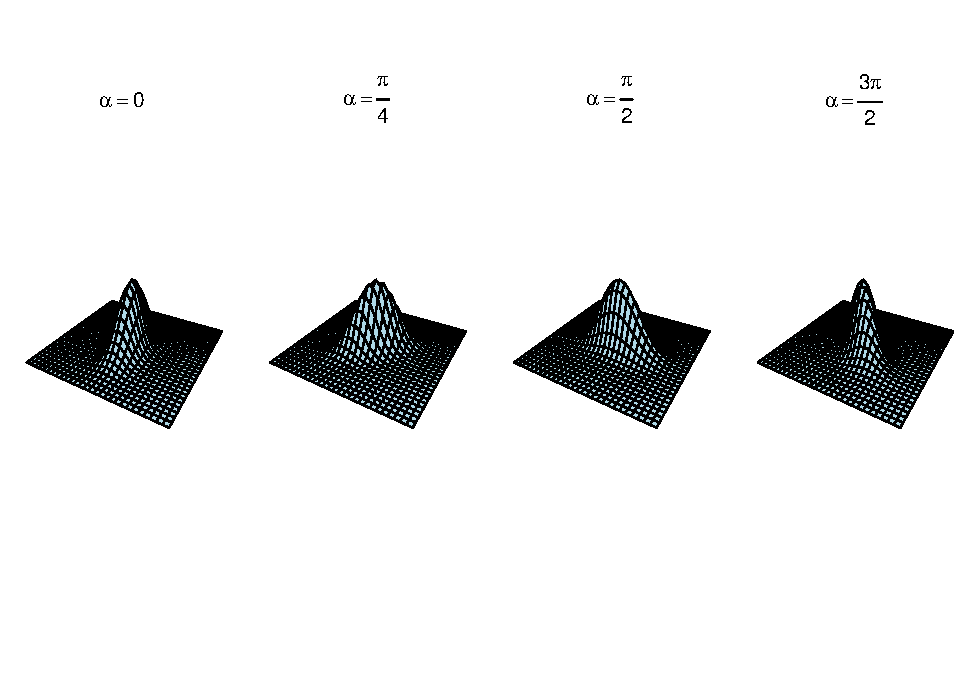
\includegraphics[width=0.85\linewidth]{Sem_2_files/figure-latex/unnamed-chunk-29-1} \end{center}

Una dintre proprietățile importante ale vectorilor gaussieni este
stabilitatea prin transformări afine: dacă
\(\boldsymbol A\in\mathcal{M}_{m,n}(\mathbb{R})\) și
\(\boldsymbol b\in\mathcal{M}_{m,1}(\mathbb{R})\) sunt respectiv o
matrice și un vector de scalari atunci

\[
  \boldsymbol Y \sim\mathcal{N}(\boldsymbol\mu, \Sigma_{\boldsymbol Y}) \Longrightarrow \boldsymbol A\boldsymbol Y + \boldsymbol b \sim\mathcal{N}(\boldsymbol A\boldsymbol\mu + \boldsymbol b, \boldsymbol A\Sigma_{\boldsymbol Y}\boldsymbol A^\intercal)
\]

De asemenea, plecând de la funcția caracteristică, se poate verifica
proprietatea de independență a componentelor unui vector gaussian care
ne spune că acestea sunt independente dacă și numai dacă matricea de
varianță-covarianță este o matrice diagonală.

Avem următorul rezultat care face legătura dintre repartiția normală și
repartiția \(\chi^2\):

\begin{rmdinsight}
Fie
\(\boldsymbol Y \sim\mathcal{N}(\boldsymbol\mu, \Sigma_{\boldsymbol Y})\)
un vector gaussian în \(\mathbb{R}^n\). Dacă \(\Sigma_{\boldsymbol Y}\)
este o matrice inversabilă atunci

\[
  (\boldsymbol Y - \boldsymbol \mu)^\intercal \Sigma_{\boldsymbol Y}^{-1}(\boldsymbol Y - \boldsymbol \mu) \sim \chi_n^2
\]

repartiția \(\chi^2\) cu \(n\) grade de libertate.
\end{rmdinsight}

Deoarece matricea de varianță-covarianță \(\Sigma_{\boldsymbol Y}\) este
o matrice simetrică și pozitiv definită atunci din
\href{https://en.wikipedia.org/wiki/Eigendecomposition_of_a_matrix}{Teorema
de descompunere spectrală} ea se poate descompune sub forma
\(\Sigma_{\boldsymbol Y} = \boldsymbol Q\boldsymbol\Delta \boldsymbol Q^\intercal\)
unde \(\boldsymbol Q = [\boldsymbol v_1,\ldots,\boldsymbol v_n]\) este o
matrice ortogonală (\(\boldsymbol Q^\intercal = \boldsymbol Q^{-1}\))
formată din vectorii proprii \(\boldsymbol v_1,\ldots,\boldsymbol v_n\)
corespunzători valorilor proprii \(\lambda_1,\ldots,\lambda_n\), iar
\(\boldsymbol \Delta\) este matricea diagonală
\(\mathrm{diag}(\lambda_1,\ldots,\lambda_n)\). Dacă notăm cu
\(\boldsymbol \Delta^{-\frac{1}{2}}\) matricea diagonală de coeficienți
diagonali
\(\frac{1}{\sqrt{\lambda_1}},\ldots,\frac{1}{\sqrt{\lambda_n}}\) (aceste
fracții există deoarece pozitiv definirea matricei
\(\Sigma_{\boldsymbol Y}\) implică faptul că valorile proprii
\(\lambda_i>0\), \(i = 1,\ldots,n\)) atunci

\[
\Sigma_{\boldsymbol Y} = \boldsymbol Q\boldsymbol\Delta \boldsymbol Q^\intercal \Longrightarrow \Sigma_{\boldsymbol Y}^{-1} = \boldsymbol Q\boldsymbol\Delta^{-1} \boldsymbol Q^\intercal = \left(\boldsymbol Q\boldsymbol\Delta^{-\frac{1}{2}} \boldsymbol Q^\intercal\right)\left(\boldsymbol Q\boldsymbol\Delta^{-\frac{1}{2}} \boldsymbol Q^\intercal\right) = \Sigma_{\boldsymbol Y}^{-\frac{1}{2}}\Sigma_{\boldsymbol Y}^{-\frac{1}{2}}.
\]

Prin urmare găsim că

\[
(\boldsymbol Y - \boldsymbol \mu)^\intercal \Sigma_{\boldsymbol Y}^{-1}(\boldsymbol Y - \boldsymbol \mu) = \left(\Sigma_{\boldsymbol Y}^{-\frac{1}{2}}(\boldsymbol Y - \boldsymbol \mu)\right)^\intercal\left(\Sigma_{\boldsymbol Y}^{-\frac{1}{2}}(\boldsymbol Y - \boldsymbol \mu)\right) 
\]

și cum vectorii gaussieni rămân gaussieni și prin aplicarea unor
transformări afine (vezi rezultatul de mai sus) avem că

\[
\boldsymbol Y \sim\mathcal{N}(\boldsymbol\mu, \Sigma_{\boldsymbol Y}) \Longrightarrow \Sigma_{\boldsymbol Y}^{-\frac{1}{2}}(\boldsymbol Y - \boldsymbol \mu) \sim\mathcal{N}(0, I_n).
\]

Astfel vectorul
\(\boldsymbol V = [\boldsymbol V_1,\ldots,\boldsymbol V_n]^\intercal = \Sigma_{\boldsymbol Y}^{-\frac{1}{2}}(\boldsymbol Y - \boldsymbol \mu)\),
care nu este altceva decât vectorul \(\boldsymbol Y\) centrat și redus,
este gaussian standard (\(\boldsymbol V_j\sim\mathcal{N}(0,1)\) și
\(\boldsymbol V_i\) și \(\boldsymbol V_j\) sunt independente) și

\[
(\boldsymbol Y - \boldsymbol \mu)^\intercal \Sigma_{\boldsymbol Y}^{-1}(\boldsymbol Y - \boldsymbol \mu) = \lVert \boldsymbol V\rVert^2 = \boldsymbol V_1^2 + \cdots + \boldsymbol V_n^2\sim\chi^2_n.
\]

Următorul rezultat, cunoscut sub denumirea de
\href{https://en.wikipedia.org/wiki/Cochran\%27s_theorem}{Teorema lui
Cochran}, asigură că descompunerea unui vector gaussian în componente
independente pe subspații ortogonale ne dă vectori independenți a căror
repartiție o putem explicita. Această teoremă poate fi văzută și ca o
generalizare a Teoremei lui Pitagora:

\begin{rmdinsight}
Fie \(\boldsymbol Y \sim\mathcal{N}(\boldsymbol\mu, \sigma^2 I_n)\),
\(\mathcal{M}\subset\mathbb{R}^n\) un subspațiu de dimensiune \(p\),
\(P\) matricea de proiecție ortogonală pe \(\mathcal{M}\) și
\(P_\perp = I_n - P\) matricea de proiecție ortogonală pe
\(\mathcal{M}^\perp\). Au loc următoarele proprietăți:

\begin{enumerate}
\def\labelenumi{\arabic{enumi}.}
\item
  \(P\boldsymbol Y\sim\mathcal{N}(P\boldsymbol\mu, \sigma^2 P)\) și
  \(P_\perp\boldsymbol Y\sim\mathcal{N}(P_\perp\boldsymbol\mu, \sigma^2 P_\perp)\)
\item
  vectorii \(P\boldsymbol Y\) și
  \(P_\perp\boldsymbol Y = \boldsymbol Y - P\boldsymbol Y\) sunt
  independenți
\item
  \(\frac{\lVert P(\boldsymbol Y - \boldsymbol\mu)\rVert^2}{\sigma^2}\sim\chi_p^2\)
  și
  \(\frac{\lVert P_\perp(\boldsymbol Y - \boldsymbol\mu)\rVert^2}{\sigma^2}\sim\chi_{n-p}^2\).
\end{enumerate}
\end{rmdinsight}

Acum avem instrumentele necesare pentru a deduce repartițiile
estimatorilor în modelul gaussian de regresie liniară.

\begin{rmdexercise}
\marginnote{\enonce{24002}{}}\vspace{-7mm}

Considerăm modelul de regresie liniară
\(\boldsymbol Y = \boldsymbol X\boldsymbol \beta + \boldsymbol \varepsilon\),
sub ipotezele \(\mathcal{H}_1\) și \(\mathcal{H}_2'\). Dacă presupunem
că varianța \(\sigma^2\) este cunoscută atunci au loc proprietățile

\begin{enumerate}
\def\labelenumi{\arabic{enumi}.}
\item
  Vectorul \(\hat{\boldsymbol \beta}\) este un vector gaussian de medie
  \(\boldsymbol \beta\) și matrice de varianță-covarianță
  \(\sigma^2(\boldsymbol X^\intercal\boldsymbol X)^{-1}\), i.e.
  \(\hat{\boldsymbol \beta}\sim\mathcal{N}(\boldsymbol \beta, \sigma^2(\boldsymbol X^\intercal\boldsymbol X)^{-1})\)
\item
  \(\hat{\boldsymbol \beta}\) și \(\hat{\sigma}^2\) sunt independenți
\item
  \([n-(p+1)]\frac{\hat{\sigma}^2}{\sigma^2}\sim\chi^2_{n-(p+1)}\)
\end{enumerate}
\end{rmdexercise}

\begin{enumerate}
\def\labelenumi{\arabic{enumi}.}
\tightlist
\item
  Pentru a arăta că vectorul \(\hat{\boldsymbol \beta}\) este un vector
  gaussian vom folosi expresia acestuia obținută prin metoda celor mai
  mici pătrate
\end{enumerate}

\[
\hat{\boldsymbol \beta} = (\boldsymbol X^\intercal\boldsymbol X)^{-1}\boldsymbol X^\intercal\boldsymbol Y = (\boldsymbol X^\intercal\boldsymbol X)^{-1}\boldsymbol X^\intercal(\boldsymbol X\boldsymbol \beta + \boldsymbol \varepsilon) = \boldsymbol \beta + (\boldsymbol X^\intercal\boldsymbol X)^{-1}\boldsymbol X^\intercal \boldsymbol \varepsilon.
\]

Conform ipotezei \(\mathcal{H}_2'\),
\(\boldsymbol \varepsilon\sim\mathcal{N}(0,\sigma^2 I_n)\) este un
vector gaussian prin urmare și
\(\hat{\boldsymbol \beta} = \boldsymbol \beta + \underbrace{(\boldsymbol X^\intercal\boldsymbol X)^{-1}\boldsymbol X^\intercal}_{\boldsymbol A} \boldsymbol \varepsilon\)
este tot un vector gaussian repartizat

\[
\hat{\boldsymbol \beta} = \boldsymbol \beta + \underbrace{(\boldsymbol X^\intercal\boldsymbol X)^{-1}\boldsymbol X^\intercal}_{\boldsymbol A} \boldsymbol \varepsilon = \boldsymbol \beta + \boldsymbol A\boldsymbol \varepsilon \sim \mathcal{N}\left(\boldsymbol \beta, \boldsymbol A \sigma^2 I_n\boldsymbol A^\intercal\right) = \mathcal{N}\left(\boldsymbol \beta, \sigma^2(\boldsymbol X^\intercal\boldsymbol X)^{-1}\right) 
\] deoarece
\(\boldsymbol A \sigma^2 I_n\boldsymbol A^\intercal = (\boldsymbol X^\intercal\boldsymbol X)^{-1}\boldsymbol X^\intercal \sigma^2 I_n \boldsymbol X(\boldsymbol X^\intercal\boldsymbol X)^{-1} = \sigma^2(\boldsymbol X^\intercal\boldsymbol X)^{-1}\).

\begin{enumerate}
\def\labelenumi{\arabic{enumi}.}
\setcounter{enumi}{1}
\tightlist
\item
  Fie \(\mathcal{M}(X)\) subspațiul lui \(\mathbb{R}^n\) generat de
  coloanele matricei \(\boldsymbol X\) și fie
  \(P_{X} = \boldsymbol X(\boldsymbol X^\intercal\boldsymbol X)^{-1}\boldsymbol X^\intercal\)
  matricea de proiecție ortogonală pe \(\mathcal{M}(X)\). Avem
\end{enumerate}

\[
\hat{\boldsymbol \beta} = (\boldsymbol X^\intercal\boldsymbol X)^{-1}\boldsymbol X^\intercal\boldsymbol Y = (\boldsymbol X^\intercal\boldsymbol X)^{-1}\boldsymbol X^\intercal\left(\underbrace{\boldsymbol X(\boldsymbol X^\intercal\boldsymbol X)^{-1}\boldsymbol X^\intercal}_{=P_X}\right)\boldsymbol Y = (\boldsymbol X^\intercal\boldsymbol X)^{-1}\boldsymbol X^\intercal P_X\boldsymbol Y
\]

prin urmare \(\hat{\boldsymbol \beta}\) este un vector aleator ce
depinde de \(P_X\boldsymbol Y\). Observăm de asemenea că din definiția
lui \(\hat{\sigma}^2\),

\[
\hat{\sigma}^2 = \frac{\lVert\hat{\boldsymbol\varepsilon}\rVert^2}{n - (p+1)} = \frac{\lVert \boldsymbol Y - P_X\boldsymbol Y\rVert^2}{n - (p+1)}
\] acesta este o funcție de \(\boldsymbol Y - P_X\boldsymbol Y\).
Aplicând Teorema lui Cochran (de mai sus) observăm că vectorii
\(P_X\boldsymbol Y\) și \(\boldsymbol Y - P_X\boldsymbol Y\) sunt
independenți prin urmare și \(\hat{\boldsymbol \beta}\) și
\(\hat{\sigma}^2\) sunt independenți ca funcții de vectori independenți.

\begin{enumerate}
\def\labelenumi{\arabic{enumi}.}
\setcounter{enumi}{2}
\tightlist
\item
  Notând cu \(P_{X^\perp}\) proiecția ortogonală pe subspațiul ortogonal
  \(\mathcal{M}(X)^\perp\), subspațiu de dimensiune \(n-(p+1)\), avem
\end{enumerate}

\[
\hat{\boldsymbol\varepsilon} = \boldsymbol Y - P_X\boldsymbol Y = P_{X^\perp}\boldsymbol Y = P_{X^\perp}(\underbrace{\boldsymbol X\boldsymbol \beta}_{\in\mathcal{M}(X)} + \boldsymbol \varepsilon) = P_{X^\perp}\boldsymbol \varepsilon,
\]

unde \(\boldsymbol \varepsilon\sim\mathcal{N}(0,\sigma^2 I_n)\).

Din Teorema lui Cochran găsim că

\[
(n-(p+1))\frac{\hat{\sigma}^2}{\sigma^2} = \frac{\lVert P_{X^\perp}\boldsymbol \varepsilon\rVert^2}{\sigma^2} = \frac{\lVert P_{X^\perp}\left(\boldsymbol \varepsilon - \mathbb{E}[\boldsymbol \varepsilon]\right)\rVert^2}{\sigma^2}\sim \chi^2_{n - (p+1)}.
\]

\begin{rmdexercise}
\marginnote{\enonce{24003}{}}\vspace{-7mm}

Considerăm modelul de regresie liniară
\(\boldsymbol Y = \boldsymbol X\boldsymbol \beta + \boldsymbol \varepsilon\),
sub ipotezele \(\mathcal{H}_1\) și \(\mathcal{H}_2'\) și presupunem că
varianța \(\sigma^2\) nu este cunoscută. Atunci au loc proprietățile

\begin{enumerate}
\def\labelenumi{\arabic{enumi}.}
\tightlist
\item
  pentru \(j\in\{0,1,\ldots, p\}\), notând cu
  \(\left[(\boldsymbol X^\intercal\boldsymbol X)^{-1}\right]_{j+1,j+1}\)
  elementul \(j+1\) de pe diagonala matricei
  \((\boldsymbol X^\intercal\boldsymbol X)^{-1}\), avem
\end{enumerate}

\[
  \hat{\beta}_j\sim \mathcal{N}(\beta_j, \sigma^2\left[(\boldsymbol X^\intercal\boldsymbol X)^{-1}\right]_{j+1,j+1}), \quad T_j = \frac{\hat{\beta}_j - \beta_j}{\hat{\sigma}\sqrt{\left[(\boldsymbol X^\intercal\boldsymbol X)^{-1}\right]_{j+1,j+1}}} = \frac{\hat{\beta}_j - \beta_j}{\hat{\sigma}_{\hat{\beta}_j}}\sim t_{n-(p+1)}
\]

\begin{enumerate}
\def\labelenumi{\arabic{enumi}.}
\setcounter{enumi}{1}
\tightlist
\item
  fie \(R\in\mathcal{M}_{q,p+1}(\mathbb{R})\) o matrice de rang \(q\)
  (\(q\leq p+1\)) atunci
\end{enumerate}

\[
  \frac{1}{q\hat{\sigma}^2}\left(R(\hat{\boldsymbol\beta} - \boldsymbol\beta)\right)^\intercal\left[R(\boldsymbol X^\intercal\boldsymbol X)^{-1}R^\intercal\right]^{-1}R(\hat{\boldsymbol\beta} - \boldsymbol\beta) \sim F_{q, n - (p+1)}
\]
\end{rmdexercise}

\begin{enumerate}
\def\labelenumi{\arabic{enumi}.}
\tightlist
\item
  Din exercițiul \ref{exo:24002} am văzut că
  \(\hat{\boldsymbol \beta}\sim\mathcal{N}(\boldsymbol \beta, \sigma^2(\boldsymbol X^\intercal\boldsymbol X)^{-1})\)
  prin urmare
\end{enumerate}

\[
\hat{\beta}_j\sim \mathcal{N}(\beta_j, \sigma^2\left[(\boldsymbol X^\intercal\boldsymbol X)^{-1}\right]_{j+1,j+1})
\]

ceea ce implică
\(\frac{\hat{\beta}_j - \beta_j}{\sigma\sqrt{\left[(\boldsymbol X^\intercal\boldsymbol X)^{-1}\right]_{j+1,j+1}}}\sim\mathcal{N}(0,1)\).

Scriind

\[
T_j = \frac{\frac{\hat{\beta}_j - \beta_j}{\sigma\sqrt{\left[(\boldsymbol X^\intercal\boldsymbol X)^{-1}\right]_{j+1,j+1}}}}{\frac{\hat{\sigma}}{\sigma}} = \frac{\frac{\hat{\beta}_j - \beta_j}{\sigma\sqrt{\left[(\boldsymbol X^\intercal\boldsymbol X)^{-1}\right]_{j+1,j+1}}}}{\sqrt{\frac{(n - (p+1))\frac{\hat{\sigma}^2}{\sigma^2}}{n-(p+1)}}}
\]

și ținând cont de faptul că
\((n-(p+1))\frac{\hat{\sigma}^2}{\sigma^2}\sim\chi^2_{n-(p+1)}\) iar
\(\hat{\beta}_j\) și \(\hat{\sigma}^2\) sunt independente, deducem că
\(T_j \sim t_{n-(p+1)}\).

\begin{enumerate}
\def\labelenumi{\arabic{enumi}.}
\setcounter{enumi}{1}
\tightlist
\item
  Să remarcăm că matricea
  \(R(\boldsymbol X^\intercal\boldsymbol X)^{-1}R^\intercal\) pătratică
  de ordin \(q\) este inversabilă deoarece matricea
  \((\boldsymbol X^\intercal\boldsymbol X)^{-1}\) este de rang \(p+1\),
  \(p+1\geq q\). Cum \(\hat{\boldsymbol \beta}\) este un vector gaussian
  deducem că și \(R\hat{\boldsymbol \beta}\) este un vector gaussian de
  medie și matrice de covarianță
\end{enumerate}

\[
R\hat{\boldsymbol \beta}\sim\mathcal{N}\left(R\boldsymbol \beta, \sigma^2 R(\boldsymbol X^\intercal\boldsymbol X)^{-1} R^\intercal\right)
\]

Astfel (a se vedea rezultatul privind legătura dintre repartiția normală
și repartiția \(\chi^2\) de mai sus)

\[
\frac{1}{\sigma^2}\left(R(\hat{\boldsymbol\beta} - \boldsymbol\beta)\right)^\intercal\left[R(\boldsymbol X^\intercal\boldsymbol X)^{-1}R^\intercal\right]^{-1}R(\hat{\boldsymbol\beta} - \boldsymbol\beta)\sim \chi^2_q
\]

În expresia de mai sus, înlocuim pe \(\sigma^2\) cu \(\hat{\sigma}^2\)
și ținând cont că \(\hat{\boldsymbol\beta}\) și \(\hat{\sigma}^2\) sunt
independente iar
\((n-(p+1))\frac{\hat{\sigma}^2}{\sigma^2}\sim\chi^2_{n-(p+1)}\)
concluzionăm că

\[
\frac{1}{q\hat{\sigma}^2}\left(R(\hat{\boldsymbol\beta} - \boldsymbol\beta)\right)^\intercal\left[R(\boldsymbol X^\intercal\boldsymbol X)^{-1}R^\intercal\right]^{-1}R(\hat{\boldsymbol\beta} - \boldsymbol\beta) = \frac{\frac{\frac{1}{\sigma^2}\left(R(\hat{\boldsymbol\beta} - \boldsymbol\beta)\right)^\intercal\left[R(\boldsymbol X^\intercal\boldsymbol X)^{-1}R^\intercal\right]^{-1}R(\hat{\boldsymbol\beta} - \boldsymbol\beta)}{q}}{\frac{(n-(p+1))\frac{\hat{\sigma}^2}{\sigma^2}}{n-(p+1)}} \sim\frac{\frac{\chi^2_q}{q}}{\frac{\chi^2_{n - (p+1)}}{n-(p+1)}} = F_{q, n - (p+1)}.
\]

Rezultatele din exercițiile anterioare conduc la următoarele intervale
(atunci când parametrii sunt considerați separat) și regiuni de
încredere (atunci când luăm în calcul mai mulți parametrii simultan prin
urmare ținem cont și de dependența dintre ei) pentru parametrii
modelului de regresie liniară:

\begin{enumerate}
\def\labelenumi{\arabic{enumi})}
\tightlist
\item
  Un interval de încredere bilateral de nivel de încredere \(1-\alpha\)
  pentru parametrul \(\beta_j\), \(j\in\{0,1,\ldots,p\}\) este dat de
\end{enumerate}

\[
  I_{\beta_j} = \left[\hat{\beta}_j - t_{n-(p+1)}\left(1-\frac{\alpha}{2}\right)\hat{\sigma}\sqrt{\left[(\boldsymbol X^\intercal\boldsymbol X)^{-1}\right]_{j+1,j+1}}, \hat{\beta}_j + t_{n-(p+1)}\left(1-\frac{\alpha}{2}\right)\hat{\sigma}\sqrt{\left[(\boldsymbol X^\intercal\boldsymbol X)^{-1}\right]_{j+1,j+1}}\right]
\] unde \(t_{n-(p+1)}\left(1-\frac{\alpha}{2}\right)\) este cuantila de
ordin \(1-\frac{\alpha}{2}\) a repartiției Student \(t_{n-(p+1)}\).

\begin{enumerate}
\def\labelenumi{\arabic{enumi})}
\setcounter{enumi}{1}
\tightlist
\item
  Un interval de încredere bilateral de nivel de încredere \(1-\alpha\)
  pentru \(\sigma^2\) este dat de
\end{enumerate}

\[
  I_{\sigma^2} = \left[\frac{[n - (p+1)]\hat{\sigma}^2}{\chi^2_{n - (p+1)}\left(1-\frac{\alpha}{2}\right)}, \frac{[n - (p+1)]\hat{\sigma}^2}{\chi^2_{n - (p+1)}\left(\frac{\alpha}{2}\right)}\right]
\]

unde \(\chi^2_{n - (p+1)}\left(1-\frac{\alpha}{2}\right)\) și
\(\chi^2_{n - (p+1)}\left(\frac{\alpha}{2}\right)\) sunt cuantilele de
ordin \(1-\frac{\alpha}{2}\) și respectiv \(\frac{\alpha}{2}\) a
repartiției \(\chi^2_{n - (p+1)}\).

\begin{enumerate}
\def\labelenumi{\arabic{enumi})}
\setcounter{enumi}{2}
\tightlist
\item
  O regiune de încredere de nivel de încredere \(1-\alpha\) pentru \(q\)
  (\(q\leq p+1\)) parametrii \(\beta_j\), notați
  \((\beta_{j_1},\ldots,\beta_{j_q})\), este dată de
\end{enumerate}

\begin{itemize}
\tightlist
\item
  atunci când \(\sigma\) este cunoscută, de
\end{itemize}

\[
  RC^{1-\alpha}(R\boldsymbol \beta) = \left\{R\boldsymbol \beta\in\mathbb{R}^q\,|\, \frac{1}{\sigma^2}\left(R(\hat{\boldsymbol\beta} - \boldsymbol\beta)\right)^\intercal\left[R(\boldsymbol X^\intercal\boldsymbol X)^{-1}R^\intercal\right]^{-1}R(\hat{\boldsymbol\beta} - \boldsymbol\beta) \leq \chi^2_q(1-\alpha)\right\}
\]

\begin{itemize}
\tightlist
\item
  atunci când \(\sigma\) este necunoscută, de
\end{itemize}

\[
  RC^{1-\alpha}(R\boldsymbol \beta) = \left\{R\boldsymbol \beta\in\mathbb{R}^q\,|\, \frac{1}{q\hat{\sigma}^2}\left(R(\hat{\boldsymbol\beta} - \boldsymbol\beta)\right)^\intercal\left[R(\boldsymbol X^\intercal\boldsymbol X)^{-1}R^\intercal\right]^{-1}R(\hat{\boldsymbol\beta} - \boldsymbol\beta) \leq F_{q, n - (p+1)}(1-\alpha)\right\}
\]

unde \(R\) este o matrice de dimensiune \(q\times(p+1)\) cu toate
elementele nule exceptând elementele \(R_{i,j_i}\) care sunt egale cu
\(1\).

Ca ilustrare a regiunii de încredere de mai sus, să presupunem că
\(p\geq 2\) și \(q = 2\) iar matricea \(R\) este

\[
  R = \begin{pmatrix}1 & 0 & 0 & \cdots & 0\\
  0 & 1 & 0 & \cdots & 0\end{pmatrix}
\]

ceea ce conduce la
\(R(\hat{\boldsymbol\beta} - \boldsymbol\beta) = \begin{pmatrix}\hat{\beta}_0 - \beta_0\\ \hat{\beta}_1 - \beta_1\end{pmatrix}\).
Dacă presupunem că \(\sigma^2\) este necunoscut atunci regiunea de
încredere pentru \((\beta_0,\beta_1)\) este dată de

\[
\small
RC^{1-\alpha}(\beta_0,\beta_1) = \left\{(\beta_0,\beta_1)\in\mathbb{R}^2\,|\, \frac{1}{2\hat{\sigma}^2}\begin{pmatrix}\hat{\beta}_0 - \beta_0 & \hat{\beta}_1 - \beta_1\end{pmatrix}\left[R(\boldsymbol X^\intercal\boldsymbol X)^{-1}R^\intercal\right]^{-1}\begin{pmatrix}\hat{\beta}_0 - \beta_0\\ \hat{\beta}_1 - \beta_1\end{pmatrix} \leq F_{2, n - (p+1)}(1-\alpha)\right\}
\normalsize
\]

și notând cu \(c_{ij}\) elementul de pe linia \(i\) coloana \(j\) a
matricei \((\boldsymbol X^\intercal\boldsymbol X)^{-1}\), găsim că

\[
\scriptsize
RC^{1-\alpha}(\beta_0,\beta_1) = \left\{(\beta_0,\beta_1)\in\mathbb{R}^2\,|\,\frac{c_{22}(\hat{\beta}_0 - \beta_0)^2 - 2c_{12}(\hat{\beta}_0 - \beta_0)(\hat{\beta}_1 - \beta_1) + c_{11}(\hat{\beta}_1 - \beta_1)^2}{2\hat{\sigma}^2(c_{11}c_{22} - c_{12}^2)}\leq F_{2, n - (p+1)}(1-\alpha)\right\}
\normalsize
\]

ceea ce arată că regiunea are formă de elipsă (vezi \citep[Capitolul 2,
Secțiunea 16]{Turtoi2000}).

\begin{rmdexercise}
\marginnote{\enonce{24004}{}}\vspace{-7mm}

Fie \((x_{n+1,1}, \ldots, x_{n+1,p})\) o nouă observație și considerăm
\(\boldsymbol x_{n+1}^\intercal = (1, x_{n+1,1}, \ldots, x_{n+1,p})\).
Ne propunem să prezicem valoarea \(y_{n+1}\) conform modelului

\[
  y_{n+1} = \boldsymbol x_{n+1}^\intercal\boldsymbol \beta + \varepsilon_{n+1}
\]

cu \(\varepsilon_{n+1}\sim\mathcal{N}(0,\sigma^2)\) independentă de
\(\varepsilon_i\), \(1\leq i\leq n\).

Arătați că un interval de încredere de nivel de încredere \(1-\alpha\)
pentru \(y_{n+1}\) este dat de

\[
\scriptsize
  \left[\boldsymbol x_{n+1}^\intercal \hat{\boldsymbol \beta} - t_{n-(p+1)}\left(1-\frac{\alpha}{2}\right)\hat{\sigma}\sqrt{1 + \boldsymbol x_{n+1}^\intercal(\boldsymbol X^\intercal\boldsymbol X)^{-1}\boldsymbol x_{n+1}}, \boldsymbol x_{n+1}^\intercal \hat{\boldsymbol \beta} + t_{n-(p+1)}\left(1-\frac{\alpha}{2}\right)\hat{\sigma}\sqrt{1 + \boldsymbol x_{n+1}^\intercal(\boldsymbol X^\intercal\boldsymbol X)^{-1}\boldsymbol x_{n+1}}\right]
\normalsize
\]
\end{rmdexercise}

Plecând de la un eșantion de talie \(n\),
\((\boldsymbol x_1, y_1), \ldots, (\boldsymbol x_n, y_n)\), găsim
estimatorul de verosimilitate maximă (același cu cel obținut prin metoda
celor mai mici pătrate) \(\hat{\boldsymbol\beta}\) a lui
\(\boldsymbol\beta\) cu ajutorul căruia putem prezice valoarea
\(\hat{y}_{n+1}\) după relația

\[
\hat{y}_{n+1} = \boldsymbol x_{n+1}^\intercal\hat{\boldsymbol \beta}.
\]

Pentru a cuantifica eroarea de predicție \(y_{n+1} - \hat{y}_{n+1}\)
folosim următoarea descompunere

\[
y_{n+1} - \hat{y}_{n+1} = \boldsymbol x_{n+1}^\intercal\left(\boldsymbol \beta - \hat{\boldsymbol \beta}\right) + \varepsilon_{n+1},
\]

care este o sumă de două variabile gaussiene independente,
\(\varepsilon_{n+1}\) și \(\hat{\boldsymbol \beta}\) care este un vector
gaussian care depinde de \(\varepsilon_i\), \(1\leq i\leq n\). Prin
urmare \(y_{n+1} - \hat{y}_{n+1}\) este un vector gaussian și ținând
cont că matricea de varianță-covarianță
\(Var(\hat{\varepsilon}_{n+1}) = \sigma^2\left(1 + \boldsymbol x_{n+1}^\intercal(\boldsymbol X^\intercal \boldsymbol X)^{-1}\boldsymbol x_{n+1}\right)\)
avem

\[
y_{n+1} - \hat{y}_{n+1} \sim \mathcal{N}\left(0, \sigma^2\left(1 + \boldsymbol x_{n+1}^\intercal(\boldsymbol X^\intercal \boldsymbol X)^{-1}\boldsymbol x_{n+1}\right)\right).
\] Această relație se rescrie sub forma

\[
\frac{y_{n+1} - \hat{y}_{n+1}}{\sigma\sqrt{(1 + \boldsymbol x_{n+1}^\intercal(\boldsymbol X^\intercal \boldsymbol X)^{-1}\boldsymbol x_{n+1}}} \sim \mathcal{N}(0, 1)
\]

și înlocuind \(\sigma\) cu estimatorul său \(\hat{\sigma}\) obținem

\[
\frac{y_{n+1} - \hat{y}_{n+1}}{\hat{\sigma}\sqrt{(1 + \boldsymbol x_{n+1}^\intercal(\boldsymbol X^\intercal \boldsymbol X)^{-1}\boldsymbol x_{n+1}}} = \frac{\frac{y_{n+1} - \hat{y}_{n+1}}{\sigma\sqrt{(1 + \boldsymbol x_{n+1}^\intercal(\boldsymbol X^\intercal \boldsymbol X)^{-1}\boldsymbol x_{n+1}}}}{\frac{\sigma}{\hat{\sigma}}} = \frac{\frac{y_{n+1} - \hat{y}_{n+1}}{\sigma\sqrt{(1 + \boldsymbol x_{n+1}^\intercal(\boldsymbol X^\intercal \boldsymbol X)^{-1}\boldsymbol x_{n+1}}}}{\sqrt{\frac{\frac{[n - (p+1)]\sigma}{\hat{\sigma}}}{n - (p+1)}}} \sim \frac{\mathcal{N}(0,1)}{\sqrt{\frac{\chi^2_{n-(p+1)}}{n - (p+1)}}}.
\]

Remarcăm că numărătorul și numitorul sunt variabile aleatoare
independente deoarece
\(y_{n+1} - \hat{y}_{n+1} = \boldsymbol x_{n+1}^\intercal\left(\boldsymbol \beta - \hat{\boldsymbol \beta}\right) + \varepsilon_{n+1}\)
este independentă de \(\hat{\sigma}\) pentru că \(\hat{\sigma}\) este
independentă de \(\hat{\boldsymbol \beta}\) și de \(\varepsilon_{n+1}\)
(estimatorul \(\hat{\sigma}\) nu depinde decât de \(\varepsilon_i\),
\(1\leq i\leq n\)). Prin urmare găsim că

\[
\frac{y_{n+1} - \hat{y}_{n+1}}{\hat{\sigma}\sqrt{(1 + \boldsymbol x_{n+1}^\intercal(\boldsymbol X^\intercal \boldsymbol X)^{-1}\boldsymbol x_{n+1}}} \sim t_{n-(p+1)}
\]

de unde rezultă intervalul de încredere dorit.

\subsubsection{Testare de ipoteze
statistice}\label{testare-de-ipoteze-statistice}

Considerăm modelul de regresie liniară

\[
  \boldsymbol Y = \boldsymbol X\boldsymbol \beta + \boldsymbol \varepsilon
\]

sub ipotezele \(\mathcal{H}_1: \, rang(\boldsymbol X) = p+1\) și
\(\mathcal{H}_2': \, \boldsymbol \varepsilon \sim\mathcal{N}(0, \sigma^2 I_n)\).
În particula, acest model ne spune că
\(\mathbb{E}[\boldsymbol Y] = \boldsymbol X\boldsymbol \beta\in\mathcal{M}(X)\)
unde \(\mathcal{M}(X)\) este subspațiul de dimensiune \(p+1\) a lui
\(\mathbb{R}^n\) generat de coloanele matricei de design
\(\boldsymbol X\).

Pentru început, în această secțiune ne propunem să testăm dacă ultimii
\(q\) coeficienți, \(q = p + 1 - p_0\leq p+1\), sunt nuli, altfel spus
vrem să testăm ipotezele

\[
H_0:\, \beta_{p_0+1} = \cdots = \beta_p = 0 \quad \text{versus}\quad H_1:\,\exists j\in\{p_0+1,\ldots,p\}\, \beta_j\neq 0
\]

În termeni de model, ipoteza \(H_0\) ne spune că modelul revine la

\[
  \boldsymbol Y = \boldsymbol X_0\boldsymbol \beta_0 + \boldsymbol \varepsilon_0
\]

sub ipotezele \(\mathcal{H}_1: \, rang(\boldsymbol X_0) = p_0\) și
\(\mathcal{H}_2': \, \boldsymbol \varepsilon_0 \sim\mathcal{N}(0, \sigma^2 I_n)\),
unde matricea \(\boldsymbol X_0\in\mathcal{M}_{n,p_0}(\mathbb{R})\) este
compusă din primele \(p_0\) coloane ale lui \(\boldsymbol X\) iar
\(\boldsymbol \beta_0\in\mathcal{M}_{p_0,1}(\mathbb{R})\). Fie
\(\mathcal{M}(X_0)\) subspațiul lui \(\mathcal{M}(X)\) de dimensiune
\(p_0\) generat de coloanele lui \(\boldsymbol X_0\) (deoarece
\(\mathrm{rang}(\boldsymbol X) = p+1\) deducem că
\(\mathrm{rang}(\boldsymbol X_0) = p_0\)). Sub ipoteza \(H_0\) avem că
\(\mathbb{E}[\boldsymbol Y] = \boldsymbol X_0\boldsymbol \beta_0\in\mathcal{M}(X_0)\).

\begin{rmdexercise}
\marginnote{\enonce{24005}{}}\vspace{-7mm}

Sub ipoteza \(H_0\) statistica de test

\[
  F = \frac{n - (p+1)}{q}\frac{\lVert\hat{\boldsymbol Y} - \hat{\boldsymbol Y}_0\rVert^2}{\lVert\boldsymbol Y - \hat{\boldsymbol Y}\rVert^2} = \frac{n - (p+1)}{q}\frac{RSS_0 - RSS}{RSS} \sim F_{q, n - (p+1)}
\]

unde \(F_{q, n - (p+1)}\) este repartiția lui Fisher cu
\((q, n - (p+1))\) grade de libertate.
\end{rmdexercise}

\begin{enumerate}
\def\labelenumi{\alph{enumi})}
\tightlist
\item
  Abordarea geometrică
\end{enumerate}

Vom prezenta mai jos o abordare din punct de vedere geometric a
problemei de testare. Considerăm spațiul
\(\mathcal{M}(X_0)\subset\mathcal{M}(X)\) și am văzut că sub ipoteza
nulă avem
\(\mathbb{E}[\boldsymbol Y] = \boldsymbol X_0\boldsymbol \beta_0\in\mathcal{M}(X_0)\).
În această situație, metoda celor mai mici pătrate consistă în
proiectarea lui \(\boldsymbol Y\) pe \(\mathcal{M}(X_0)\) pentru a
obține \(\hat{\boldsymbol Y}_0\) (vezi figura de mai jos).

\begin{center}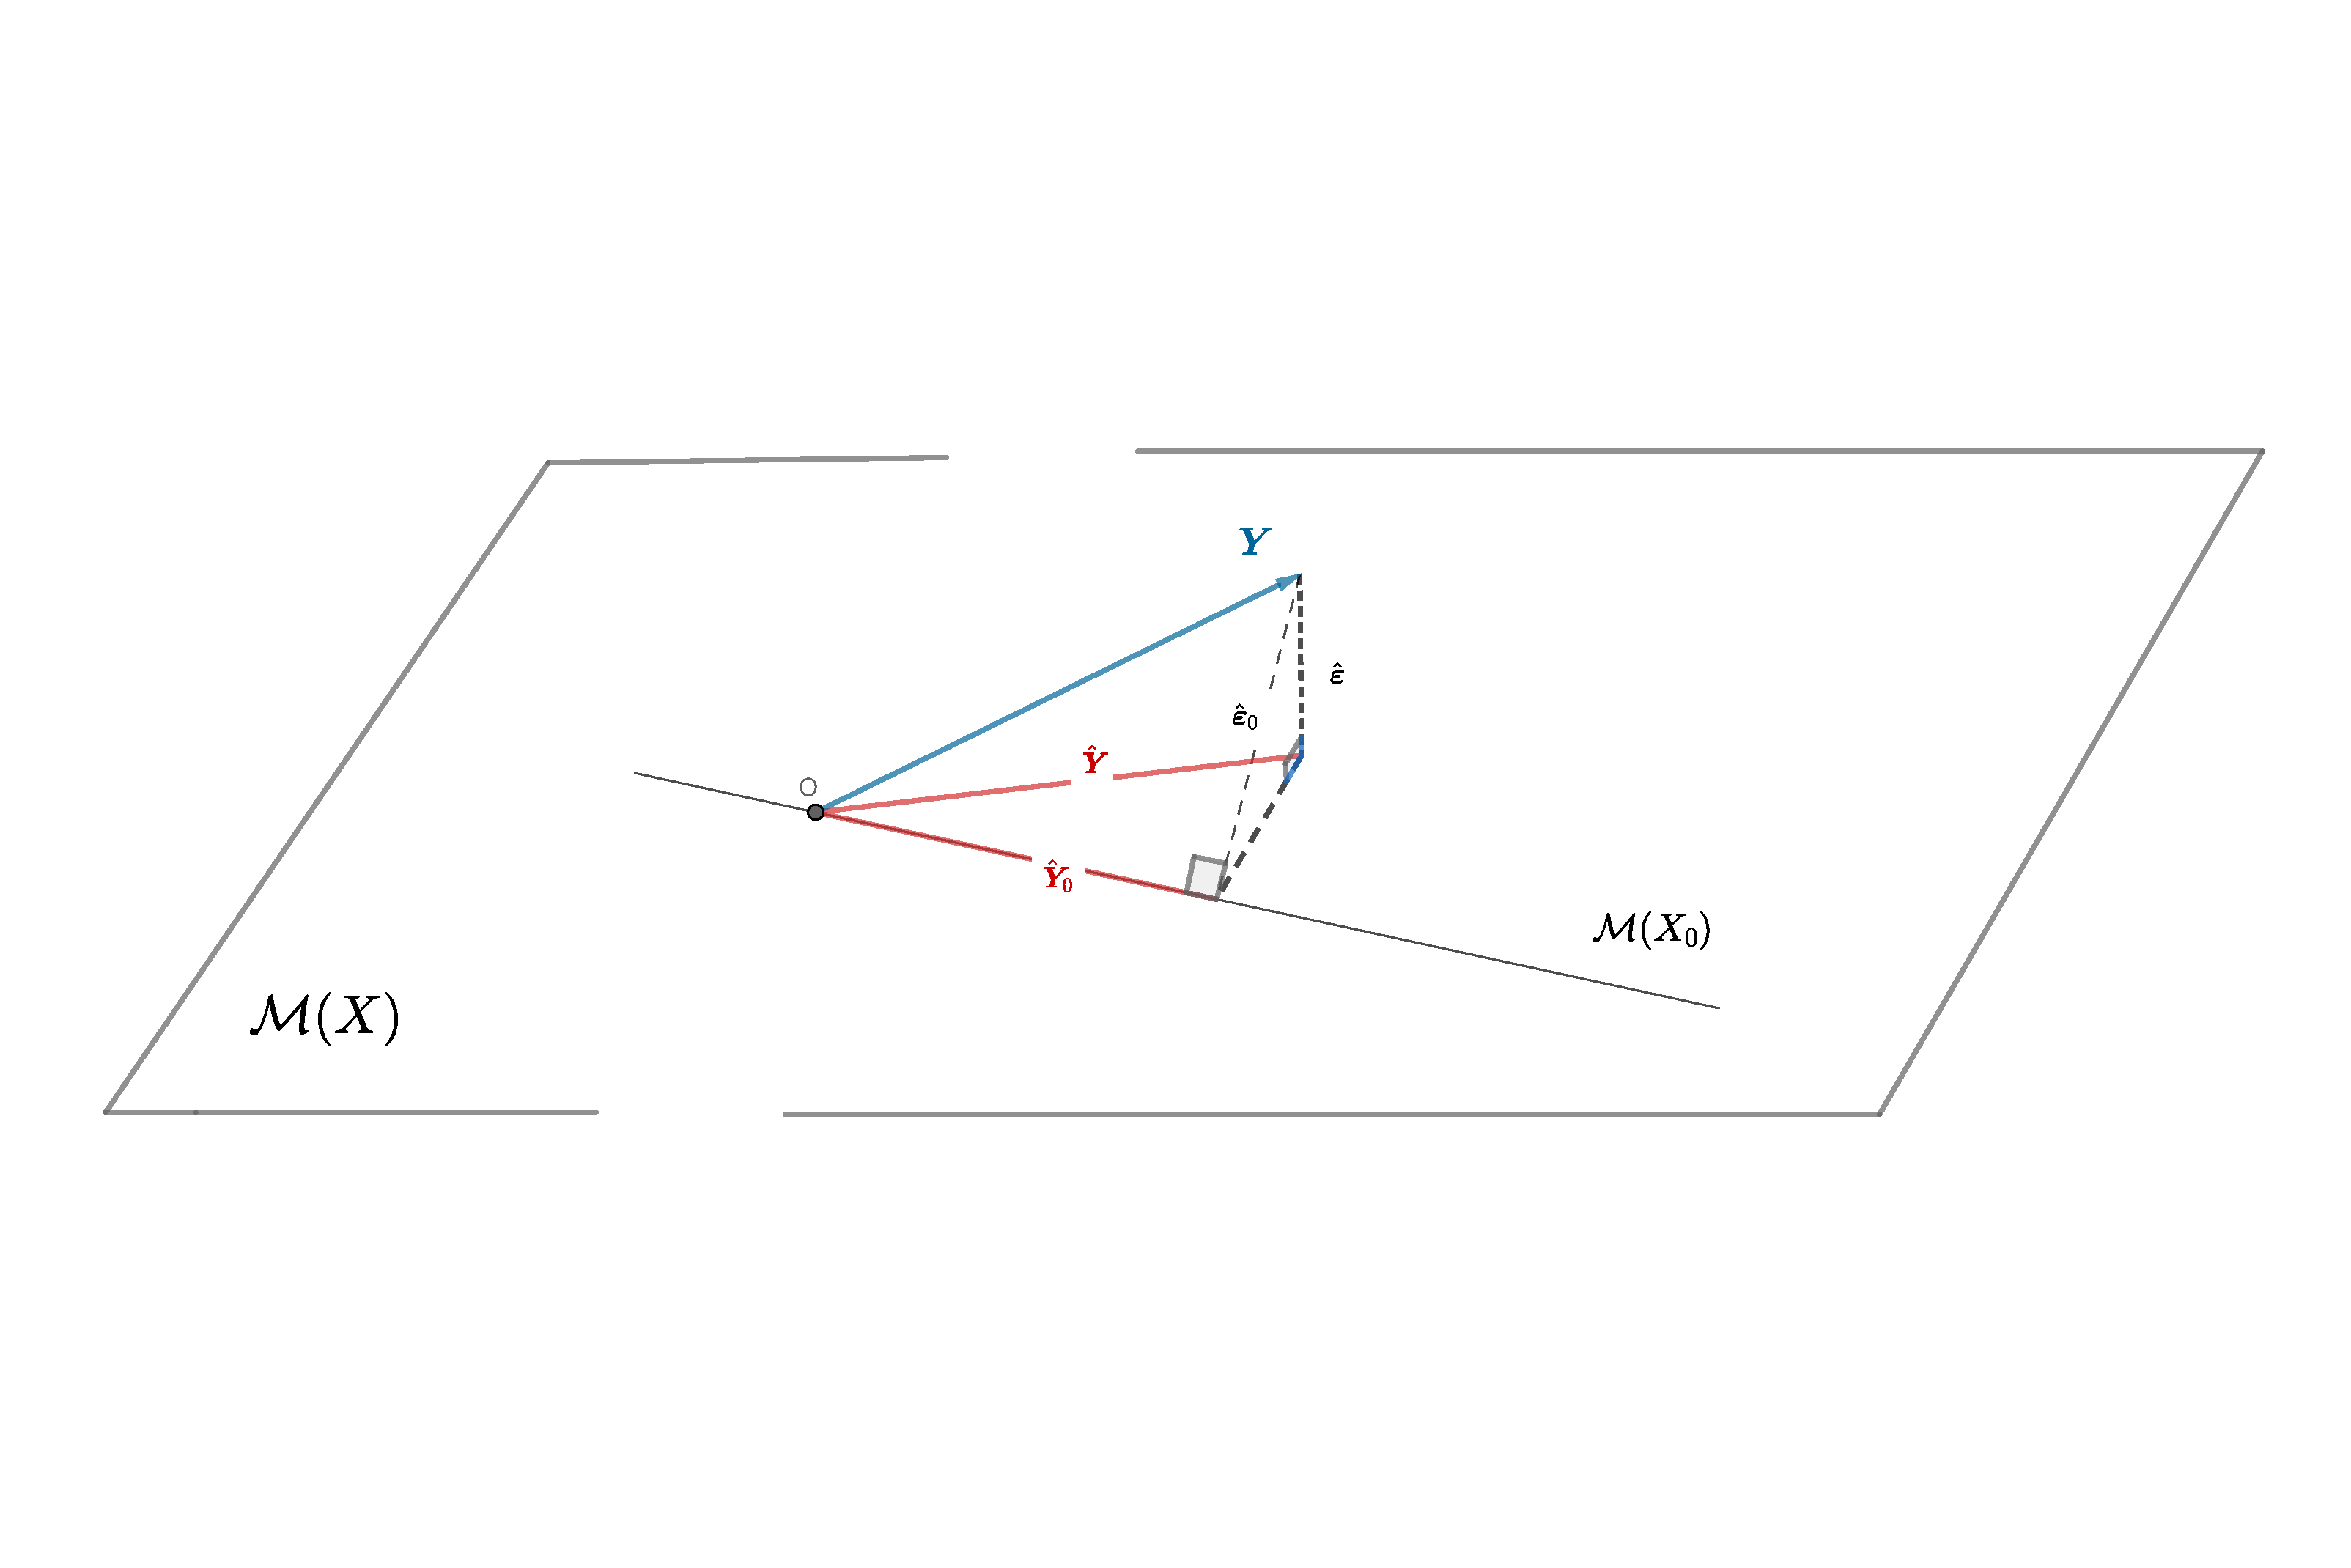
\includegraphics[width=0.7\linewidth]{images/sem2/RegMult_p3} \end{center}

Ideea procedurii de testare, și prin urmare a deciziei de a respinge sau
nu ipoteza nulă, este următoarea: dacă proiecția
\(\hat{\boldsymbol Y}_0\) a lui \(\boldsymbol Y\) pe
\(\mathcal{M}(X_0)\) este \emph{aproape} de proiecția
\(\hat{\boldsymbol Y}\) a lui \(\boldsymbol Y\) pe \(\mathcal{M}(X)\)
atunci nu respingem ipoteza nulă, în caz contrar o respingem în favoarea
alternativei \(H_1\). De fapt, dacă informația adusă de cele două modele
nu diferă foarte mult atunci este recomandat să păstrăm modelul mai
simplu (principiul parcimoniei).

Pentru a cuantifica \emph{apropierea} dintre cele două proiecții putem
considera distanța euclidiană
\(\lVert\hat{\boldsymbol Y} - \hat{\boldsymbol Y}_0\rVert^2\) dintre
acestea. Această distanță variază în funcție de datele și de unitățile
de măsură a acestora și pentru a evita această problemă de scară se
recomandă \emph{standardizarea} acestei distanțe prin împărțirea ei la
pătratul normei erorii reziduale
\(\lVert\hat{\boldsymbol \varepsilon}\rVert^2 = \lVert\boldsymbol Y - \hat{\boldsymbol Y}\rVert^2 = [n - (p+1)]\hat{\sigma}^2\).
Cum vectorii aleatori \(\hat{\boldsymbol Y} - \hat{\boldsymbol Y}_0\) și
\(\hat{\boldsymbol \varepsilon}\) nu aparțin în subspații de aceeași
dimensiune trebuie să îi împărțim și prin gradele de libertate
corespunzătoare, respectiv \(q = p+1 - p_0\) și \(n - (p+1)\). Obținem
astfel statistica de test

\[
  F = \frac{\frac{\lVert\hat{\boldsymbol Y} - \hat{\boldsymbol Y}_0\rVert^2}{p+1-p_0}}{\frac{\lVert\boldsymbol Y - \hat{\boldsymbol Y}\rVert^2}{n - (p+1)}} = \frac{n - (p+1)}{(p+1) - p_0}\frac{\lVert\hat{\boldsymbol Y} - \hat{\boldsymbol Y}_0\rVert^2}{\lVert\boldsymbol Y - \hat{\boldsymbol Y}\rVert^2}.
\]

Pentru a putea utiliza această statistică de test este necesar să
determinăm repartiția sa sub ipoteza nulă. Notând cu \(P_X\) și
respectiv \(P_{X_0}\) matricele de proiecție ortogonală pe
\(\mathcal{M}(X)\) și \(\mathcal{M}(X_0)\), știm că

\[
  \hat{\boldsymbol Y} - \hat{\boldsymbol Y}_0 = P_X\boldsymbol Y - P_{X_{0}}\boldsymbol Y
\]

și cum \(\mathcal{M}(X_0)\subset \mathcal{M}(X)\), deci
\(P_{X_0}\boldsymbol Y = P_{X_0}P_{X}\boldsymbol Y\) și

\[
  \hat{\boldsymbol Y} - \hat{\boldsymbol Y}_0 = P_{X}\boldsymbol Y -  P_{X_0}\boldsymbol Y =  (I_n - P_{X_0})P_X\boldsymbol Y = P_{X_0}^\perp P_{X}\boldsymbol Y.
\]

Astfel am găsit că
\(\hat{\boldsymbol Y} - \hat{\boldsymbol Y}_0\in\mathcal{M}(X_0)^\perp\cap \mathcal{M}(X)\)
și cum \(\boldsymbol Y - \hat{\boldsymbol Y}\in\mathcal{M}(X)^\perp\)
găsim că
\(\hat{\boldsymbol Y} - \hat{\boldsymbol Y}_0 \perp \boldsymbol Y - \hat{\boldsymbol Y}\).
Vectorii \(\hat{\boldsymbol Y} - \hat{\boldsymbol Y}_0\) și
\(\boldsymbol Y - \hat{\boldsymbol Y}\) sunt elemente din spații
ortogonale ceea ce implică
\(Cov(\hat{\boldsymbol Y} - \hat{\boldsymbol Y}_0, \boldsymbol Y - \hat{\boldsymbol Y}) - 0\)
și cum sunt și vectori gaussieni (conform ipotezei \(\mathcal{H}_2'\))
deducem că sunt și independenți ceea ce arată că numărătorul și
numitorul lui \(F\) sunt independente.

Conform Teoremei lui Cochran avem pentru numitor

\[ 
  \frac{1}{\sigma^2}\lVert\boldsymbol Y - \hat{\boldsymbol Y}\rVert^2 = \frac{1}{\sigma^2}\lVert P_{X^\perp}\boldsymbol Y\rVert^2 = \frac{1}{\sigma^2}\lVert P_{X^\perp}(\boldsymbol X\boldsymbol\beta + \boldsymbol\varepsilon)\rVert^2 = \frac{1}{\sigma^2}\lVert P_{X^\perp}\boldsymbol\varepsilon\rVert^2\sim\chi^2_{n - (p+1)}
\]

iar pentru numărător

\[
\frac{1}{\sigma^2}\lVert\hat{\boldsymbol Y} - \hat{\boldsymbol Y}_0\rVert^2 = \frac{1}{\sigma^2}\lVert P_{X_0}^\perp P_{X}\boldsymbol Y\rVert^2 = \frac{1}{\sigma^2}\lVert P_{X_0}^\perp P_{X}(\boldsymbol Y - \boldsymbol X\boldsymbol\beta)\rVert^2 \sim \chi^2_{q}
\]

Sub \(H_0\), parametrul
\(\lVert P_{X_0}^\perp P_{X}\boldsymbol X\boldsymbol\beta\rVert^2\) este
nul deoarece \(\boldsymbol X\boldsymbol\beta\in\mathcal{M}(X_0)\) ceea
ce conduce la

\[
F\overset{H_0}{\sim} F_{q, n - (p+1)}.
\]

Putem observa de asemenea că aplicând Teorema lui Pitagora

\begin{align*}
  \lVert\boldsymbol Y - \hat{\boldsymbol Y}_0\rVert^2 &= \lVert\boldsymbol Y - P_X\boldsymbol Y + P_X\boldsymbol Y - P_{X_0}\boldsymbol Y\rVert^2 = \lVert (I_n - P_X)\boldsymbol Y + P_{X_0}P_X\boldsymbol Y - P_{X_0}\boldsymbol Y\rVert^2 \\
  &= \lVert P_{X^\perp}\boldsymbol Y + (I_n - P_{X_0})P_X\boldsymbol Y \rVert^2 = \lVert P_{X^\perp}\boldsymbol Y + P_{{X_0}^\perp}P_X\boldsymbol Y \rVert^2\\
  &= \lVert P_{X^\perp}\boldsymbol Y\rVert^2 + \lVert P_{{X_0}^\perp}P_X\boldsymbol Y\rVert^2 = \lVert\boldsymbol Y - \hat{\boldsymbol Y}\rVert^2 + \lVert\hat{\boldsymbol Y} - \hat{\boldsymbol Y}_0\rVert^2
\end{align*}

altfel spus

\[
\lVert\hat{\boldsymbol Y} - \hat{\boldsymbol Y}_0\rVert^2 =  \lVert\boldsymbol Y - \hat{\boldsymbol Y}_0\rVert^2 - \lVert\boldsymbol Y - \hat{\boldsymbol Y}\rVert^2 = RSS_0 - RSS.
\]

\begin{rmdexercise}
\marginnote{\enonce{24006}{}}\vspace{-7mm}

Ne propunem să testăm ipoteza nulă \(H_0:\, \beta_j = 0\) versus ipoteza
alternativă \(H_1:\, \beta_j \neq 0\). Propuneți o procedură de testare
pentru cele două ipoteze.
\end{rmdexercise}

Această problemă este un caz particular al rezultatului obținut anterior
pentru \(q = 1\). Avem statistica de test

\[
  F = \frac{n - (p+1)}{1}\frac{\lVert\hat{\boldsymbol Y} - \hat{\boldsymbol Y}_0\rVert^2}{\lVert\boldsymbol Y - \hat{\boldsymbol Y}\rVert^2} = \frac{\lVert\hat{\boldsymbol Y} - \hat{\boldsymbol Y}_0\rVert^2}{\hat{\sigma}^2}
\]

cu ajutorul căreia putem construi regiunea critică

\[
  C = \{\omega\,|\,F(\omega)>F_{1, n - (p+1)}(1-\alpha)\}.
\]

Acest test este echivalent cu testul bazat pe statistica de test
repartizată student cu \(n - (p+1)\) grade de libertate (mai exact
\(F^2 = T_j\))

\[
  T_j = \frac{\hat{\beta}_j}{\hat{\sigma}_{\hat{\beta}_j}} = \frac{\hat{\beta}_j}{\hat{\sigma}\sqrt{\left[(\boldsymbol X^\intercal\boldsymbol X)^{-1}\right]_{j+1,j+1}}}.
\]

Regiunea critică a testului este

\[
  C = \left\{\omega\,|\,T_j(\omega)>t_{n - (p+1)}\left(1-\frac{\alpha}{2}\right)\right\}.
\]

Aceasta este forma sub care testul de semnificativitate pentru un
coeficient apare în \texttt{R}.

\begin{rmdexercise}
\marginnote{\enonce{24007}{}}\vspace{-7mm}

Propuneți o procedură de testare pentru ipotezele

\[
  H_0:\, \beta_1 = \ldots = \beta_p = 0 \quad \text{versus}\quad H_1:\,\exists j\in\{1,\ldots,p\}\, \beta_j\neq 0
\]
\end{rmdexercise}

Vrem să testăm dacă variabilele explicative au sau nu influență asupra
variabilei răspuns, cu alte cuvinte vrem să testăm dacă toți
coeficienții sunt nuli exceptînd constanta (\(\beta_0\)) - acesta este
testul care apare ca rezultat atunci când efectuăm sumarul modelului
liniar în \texttt{R} (comanda \texttt{summary(model)}). Suntem în cazul
particular în care \(\hat{\boldsymbol Y}_0 = \bar{y}\mathbf{1}\) și
obținem statistica de test a lui Fisher (\emph{testul global al lui
Fisher})

\[
  F = \frac{n - (p+1)}{p}\frac{\lVert\hat{\boldsymbol Y} - \hat{\boldsymbol Y}_0\rVert^2}{\lVert\boldsymbol Y - \hat{\boldsymbol Y}\rVert^2} \sim F_{p, n - (p+1)}
\] sau exprimată în termeni de coeficient de determinare

\[
  F = \frac{n - (p+1)}{p}\frac{R^2}{1 - R^2} \sim F_{p, n - (p+1)}.
\]

\begin{rmdexercise}
\marginnote{\enonce{24008}{}}\vspace{-7mm}

Vrem să testăm ipotezele

\[
H_0:\, \beta_{p_0+1} = \cdots = \beta_p = 0 \quad \text{versus}\quad H_1:\,\exists j\in\{p_0+1,\ldots,p\}\, \beta_j\neq 0
\]

cu ajutorul testului bazat pe raportul de verosimilități. Arătați că
acest test este echivalent cu testul \(F\) al lui Fisher.
\end{rmdexercise}

Testul bazat pe raportul de verosimilitate este

\[
  \Lambda(\mathbf{y})=\frac{\sup_{\theta\in\Theta_0}L(\theta|\mathbf{y})}{\sup_{\theta\in\Theta}L(\theta|\mathbf{y})},
\]

unde \(\Theta\) este spațiul parametrilor modelului, \(\Theta_0\) este
spațiul parametrilor corespunzător ipotezei nule iar
\(L(\theta|\mathbf{x})\) este funcția de verosimilitate.

Observăm că spațiul parametrilor modelului este

\[
\Theta = \left\{(\boldsymbol \beta, \sigma^2)|\,\boldsymbol \beta\in\mathbb{R}^{p+1}, \sigma^2\in (0,\infty)\right\},
\]

cel corespunzător ipotezei nule este

\[
\Theta_0 = \left\{(\boldsymbol \beta_0, \sigma^2)|\,\boldsymbol \beta_0\in\mathbb{R}^{p_0}, \sigma^2\in (0,\infty)\right\}
\]

iar funcția de verosimilitate este

\[
 L(\boldsymbol\beta, \sigma^2;\boldsymbol Y) = \prod_{i = 1}^{n}f_{Y}(y_i) = \left(\frac{1}{\sqrt{2\pi\sigma^2}}\right)^n e^{-\frac{1}{2\sigma^2}\sum_{i = 1}^{n}(y_i - \boldsymbol x_i^\intercal\boldsymbol\beta)^2} = \left(\frac{1}{\sqrt{2\pi\sigma^2}}\right)^n e^{-\frac{1}{2\sigma^2}\lVert\boldsymbol Y - \boldsymbol X\boldsymbol\beta\rVert^2}.
\]

Observăm că

\[
\sup_{\theta\in\Theta}L(\theta|\mathbf{y}) = \sup_{\boldsymbol\beta, \sigma^2} L(\boldsymbol\beta, \sigma^2;\boldsymbol Y) = L(\hat{\boldsymbol\beta}_{VM}, \hat{\sigma}^2_{VM};\boldsymbol Y)
\]

unde \(\hat{\boldsymbol\beta}_{VM}=\hat{\boldsymbol\beta}\) este
estimatorul obținut prin metoda celor mai mici pătrate iar
\(\hat{\sigma}^2_{VM} = \frac{\lVert\boldsymbol Y - \boldsymbol X\hat{\boldsymbol\beta}\rVert^2}{n} = \frac{RSS}{n}\).
Astfel găsim

\[
\sup_{\theta\in\Theta}L(\theta|\mathbf{y}) = \sup_{\boldsymbol\beta, \sigma^2} L(\boldsymbol\beta, \sigma^2;\boldsymbol Y) = \left(\frac{n}{2\pi\lVert\boldsymbol Y - \boldsymbol X\hat{\boldsymbol\beta}\rVert^2}\right)^{\frac{n}{2}}e^{-\frac{n}{2}} = \left(\frac{n}{2\pi RSS}\right)^{\frac{n}{2}}e^{-\frac{n}{2}}.
\]

Sub \(H_0\) avem

\[
sup_{\theta\in\Theta_0}L(\theta|\mathbf{y}) = \sup_{\boldsymbol\beta_0, \sigma^2\in\Theta_0} L(\boldsymbol\beta_0, \sigma^2;\boldsymbol Y) = L(\hat{\boldsymbol\beta}_{0}, \hat{\sigma}^2_{0};\boldsymbol Y) = \left(\frac{n}{2\pi RSS_{0}}\right)^{\frac{n}{2}}e^{-\frac{n}{2}}
\]

unde
\(RSS_0 = \lVert\boldsymbol Y - \boldsymbol X_0\hat{\boldsymbol\beta}_0\rVert^2\)
iar
\(\hat{\sigma}^2_{0} = \frac{\lVert\boldsymbol Y - \boldsymbol X_0\hat{\boldsymbol\beta}_0\rVert^2}{n} = \frac{RSS_0}{n}\).

Prin urmare raportul de verosimilitate devine

\[
\Lambda(\mathbf{y})=\frac{\sup_{\theta\in\Theta_0}L(\theta|\mathbf{y})}{\sup_{\theta\in\Theta}L(\theta|\mathbf{y})} = \frac{\left(\frac{n}{2\pi RSS_{0}}\right)^{\frac{n}{2}}e^{-\frac{n}{2}}}{\left(\frac{n}{2\pi RSS}\right)^{\frac{n}{2}}e^{-\frac{n}{2}}} = \left(\frac{RSS_0}{RSS}\right)^{-\frac{n}{2}}
\]

iar regiunea critică a testului se scrie (testul respinge ipoteza nulă
atunci când statistica \(\Lambda\) este suficient de mică)

\[
C = \left\{\boldsymbol Y\in\mathbb{R}^n\,|\, \Lambda(\boldsymbol Y)< \lambda_0 \right\}.
\] Observăm că pentru \(\lambda>0\), funcția
\(h(\lambda) = \lambda^{-\frac{2}{n}}-1\) este descrescătoare, adică
\(\lambda<\lambda_0\) implică \(h(\lambda)>h(\lambda_0)\). Avem

\[
h(\lambda)>h(\lambda_0) \iff \frac{RSS_0 - RSS}{RSS}>h(\lambda_0) \iff \frac{n - (p+1)}{(p+1) - p_0}\frac{RSS_0 - RSS}{RSS}>f_0
\]

unde \(f_0\) se determină din condiția

\[
\mathbb{P}_{H_0}\left(\frac{n - (p+1)}{(p+1) - p_0}\frac{RSS_0 - RSS}{RSS}>f_0\right) = \alpha
\]

și cum
\(\frac{n - (p+1)}{(p+1) - p_0}\frac{RSS_0 - RSS}{RSS}\sim F_{(p+1) - p_0, n - (p+1)}\)
conform exercițiului \ref{exo:24005} deducem că
\(f_0 = f_{(p+1) - p_0, n - (p+1)}(1-\alpha)\). Am găsit că regiunea
critică a testului bazat pe raportul de verosimilitate este identică cu
cea a testului \(F\) a lui Fisher (vezi exercițiul \ref{exo:24005}).

\renewcommand\refname{Referințe}
\bibliography{references/InstStatFin2018ref.bib}


\end{document}
